% Options for packages loaded elsewhere
\PassOptionsToPackage{unicode}{hyperref}
\PassOptionsToPackage{hyphens}{url}
%
\documentclass[
]{article}
\usepackage{lmodern}
\usepackage{amsmath}
\usepackage{ifxetex,ifluatex}
\ifnum 0\ifxetex 1\fi\ifluatex 1\fi=0 % if pdftex
  \usepackage[T1]{fontenc}
  \usepackage[utf8]{inputenc}
  \usepackage{textcomp} % provide euro and other symbols
  \usepackage{amssymb}
\else % if luatex or xetex
  \usepackage{unicode-math}
  \defaultfontfeatures{Scale=MatchLowercase}
  \defaultfontfeatures[\rmfamily]{Ligatures=TeX,Scale=1}
\fi
% Use upquote if available, for straight quotes in verbatim environments
\IfFileExists{upquote.sty}{\usepackage{upquote}}{}
\IfFileExists{microtype.sty}{% use microtype if available
  \usepackage[]{microtype}
  \UseMicrotypeSet[protrusion]{basicmath} % disable protrusion for tt fonts
}{}
\makeatletter
\@ifundefined{KOMAClassName}{% if non-KOMA class
  \IfFileExists{parskip.sty}{%
    \usepackage{parskip}
  }{% else
    \setlength{\parindent}{0pt}
    \setlength{\parskip}{6pt plus 2pt minus 1pt}}
}{% if KOMA class
  \KOMAoptions{parskip=half}}
\makeatother
\usepackage{xcolor}
\IfFileExists{xurl.sty}{\usepackage{xurl}}{} % add URL line breaks if available
\IfFileExists{bookmark.sty}{\usepackage{bookmark}}{\usepackage{hyperref}}
\hypersetup{
  pdftitle={Cars Analysis and Modeling},
  pdfauthor={Group 1: Emma Doyle, Reid Hoffmeier, Matthew Lane, Mikhail Mikhaylov, Brandon Strong},
  hidelinks,
  pdfcreator={LaTeX via pandoc}}
\urlstyle{same} % disable monospaced font for URLs
\usepackage[margin=1in]{geometry}
\usepackage{color}
\usepackage{fancyvrb}
\newcommand{\VerbBar}{|}
\newcommand{\VERB}{\Verb[commandchars=\\\{\}]}
\DefineVerbatimEnvironment{Highlighting}{Verbatim}{commandchars=\\\{\}}
% Add ',fontsize=\small' for more characters per line
\usepackage{framed}
\definecolor{shadecolor}{RGB}{248,248,248}
\newenvironment{Shaded}{\begin{snugshade}}{\end{snugshade}}
\newcommand{\AlertTok}[1]{\textcolor[rgb]{0.94,0.16,0.16}{#1}}
\newcommand{\AnnotationTok}[1]{\textcolor[rgb]{0.56,0.35,0.01}{\textbf{\textit{#1}}}}
\newcommand{\AttributeTok}[1]{\textcolor[rgb]{0.77,0.63,0.00}{#1}}
\newcommand{\BaseNTok}[1]{\textcolor[rgb]{0.00,0.00,0.81}{#1}}
\newcommand{\BuiltInTok}[1]{#1}
\newcommand{\CharTok}[1]{\textcolor[rgb]{0.31,0.60,0.02}{#1}}
\newcommand{\CommentTok}[1]{\textcolor[rgb]{0.56,0.35,0.01}{\textit{#1}}}
\newcommand{\CommentVarTok}[1]{\textcolor[rgb]{0.56,0.35,0.01}{\textbf{\textit{#1}}}}
\newcommand{\ConstantTok}[1]{\textcolor[rgb]{0.00,0.00,0.00}{#1}}
\newcommand{\ControlFlowTok}[1]{\textcolor[rgb]{0.13,0.29,0.53}{\textbf{#1}}}
\newcommand{\DataTypeTok}[1]{\textcolor[rgb]{0.13,0.29,0.53}{#1}}
\newcommand{\DecValTok}[1]{\textcolor[rgb]{0.00,0.00,0.81}{#1}}
\newcommand{\DocumentationTok}[1]{\textcolor[rgb]{0.56,0.35,0.01}{\textbf{\textit{#1}}}}
\newcommand{\ErrorTok}[1]{\textcolor[rgb]{0.64,0.00,0.00}{\textbf{#1}}}
\newcommand{\ExtensionTok}[1]{#1}
\newcommand{\FloatTok}[1]{\textcolor[rgb]{0.00,0.00,0.81}{#1}}
\newcommand{\FunctionTok}[1]{\textcolor[rgb]{0.00,0.00,0.00}{#1}}
\newcommand{\ImportTok}[1]{#1}
\newcommand{\InformationTok}[1]{\textcolor[rgb]{0.56,0.35,0.01}{\textbf{\textit{#1}}}}
\newcommand{\KeywordTok}[1]{\textcolor[rgb]{0.13,0.29,0.53}{\textbf{#1}}}
\newcommand{\NormalTok}[1]{#1}
\newcommand{\OperatorTok}[1]{\textcolor[rgb]{0.81,0.36,0.00}{\textbf{#1}}}
\newcommand{\OtherTok}[1]{\textcolor[rgb]{0.56,0.35,0.01}{#1}}
\newcommand{\PreprocessorTok}[1]{\textcolor[rgb]{0.56,0.35,0.01}{\textit{#1}}}
\newcommand{\RegionMarkerTok}[1]{#1}
\newcommand{\SpecialCharTok}[1]{\textcolor[rgb]{0.00,0.00,0.00}{#1}}
\newcommand{\SpecialStringTok}[1]{\textcolor[rgb]{0.31,0.60,0.02}{#1}}
\newcommand{\StringTok}[1]{\textcolor[rgb]{0.31,0.60,0.02}{#1}}
\newcommand{\VariableTok}[1]{\textcolor[rgb]{0.00,0.00,0.00}{#1}}
\newcommand{\VerbatimStringTok}[1]{\textcolor[rgb]{0.31,0.60,0.02}{#1}}
\newcommand{\WarningTok}[1]{\textcolor[rgb]{0.56,0.35,0.01}{\textbf{\textit{#1}}}}
\usepackage{longtable,booktabs}
\usepackage{calc} % for calculating minipage widths
% Correct order of tables after \paragraph or \subparagraph
\usepackage{etoolbox}
\makeatletter
\patchcmd\longtable{\par}{\if@noskipsec\mbox{}\fi\par}{}{}
\makeatother
% Allow footnotes in longtable head/foot
\IfFileExists{footnotehyper.sty}{\usepackage{footnotehyper}}{\usepackage{footnote}}
\makesavenoteenv{longtable}
\usepackage{graphicx}
\makeatletter
\def\maxwidth{\ifdim\Gin@nat@width>\linewidth\linewidth\else\Gin@nat@width\fi}
\def\maxheight{\ifdim\Gin@nat@height>\textheight\textheight\else\Gin@nat@height\fi}
\makeatother
% Scale images if necessary, so that they will not overflow the page
% margins by default, and it is still possible to overwrite the defaults
% using explicit options in \includegraphics[width, height, ...]{}
\setkeys{Gin}{width=\maxwidth,height=\maxheight,keepaspectratio}
% Set default figure placement to htbp
\makeatletter
\def\fps@figure{htbp}
\makeatother
\setlength{\emergencystretch}{3em} % prevent overfull lines
\providecommand{\tightlist}{%
  \setlength{\itemsep}{0pt}\setlength{\parskip}{0pt}}
\setcounter{secnumdepth}{-\maxdimen} % remove section numbering
\ifluatex
  \usepackage{selnolig}  % disable illegal ligatures
\fi

\title{Cars Analysis and Modeling}
\author{Group 1: Emma Doyle, Reid Hoffmeier, Matthew Lane, Mikhail
Mikhaylov, Brandon Strong}
\date{5/15/2021}

\begin{document}
\maketitle

\hypertarget{abstract}{%
\section{Abstract}\label{abstract}}

Vehicles are essential to transportation as a society, and one of the
main methods of obtaining a vehicle is through the purchase of a
previously owned vehicle. Belarus, as with many countries, has an
extensive used vehicle market that will be extensively studied. A
popular used cars catalog from the country of Belarus will be cleaned
and analyzed to answer several questions as well as accomplish our main
two goals. Multiple Linear Regression, SVR, Decision Tree Regression,
Random Forest Regression, and KNN will all be used to predict the market
price of a used car in Belarus given the attributes found in the
dataset. Also, a Decision Tree and a Logistic Regression Model will be
used to create an exploratory and predictive model for the exchange
preferences of a vehicle owner in Belarus. The accuracy of these models
will be analyzed, and performance tested for real-world application with
the help of a training and testing dataset.

\textbf{OUR FINDINGS:} We found that the Random forest tree had the best
R-Squared value, lowest error rate, and lowest RMSE which tells us that
this model technique is the best of all the models tested for making
predictions from our dataset. The two worst prediction models were the
Multiple Linear Regression, and SVR Radial. Below is a chart of all our
results from each of our models. We note that a lower error rate is
better, and the higher the R-Squared value the better the correlation
the model has with the data.

\begin{longtable}[]{@{}lccr@{}}
\toprule
Machine-Learning Methods & RMSE & Error Rate & R-Square\tabularnewline
\midrule
\endhead
Multiple Linear Regression & \textbf{4470.274} & \textbf{67.57975} &
\textbf{0.5190641}\tabularnewline
SVR Linear & \textbf{3257.887} & \textbf{48.86921} &
\textbf{0.7772176}\tabularnewline
SVR Radial & \textbf{4752.231} & \textbf{71.28478} &
\textbf{0.5937837}\tabularnewline
Decision Tree Regression & \textbf{3245.413} & \textbf{48.68209} &
\textbf{0.7529956}\tabularnewline
Random Forest Tree Regression & \textbf{1879.884} & \textbf{28.19878} &
\textbf{0.9184761}\tabularnewline
KNN(K Nearest Neighbor) & \textbf{3693.939} & \textbf{55.41011} &
\textbf{0.680185}\tabularnewline
\bottomrule
\end{longtable}

Lastly, we employed used two different models to test whether the
vehicle owner was willing to exchange his vehicle. The two models that
were used were the decision tree and logistic classification. Both trees
were very similar; however, the decision tree was determined to perform
slightly better as an exploratory and predictive model. The results of
the models are as follows:

\begin{longtable}[]{@{}lllllll@{}}
\toprule
\begin{minipage}[b]{(\columnwidth - 6\tabcolsep) * \real{0.35}}\raggedright
Models\strut
\end{minipage} &
\begin{minipage}[b]{(\columnwidth - 6\tabcolsep) * \real{0.08}}\raggedright
Accuracy\strut
\end{minipage} &
\begin{minipage}[b]{(\columnwidth - 6\tabcolsep) * \real{0.08}}\raggedright
Error\strut
\end{minipage} &
\begin{minipage}[b]{(\columnwidth - 6\tabcolsep) * \real{0.10}}\raggedright
Sensitivity\strut
\end{minipage} &
\begin{minipage}[b]{(\columnwidth - 6\tabcolsep) * \real{0.10}}\raggedright
Specificity\strut
\end{minipage} &
\begin{minipage}[b]{(\columnwidth - 6\tabcolsep) * \real{0.20}}\raggedright
Positive Prediction Value\strut
\end{minipage} &
\begin{minipage}[b]{(\columnwidth - 6\tabcolsep) * \real{0.08}}\raggedright
AUC\strut
\end{minipage}\tabularnewline
\midrule
\endhead
\begin{minipage}[t]{(\columnwidth - 6\tabcolsep) * \real{0.35}}\raggedright
Decision Tree Classification: Exploratory Model\strut
\end{minipage} &
\begin{minipage}[t]{(\columnwidth - 6\tabcolsep) * \real{0.08}}\raggedright
0.6939802\strut
\end{minipage} &
\begin{minipage}[t]{(\columnwidth - 6\tabcolsep) * \real{0.08}}\raggedright
0.3060198\strut
\end{minipage} &
\begin{minipage}[t]{(\columnwidth - 6\tabcolsep) * \real{0.10}}\raggedright
0.6349\strut
\end{minipage} &
\begin{minipage}[t]{(\columnwidth - 6\tabcolsep) * \real{0.10}}\raggedright
0.7064\strut
\end{minipage} &
\begin{minipage}[t]{(\columnwidth - 6\tabcolsep) * \real{0.20}}\raggedright
0.3116\strut
\end{minipage} &
\begin{minipage}[t]{(\columnwidth - 6\tabcolsep) * \real{0.08}}\raggedright
0.6571428\strut
\end{minipage}\tabularnewline
\begin{minipage}[t]{(\columnwidth - 6\tabcolsep) * \real{0.35}}\raggedright
Logistic Classification: Exploratory Model\strut
\end{minipage} &
\begin{minipage}[t]{(\columnwidth - 6\tabcolsep) * \real{0.08}}\raggedright
0.6624371\strut
\end{minipage} &
\begin{minipage}[t]{(\columnwidth - 6\tabcolsep) * \real{0.08}}\raggedright
0.3375629\strut
\end{minipage} &
\begin{minipage}[t]{(\columnwidth - 6\tabcolsep) * \real{0.10}}\raggedright
0.58457\strut
\end{minipage} &
\begin{minipage}[t]{(\columnwidth - 6\tabcolsep) * \real{0.10}}\raggedright
0.67010\strut
\end{minipage} &
\begin{minipage}[t]{(\columnwidth - 6\tabcolsep) * \real{0.20}}\raggedright
0.14850\strut
\end{minipage} &
\begin{minipage}[t]{(\columnwidth - 6\tabcolsep) * \real{0.08}}\raggedright
0.6505955\strut
\end{minipage}\tabularnewline
\begin{minipage}[t]{(\columnwidth - 6\tabcolsep) * \real{0.35}}\raggedright
Decision Tree Classification: Prediction Model\strut
\end{minipage} &
\begin{minipage}[t]{(\columnwidth - 6\tabcolsep) * \real{0.08}}\raggedright
0.6871661\strut
\end{minipage} &
\begin{minipage}[t]{(\columnwidth - 6\tabcolsep) * \real{0.08}}\raggedright
0.3128339\strut
\end{minipage} &
\begin{minipage}[t]{(\columnwidth - 6\tabcolsep) * \real{0.10}}\raggedright
0.6062\strut
\end{minipage} &
\begin{minipage}[t]{(\columnwidth - 6\tabcolsep) * \real{0.10}}\raggedright
0.7039\strut
\end{minipage} &
\begin{minipage}[t]{(\columnwidth - 6\tabcolsep) * \real{0.20}}\raggedright
0.2980\strut
\end{minipage} &
\begin{minipage}[t]{(\columnwidth - 6\tabcolsep) * \real{0.08}}\raggedright
0.6525616\strut
\end{minipage}\tabularnewline
\begin{minipage}[t]{(\columnwidth - 6\tabcolsep) * \real{0.35}}\raggedright
Logistic Classification: Prediction Model\strut
\end{minipage} &
\begin{minipage}[t]{(\columnwidth - 6\tabcolsep) * \real{0.08}}\raggedright
0.6650163\strut
\end{minipage} &
\begin{minipage}[t]{(\columnwidth - 6\tabcolsep) * \real{0.08}}\raggedright
0.3349837\strut
\end{minipage} &
\begin{minipage}[t]{(\columnwidth - 6\tabcolsep) * \real{0.10}}\raggedright
0.58041\strut
\end{minipage} &
\begin{minipage}[t]{(\columnwidth - 6\tabcolsep) * \real{0.10}}\raggedright
0.67329\strut
\end{minipage} &
\begin{minipage}[t]{(\columnwidth - 6\tabcolsep) * \real{0.20}}\raggedright
0.14808\strut
\end{minipage} &
\begin{minipage}[t]{(\columnwidth - 6\tabcolsep) * \real{0.08}}\raggedright
0.6480223\strut
\end{minipage}\tabularnewline
\bottomrule
\end{longtable}

The AUC, accuracy, sensitivity, and specificity are higher in the
decision tree. All these values allow us to conclude that the Decision
Tree produces a better predictive model. Nevertheless, both models
produce good predictive and exploratory of whether a vehicle owner is
willing to exchange a vehicle.

\hypertarget{introduction}{%
\section{Introduction}\label{introduction}}

\hypertarget{focus-problems}{%
\subsection{Focus Problems}\label{focus-problems}}

There are several objectives that will be the focal point of the
research done on the used cars dataset. The main scope of this project
is to create an effective predictive model for the price of a used in
Vehicle in Belarus. An exploratory and predictive model will be created
for the likelihood of a vehicle owner being willing to exchange their
vehicle. Several questions will be answered in the process of creating
the following models and to gain a further understanding of the overall
dataset.

\hypertarget{problem-motivations}{%
\subsection{Problem Motivations}\label{problem-motivations}}

The popularity of the used vehicle market and personal experience in
buying a vehicle led to initial intrigue in the used dataset.
Furthermore, having a project member who was born in Eastern Europe led
to added interest in how the vehicle market differs from the used car
market in America. Interest in what factors contributed the most to a
vehicles price, and the desire to successfully predict a vehicles price
given those factors led to the desire to produce predictive models for
price. Also, personal experience with vehicle owners offering vehicle
exchanges motivated the desire to create an exploratory and predictive
model for the willingness of an owner to offer an exchange.

\hypertarget{problem-solving-methodology}{%
\subsection{Problem Solving
Methodology}\label{problem-solving-methodology}}

To solve our questions and answer our goal we are going to use R to make
graphs to answer our questions. We will make sure to use different
statistical analyses to make sure our graphs are confirmed to be
accurate. The use of the Chi-Square Test, Anova Test, as well as the
Correlation Test will be extensive to answer our questions. Furthermore,
the dataset will be split into a training and testing set to verify the
accuracies of the models that will be produced. Several models will be
tested to achieve the most accurate result and these accuracies will be
verified using RMSE, R-Squared, and error rate for regression models as
well as accuracy, sensitivity, specificity, and AUC for the
classification models.

\hypertarget{initial-questions}{%
\section{Initial Questions}\label{initial-questions}}

The main goal is to create a predictive model based on insights gained
from analyzing the impact of variables on the selling price of a
vehicle. The goal was chosen for its applicability and general interest
in which attributes impact price of a used car. Secondly, exploratory,
and predictive models to gauge whether a vehicle would be exchangeable
or not will be created using a Decision Tree and Logistic
Classification. Both these models will be analyzed for accuracy,
sensitivity, and specificity. In addition, there will be several
questions that will be answered concerning the dataset. These questions
aid in solving the main goal and are important insights to be gleaned
from the dataset. The questions that will be answered about the dataset
are as follows:

\begin{itemize}
\tightlist
\item
  What impact does a region have on price?
\item
  What is the distribution of manufacturers and whether manufacturers
  have a significant impact on the asking price of a vehicle?
\item
  What is the relationship between odometer and price?
\item
  Does the number of photos a vehicle has impact the selling price?
\item
  Does the number of times a vehicle has been upped in the catalog to
  raise its position impact the selling price?
\item
  Relationship between Engine Type and Body Type? What is the impact of
  Engine Type and Body Type on the selling price?
\item
  What is the most popular model and whether we can conclude that the
  popularity of a model has a direct impact on the price of a vehicle?
\item
  What is the average age of each vehicle manufacturer and whether the
  manufacturer changes how the production year impacts the selling
  price?
\end{itemize}

\hypertarget{dataset}{%
\section{Dataset}\label{dataset}}

\hypertarget{dataset-source}{%
\subsection{Dataset Source}\label{dataset-source}}

Kaggle dataset:
\href{https://www.kaggle.com/lepchenkov/usedcarscatalog}{Used Cars
Catalog}.

The dataset that was chosen was obtained from Kaggle and was scraped by
an individual named Kirill Lepchenkov with the help of an associate
named Vasily Kachalko who aided in parsing the data. This dataset will
be utilized to understand the effect certain characteristics have on the
price point at which cars in Belarus are sold at. Analyzing cars that
are for sale is beneficial in gaining an understanding on what
contributes to how a used car would be priced and would allow for
predicting the market price of a used car in Belarus.

\hypertarget{dataset-description}{%
\subsection{Dataset Description}\label{dataset-description}}

This dataset has 30 attributes with 38,531 samples. Of these attributes
there is a mixture of Categorical (Nominal) as well as Numerical
(Interval, Ratio) data. The attributes included in the dataset are
Manufacturer Name, Model Name, Transmission Type, Color, Odometer Value,
Year Produced, Engine Fuel, Engine Has Gas(Boolean), Engine Type, Engine
Capacity, Body Type, Has Warranty(Boolean), (State) Condition of the
Vehicle, Drivetrain Type, Price in USD, Exchangeability (Boolean),
Location Region, Number of Photos, Number of Up Counts, Features
\{0,1,2,3,4,5,6,7,8,9\}, and Duration Listed.

\hypertarget{data-cleaning}{%
\subsection{Data Cleaning}\label{data-cleaning}}

To clean the dataset, it was vital to open the csv file and investigate
the types of attributes and samples that were given. To get a quick
glance of the data we first open the csv file as follows:

\begin{Shaded}
\begin{Highlighting}[]
\NormalTok{cars }\OtherTok{\textless{}{-}} \FunctionTok{read\_csv}\NormalTok{(}\StringTok{"cars.csv"}\NormalTok{)}
\end{Highlighting}
\end{Shaded}

\begin{verbatim}
## 
## -- Column specification --------------------------------------------------------
## cols(
##   .default = col_logical(),
##   manufacturer_name = col_character(),
##   model_name = col_character(),
##   transmission = col_character(),
##   color = col_character(),
##   odometer_value = col_double(),
##   year_produced = col_double(),
##   engine_fuel = col_character(),
##   engine_type = col_character(),
##   engine_capacity = col_double(),
##   body_type = col_character(),
##   state = col_character(),
##   drivetrain = col_character(),
##   price_usd = col_double(),
##   location_region = col_character(),
##   number_of_photos = col_double(),
##   up_counter = col_double(),
##   duration_listed = col_double()
## )
## i Use `spec()` for the full column specifications.
\end{verbatim}

\begin{Shaded}
\begin{Highlighting}[]
\FunctionTok{head}\NormalTok{(cars, }\DecValTok{20}\NormalTok{)}
\end{Highlighting}
\end{Shaded}

\begin{verbatim}
## # A tibble: 20 x 30
##    manufacturer_name model_name transmission color  odometer_value year_produced
##    <chr>             <chr>      <chr>        <chr>           <dbl>         <dbl>
##  1 Subaru            Outback    automatic    silver         190000          2010
##  2 Subaru            Outback    automatic    blue           290000          2002
##  3 Subaru            Forester   automatic    red            402000          2001
##  4 Subaru            Impreza    mechanical   blue            10000          1999
##  5 Subaru            Legacy     automatic    black          280000          2001
##  6 Subaru            Outback    automatic    silver         132449          2011
##  7 Subaru            Forester   automatic    black          318280          1998
##  8 Subaru            Legacy     automatic    silver         350000          2004
##  9 Subaru            Outback    automatic    grey           179000          2010
## 10 Subaru            Forester   automatic    silver         571317          1999
## 11 Subaru            Forester   mechanical   other          280000          2003
## 12 Subaru            Tribeca    automatic    grey           256000          2008
## 13 Subaru            Forester   mechanical   other          321000          2002
## 14 Subaru            Justy      mechanical   red             49999          2001
## 15 Subaru            Outback    automatic    brown          154685          2011
## 16 Subaru            Outback    automatic    black          163219          2004
## 17 Subaru            Outback    automatic    other          318650          2005
## 18 Subaru            Impreza    mechanical   blue           191000          2005
## 19 Subaru            Forester   automatic    silver         179000          2014
## 20 Subaru            Forester   automatic    black          159000          2013
## # ... with 24 more variables: engine_fuel <chr>, engine_has_gas <lgl>,
## #   engine_type <chr>, engine_capacity <dbl>, body_type <chr>,
## #   has_warranty <lgl>, state <chr>, drivetrain <chr>, price_usd <dbl>,
## #   is_exchangeable <lgl>, location_region <chr>, number_of_photos <dbl>,
## #   up_counter <dbl>, feature_0 <lgl>, feature_1 <lgl>, feature_2 <lgl>,
## #   feature_3 <lgl>, feature_4 <lgl>, feature_5 <lgl>, feature_6 <lgl>,
## #   feature_7 <lgl>, feature_8 <lgl>, feature_9 <lgl>, duration_listed <dbl>
\end{verbatim}

Afterwards, it was crucial to obtain a quick summary of our dataset to
assess the steps needed to clean the dataset. This was done with the
following line of code:

\begin{Shaded}
\begin{Highlighting}[]
\FunctionTok{summary}\NormalTok{(cars)}
\end{Highlighting}
\end{Shaded}

\begin{verbatim}
##  manufacturer_name   model_name        transmission          color          
##  Length:38531       Length:38531       Length:38531       Length:38531      
##  Class :character   Class :character   Class :character   Class :character  
##  Mode  :character   Mode  :character   Mode  :character   Mode  :character  
##                                                                             
##                                                                             
##                                                                             
##                                                                             
##  odometer_value    year_produced  engine_fuel        engine_has_gas 
##  Min.   :      0   Min.   :1942   Length:38531       Mode :logical  
##  1st Qu.: 158000   1st Qu.:1998   Class :character   FALSE:37184    
##  Median : 250000   Median :2003   Mode  :character   TRUE :1347     
##  Mean   : 248865   Mean   :2003                                     
##  3rd Qu.: 325000   3rd Qu.:2009                                     
##  Max.   :1000000   Max.   :2019                                     
##                                                                     
##  engine_type        engine_capacity  body_type         has_warranty   
##  Length:38531       Min.   :0.200   Length:38531       Mode :logical  
##  Class :character   1st Qu.:1.600   Class :character   FALSE:38082    
##  Mode  :character   Median :2.000   Mode  :character   TRUE :449      
##                     Mean   :2.055                                     
##                     3rd Qu.:2.300                                     
##                     Max.   :8.000                                     
##                     NA's   :10                                        
##     state            drivetrain          price_usd     is_exchangeable
##  Length:38531       Length:38531       Min.   :    1   Mode :logical  
##  Class :character   Class :character   1st Qu.: 2100   FALSE:24945    
##  Mode  :character   Mode  :character   Median : 4800   TRUE :13586    
##                                        Mean   : 6640                  
##                                        3rd Qu.: 8990                  
##                                        Max.   :50000                  
##                                                                       
##  location_region    number_of_photos   up_counter      feature_0      
##  Length:38531       Min.   : 1.000   Min.   :   1.00   Mode :logical  
##  Class :character   1st Qu.: 5.000   1st Qu.:   2.00   FALSE:29725    
##  Mode  :character   Median : 8.000   Median :   5.00   TRUE :8806     
##                     Mean   : 9.649   Mean   :  16.31                  
##                     3rd Qu.:12.000   3rd Qu.:  16.00                  
##                     Max.   :86.000   Max.   :1861.00                  
##                                                                       
##  feature_1       feature_2       feature_3       feature_4      
##  Mode :logical   Mode :logical   Mode :logical   Mode :logical  
##  FALSE:15135     FALSE:29907     FALSE:27904     FALSE:29227    
##  TRUE :23396     TRUE :8624      TRUE :10627     TRUE :9304     
##                                                                 
##                                                                 
##                                                                 
##                                                                 
##  feature_5       feature_6       feature_7       feature_8      
##  Mode :logical   Mode :logical   Mode :logical   Mode :logical  
##  FALSE:24811     FALSE:31943     FALSE:28369     FALSE:22528    
##  TRUE :13720     TRUE :6588      TRUE :10162     TRUE :16003    
##                                                                 
##                                                                 
##                                                                 
##                                                                 
##  feature_9       duration_listed  
##  Mode :logical   Min.   :   0.00  
##  FALSE:16206     1st Qu.:  23.00  
##  TRUE :22325     Median :  59.00  
##                  Mean   :  80.58  
##                  3rd Qu.:  91.00  
##                  Max.   :2232.00  
## 
\end{verbatim}

From the summary we clearly see that engine\_has\_gas, has\_warranty,
and state have very little variability and for that reason they will be
removed from the dataset. Furthermore, upon researching the features
attribute it was uncovered that the data had severe inconsistencies
(according to the creator) and for that reason they will be removed. To
accomplish this, we run the select command to remove these attributes.

\begin{Shaded}
\begin{Highlighting}[]
\NormalTok{cars\_edited }\OtherTok{\textless{}{-}}\NormalTok{ dplyr}\SpecialCharTok{::}\FunctionTok{select}\NormalTok{(cars, }\SpecialCharTok{{-}}\DecValTok{8} \SpecialCharTok{\&} \SpecialCharTok{{-}}\NormalTok{(}\DecValTok{12}\SpecialCharTok{:}\DecValTok{13}\NormalTok{) }\SpecialCharTok{\&} \SpecialCharTok{{-}}\NormalTok{(}\DecValTok{20}\SpecialCharTok{:}\DecValTok{29}\NormalTok{))}
\FunctionTok{head}\NormalTok{(cars\_edited, }\DecValTok{20}\NormalTok{)}
\end{Highlighting}
\end{Shaded}

\begin{verbatim}
## # A tibble: 20 x 17
##    manufacturer_name model_name transmission color  odometer_value year_produced
##    <chr>             <chr>      <chr>        <chr>           <dbl>         <dbl>
##  1 Subaru            Outback    automatic    silver         190000          2010
##  2 Subaru            Outback    automatic    blue           290000          2002
##  3 Subaru            Forester   automatic    red            402000          2001
##  4 Subaru            Impreza    mechanical   blue            10000          1999
##  5 Subaru            Legacy     automatic    black          280000          2001
##  6 Subaru            Outback    automatic    silver         132449          2011
##  7 Subaru            Forester   automatic    black          318280          1998
##  8 Subaru            Legacy     automatic    silver         350000          2004
##  9 Subaru            Outback    automatic    grey           179000          2010
## 10 Subaru            Forester   automatic    silver         571317          1999
## 11 Subaru            Forester   mechanical   other          280000          2003
## 12 Subaru            Tribeca    automatic    grey           256000          2008
## 13 Subaru            Forester   mechanical   other          321000          2002
## 14 Subaru            Justy      mechanical   red             49999          2001
## 15 Subaru            Outback    automatic    brown          154685          2011
## 16 Subaru            Outback    automatic    black          163219          2004
## 17 Subaru            Outback    automatic    other          318650          2005
## 18 Subaru            Impreza    mechanical   blue           191000          2005
## 19 Subaru            Forester   automatic    silver         179000          2014
## 20 Subaru            Forester   automatic    black          159000          2013
## # ... with 11 more variables: engine_fuel <chr>, engine_type <chr>,
## #   engine_capacity <dbl>, body_type <chr>, drivetrain <chr>, price_usd <dbl>,
## #   is_exchangeable <lgl>, location_region <chr>, number_of_photos <dbl>,
## #   up_counter <dbl>, duration_listed <dbl>
\end{verbatim}

Now, to proceed with cleaning and analyzation we need a more robust
knowledge of our dataset. For this reason, it is vital to understand the
type of data for each attribute. Therefore, we create a table to
organize all our attributes.

\begin{longtable}[]{@{}lccr@{}}
\toprule
\begin{minipage}[b]{(\columnwidth - 3\tabcolsep) * \real{0.06}}\raggedright
Column\strut
\end{minipage} &
\begin{minipage}[b]{(\columnwidth - 3\tabcolsep) * \real{0.13}}\centering
Details\strut
\end{minipage} &
\begin{minipage}[b]{(\columnwidth - 3\tabcolsep) * \real{0.73}}\centering
Value/(Units)\strut
\end{minipage} &
\begin{minipage}[b]{(\columnwidth - 3\tabcolsep) * \real{0.08}}\raggedleft
Data Type\strut
\end{minipage}\tabularnewline
\midrule
\endhead
\begin{minipage}[t]{(\columnwidth - 3\tabcolsep) * \real{0.06}}\raggedright
A\strut
\end{minipage} &
\begin{minipage}[t]{(\columnwidth - 3\tabcolsep) * \real{0.13}}\centering
Manufacturer Name\strut
\end{minipage} &
\begin{minipage}[t]{(\columnwidth - 3\tabcolsep) * \real{0.73}}\centering
Name of vehicle manufacturer\strut
\end{minipage} &
\begin{minipage}[t]{(\columnwidth - 3\tabcolsep) * \real{0.08}}\raggedleft
Nominal\strut
\end{minipage}\tabularnewline
\begin{minipage}[t]{(\columnwidth - 3\tabcolsep) * \real{0.06}}\raggedright
B\strut
\end{minipage} &
\begin{minipage}[t]{(\columnwidth - 3\tabcolsep) * \real{0.13}}\centering
Model Name\strut
\end{minipage} &
\begin{minipage}[t]{(\columnwidth - 3\tabcolsep) * \real{0.73}}\centering
Name of vehicle model\strut
\end{minipage} &
\begin{minipage}[t]{(\columnwidth - 3\tabcolsep) * \real{0.08}}\raggedleft
Nominal\strut
\end{minipage}\tabularnewline
\begin{minipage}[t]{(\columnwidth - 3\tabcolsep) * \real{0.06}}\raggedright
C\strut
\end{minipage} &
\begin{minipage}[t]{(\columnwidth - 3\tabcolsep) * \real{0.13}}\centering
Transmission\strut
\end{minipage} &
\begin{minipage}[t]{(\columnwidth - 3\tabcolsep) * \real{0.73}}\centering
Type of the transmission\strut
\end{minipage} &
\begin{minipage}[t]{(\columnwidth - 3\tabcolsep) * \real{0.08}}\raggedleft
Nominal\strut
\end{minipage}\tabularnewline
\begin{minipage}[t]{(\columnwidth - 3\tabcolsep) * \real{0.06}}\raggedright
D\strut
\end{minipage} &
\begin{minipage}[t]{(\columnwidth - 3\tabcolsep) * \real{0.13}}\centering
Color\strut
\end{minipage} &
\begin{minipage}[t]{(\columnwidth - 3\tabcolsep) * \real{0.73}}\centering
Vehicle body color\strut
\end{minipage} &
\begin{minipage}[t]{(\columnwidth - 3\tabcolsep) * \real{0.08}}\raggedleft
Nominal\strut
\end{minipage}\tabularnewline
\begin{minipage}[t]{(\columnwidth - 3\tabcolsep) * \real{0.06}}\raggedright
E\strut
\end{minipage} &
\begin{minipage}[t]{(\columnwidth - 3\tabcolsep) * \real{0.13}}\centering
Odometer Value\strut
\end{minipage} &
\begin{minipage}[t]{(\columnwidth - 3\tabcolsep) * \real{0.73}}\centering
Vehicle odometer value in km\strut
\end{minipage} &
\begin{minipage}[t]{(\columnwidth - 3\tabcolsep) * \real{0.08}}\raggedleft
Continuous\strut
\end{minipage}\tabularnewline
\begin{minipage}[t]{(\columnwidth - 3\tabcolsep) * \real{0.06}}\raggedright
F\strut
\end{minipage} &
\begin{minipage}[t]{(\columnwidth - 3\tabcolsep) * \real{0.13}}\centering
Year Produced\strut
\end{minipage} &
\begin{minipage}[t]{(\columnwidth - 3\tabcolsep) * \real{0.73}}\centering
The year the car was produced\strut
\end{minipage} &
\begin{minipage}[t]{(\columnwidth - 3\tabcolsep) * \real{0.08}}\raggedleft
Continuous\strut
\end{minipage}\tabularnewline
\begin{minipage}[t]{(\columnwidth - 3\tabcolsep) * \real{0.06}}\raggedright
G\strut
\end{minipage} &
\begin{minipage}[t]{(\columnwidth - 3\tabcolsep) * \real{0.13}}\centering
Engine Fuel\strut
\end{minipage} &
\begin{minipage}[t]{(\columnwidth - 3\tabcolsep) * \real{0.73}}\centering
Fuel type of the engine\strut
\end{minipage} &
\begin{minipage}[t]{(\columnwidth - 3\tabcolsep) * \real{0.08}}\raggedleft
Nominal\strut
\end{minipage}\tabularnewline
\begin{minipage}[t]{(\columnwidth - 3\tabcolsep) * \real{0.06}}\raggedright
I\strut
\end{minipage} &
\begin{minipage}[t]{(\columnwidth - 3\tabcolsep) * \real{0.13}}\centering
Engine Type\strut
\end{minipage} &
\begin{minipage}[t]{(\columnwidth - 3\tabcolsep) * \real{0.73}}\centering
Vehicle engine type\strut
\end{minipage} &
\begin{minipage}[t]{(\columnwidth - 3\tabcolsep) * \real{0.08}}\raggedleft
Nominal\strut
\end{minipage}\tabularnewline
\begin{minipage}[t]{(\columnwidth - 3\tabcolsep) * \real{0.06}}\raggedright
J\strut
\end{minipage} &
\begin{minipage}[t]{(\columnwidth - 3\tabcolsep) * \real{0.13}}\centering
Engine Capacity\strut
\end{minipage} &
\begin{minipage}[t]{(\columnwidth - 3\tabcolsep) * \real{0.73}}\centering
The capacity of the engine in liters\strut
\end{minipage} &
\begin{minipage}[t]{(\columnwidth - 3\tabcolsep) * \real{0.08}}\raggedleft
Nominal\strut
\end{minipage}\tabularnewline
\begin{minipage}[t]{(\columnwidth - 3\tabcolsep) * \real{0.06}}\raggedright
K\strut
\end{minipage} &
\begin{minipage}[t]{(\columnwidth - 3\tabcolsep) * \real{0.13}}\centering
Body Type\strut
\end{minipage} &
\begin{minipage}[t]{(\columnwidth - 3\tabcolsep) * \real{0.73}}\centering
Type of the body (hatchback, sedan, etc.)\strut
\end{minipage} &
\begin{minipage}[t]{(\columnwidth - 3\tabcolsep) * \real{0.08}}\raggedleft
Nominal\strut
\end{minipage}\tabularnewline
\begin{minipage}[t]{(\columnwidth - 3\tabcolsep) * \real{0.06}}\raggedright
M\strut
\end{minipage} &
\begin{minipage}[t]{(\columnwidth - 3\tabcolsep) * \real{0.13}}\centering
Drivetrain\strut
\end{minipage} &
\begin{minipage}[t]{(\columnwidth - 3\tabcolsep) * \real{0.73}}\centering
Front/rear/all drivetrain\strut
\end{minipage} &
\begin{minipage}[t]{(\columnwidth - 3\tabcolsep) * \real{0.08}}\raggedleft
Nominal\strut
\end{minipage}\tabularnewline
\begin{minipage}[t]{(\columnwidth - 3\tabcolsep) * \real{0.06}}\raggedright
N\strut
\end{minipage} &
\begin{minipage}[t]{(\columnwidth - 3\tabcolsep) * \real{0.13}}\centering
Price USD\strut
\end{minipage} &
\begin{minipage}[t]{(\columnwidth - 3\tabcolsep) * \real{0.73}}\centering
Price of a cars as listed in the catalog in USD\strut
\end{minipage} &
\begin{minipage}[t]{(\columnwidth - 3\tabcolsep) * \real{0.08}}\raggedleft
Continuous\strut
\end{minipage}\tabularnewline
\begin{minipage}[t]{(\columnwidth - 3\tabcolsep) * \real{0.06}}\raggedright
O\strut
\end{minipage} &
\begin{minipage}[t]{(\columnwidth - 3\tabcolsep) * \real{0.13}}\centering
Exchangeable\strut
\end{minipage} &
\begin{minipage}[t]{(\columnwidth - 3\tabcolsep) * \real{0.73}}\centering
If True, the owner of the car is ready to exchange this car to other
cars with little or no additional payment\strut
\end{minipage} &
\begin{minipage}[t]{(\columnwidth - 3\tabcolsep) * \real{0.08}}\raggedleft
Nominal\strut
\end{minipage}\tabularnewline
\begin{minipage}[t]{(\columnwidth - 3\tabcolsep) * \real{0.06}}\raggedright
P\strut
\end{minipage} &
\begin{minipage}[t]{(\columnwidth - 3\tabcolsep) * \real{0.13}}\centering
Location Region\strut
\end{minipage} &
\begin{minipage}[t]{(\columnwidth - 3\tabcolsep) * \real{0.73}}\centering
The region in Belarus where the car is listed for sale\strut
\end{minipage} &
\begin{minipage}[t]{(\columnwidth - 3\tabcolsep) * \real{0.08}}\raggedleft
Nominal\strut
\end{minipage}\tabularnewline
\begin{minipage}[t]{(\columnwidth - 3\tabcolsep) * \real{0.06}}\raggedright
Q\strut
\end{minipage} &
\begin{minipage}[t]{(\columnwidth - 3\tabcolsep) * \real{0.13}}\centering
Number of Photos\strut
\end{minipage} &
\begin{minipage}[t]{(\columnwidth - 3\tabcolsep) * \real{0.73}}\centering
Number of photos the car has\strut
\end{minipage} &
\begin{minipage}[t]{(\columnwidth - 3\tabcolsep) * \real{0.08}}\raggedleft
Continuous\strut
\end{minipage}\tabularnewline
\begin{minipage}[t]{(\columnwidth - 3\tabcolsep) * \real{0.06}}\raggedright
R\strut
\end{minipage} &
\begin{minipage}[t]{(\columnwidth - 3\tabcolsep) * \real{0.13}}\centering
Up Counter\strut
\end{minipage} &
\begin{minipage}[t]{(\columnwidth - 3\tabcolsep) * \real{0.73}}\centering
How many times the sample has been upped in the catalog to raise its
position\strut
\end{minipage} &
\begin{minipage}[t]{(\columnwidth - 3\tabcolsep) * \real{0.08}}\raggedleft
Continuous\strut
\end{minipage}\tabularnewline
\begin{minipage}[t]{(\columnwidth - 3\tabcolsep) * \real{0.06}}\raggedright
S\strut
\end{minipage} &
\begin{minipage}[t]{(\columnwidth - 3\tabcolsep) * \real{0.13}}\centering
Duration Listed\strut
\end{minipage} &
\begin{minipage}[t]{(\columnwidth - 3\tabcolsep) * \real{0.73}}\centering
Number of days the car is listed in the catalog\strut
\end{minipage} &
\begin{minipage}[t]{(\columnwidth - 3\tabcolsep) * \real{0.08}}\raggedleft
Continuous\strut
\end{minipage}\tabularnewline
\bottomrule
\end{longtable}

From summary we notice that there exists 10 NAs in the attribute
engine-capacity. Our understanding of vehicles informs us that
engine-capacity is a categorical datatype and as such NA is crucial to
our understanding of the data. The NA values serve as a distinguishment
for the Electric Vehicles in the data. For the sake of future
analyzation, it will be useful to replace our NA values with an
arbitrary number. We choose to change NA values to -1. Thus, we do the
following:

\begin{Shaded}
\begin{Highlighting}[]
\FunctionTok{summary}\NormalTok{(cars\_edited}\SpecialCharTok{$}\NormalTok{engine\_capacity)}
\end{Highlighting}
\end{Shaded}

\begin{verbatim}
##    Min. 1st Qu.  Median    Mean 3rd Qu.    Max.    NA's 
##   0.200   1.600   2.000   2.055   2.300   8.000      10
\end{verbatim}

\begin{Shaded}
\begin{Highlighting}[]
\NormalTok{cars\_edited }\OtherTok{\textless{}{-}}\NormalTok{ cars\_edited }\SpecialCharTok{\%\textgreater{}\%} \FunctionTok{mutate}\NormalTok{(}\AttributeTok{engine\_capacity =} \FunctionTok{coalesce}\NormalTok{(engine\_capacity, }\SpecialCharTok{{-}}\DecValTok{1}\NormalTok{))}
\FunctionTok{summary}\NormalTok{(cars\_edited}\SpecialCharTok{$}\NormalTok{engine\_capacity)}
\end{Highlighting}
\end{Shaded}

\begin{verbatim}
##    Min. 1st Qu.  Median    Mean 3rd Qu.    Max. 
##  -1.000   1.600   2.000   2.054   2.300   8.000
\end{verbatim}

Once the unnecessary attributes were filtered and the NAs were accounted
for it is important to investigate for duplicate samples. The code for
doing this procedure was as follows:

\begin{Shaded}
\begin{Highlighting}[]
\FunctionTok{count}\NormalTok{(cars\_edited)}
\end{Highlighting}
\end{Shaded}

\begin{verbatim}
## # A tibble: 1 x 1
##       n
##   <int>
## 1 38531
\end{verbatim}

\begin{Shaded}
\begin{Highlighting}[]
\FunctionTok{sum}\NormalTok{(}\FunctionTok{duplicated}\NormalTok{(cars\_edited))}
\end{Highlighting}
\end{Shaded}

\begin{verbatim}
## [1] 41
\end{verbatim}

\begin{Shaded}
\begin{Highlighting}[]
\FunctionTok{which}\NormalTok{(}\FunctionTok{duplicated}\NormalTok{(cars\_edited))}
\end{Highlighting}
\end{Shaded}

\begin{verbatim}
##  [1]  5768  6557  9997 11381 11705 12811 17339 18185 27961 31994 32018 32019
## [13] 32023 32026 32029 32035 32037 32054 32127 32129 32180 32181 32296 32297
## [25] 32299 32300 32302 32303 32305 32307 32308 32309 32311 32313 32314 32316
## [37] 32317 32318 32319 32322 32326
\end{verbatim}

\begin{Shaded}
\begin{Highlighting}[]
\NormalTok{cars\_edited }\OtherTok{\textless{}{-}}\NormalTok{ cars\_edited }\SpecialCharTok{\%\textgreater{}\%} \FunctionTok{distinct}\NormalTok{()}
\FunctionTok{count}\NormalTok{(cars\_edited)}
\end{Highlighting}
\end{Shaded}

\begin{verbatim}
## # A tibble: 1 x 1
##       n
##   <int>
## 1 38490
\end{verbatim}

Duplicate entries were identified and removed from the dataset. 41 such
duplicate entries existed.

\hypertarget{dataset-outliers}{%
\subsection{Dataset Outliers}\label{dataset-outliers}}

To determine what to do with the outliers we identified the outliers for
each continuous variable and created a separate dataset with no
outliers. Since there is no reason to believe this data is faulty, we
will leave these outliers in the dataset and proceed with the
investigation. If we were to gauge the impact of our outliers, we would
have to run our analytics through the dataset with the outliers and the
dataset without the outliers.

\hypertarget{dataset-training-and-testing}{%
\subsection{Dataset Training and
Testing}\label{dataset-training-and-testing}}

To effectively analyzing the real-world performance of the models we
split the dataset into a ``Training'' dataset and a ``Testing dataset.
The''Training" set comprised of a random selection of 80\% of our
dataset and the ``Testing'' was the rest of the samples not included in
the ``Training'' dataset (20\%). The reason for the split was to be able
to access how accurately the models were able to predict the price of a
vehicle given a separate portion of samples in the dataset. By testing
our models against data not in our training set we can effectively see
how well the model holds up with the addition of new vehicles we wish to
predict. This was done as following:

\begin{Shaded}
\begin{Highlighting}[]
\FunctionTok{set.seed}\NormalTok{(}\DecValTok{123}\NormalTok{)}
\NormalTok{training.samples }\OtherTok{\textless{}{-}}\NormalTok{ cars\_edited}\SpecialCharTok{$}\NormalTok{manufacturer\_name }\SpecialCharTok{\%\textgreater{}\%} \FunctionTok{createDataPartition}\NormalTok{(}\AttributeTok{p =} \FloatTok{0.8}\NormalTok{, }\AttributeTok{list =} \ConstantTok{FALSE}\NormalTok{)}
\NormalTok{train.data }\OtherTok{\textless{}{-}}\NormalTok{ cars\_edited[training.samples,]}
\NormalTok{test.data }\OtherTok{\textless{}{-}}\NormalTok{ cars\_edited[}\SpecialCharTok{{-}}\NormalTok{training.samples,]}
\end{Highlighting}
\end{Shaded}

\hypertarget{data-analysis-and-modeling}{%
\section{Data Analysis and Modeling}\label{data-analysis-and-modeling}}

\hypertarget{visualizations-used-to-analyze-data}{%
\subsection{Visualizations used to analyze
data}\label{visualizations-used-to-analyze-data}}

To gain a robust knowledge of our dataset several visualizations were
used. Visualization of our data was done in two sections. Initially each
attribute was graphed to gain a general understanding of how the samples
are distributed for each attribute. This was done with the help of bar
graphs, histograms, boxplots, the count function, and pie graphs.

\begin{Shaded}
\begin{Highlighting}[]
\CommentTok{\# 1) What is the distribution of manufacturers?}
\FunctionTok{ggplot}\NormalTok{(cars\_edited, }\FunctionTok{aes}\NormalTok{(}\AttributeTok{y =}\NormalTok{ manufacturer\_name)) }\SpecialCharTok{+} \FunctionTok{geom\_bar}\NormalTok{(}\FunctionTok{aes}\NormalTok{(}\AttributeTok{fill =}\NormalTok{ manufacturer\_name)) }\SpecialCharTok{+} \FunctionTok{geom\_text}\NormalTok{(}\AttributeTok{stat=}\StringTok{\textquotesingle{}count\textquotesingle{}}\NormalTok{, }\FunctionTok{aes}\NormalTok{(}\AttributeTok{label=}\NormalTok{..count..), }\AttributeTok{hjust=}\DecValTok{1}\NormalTok{)}
\end{Highlighting}
\end{Shaded}

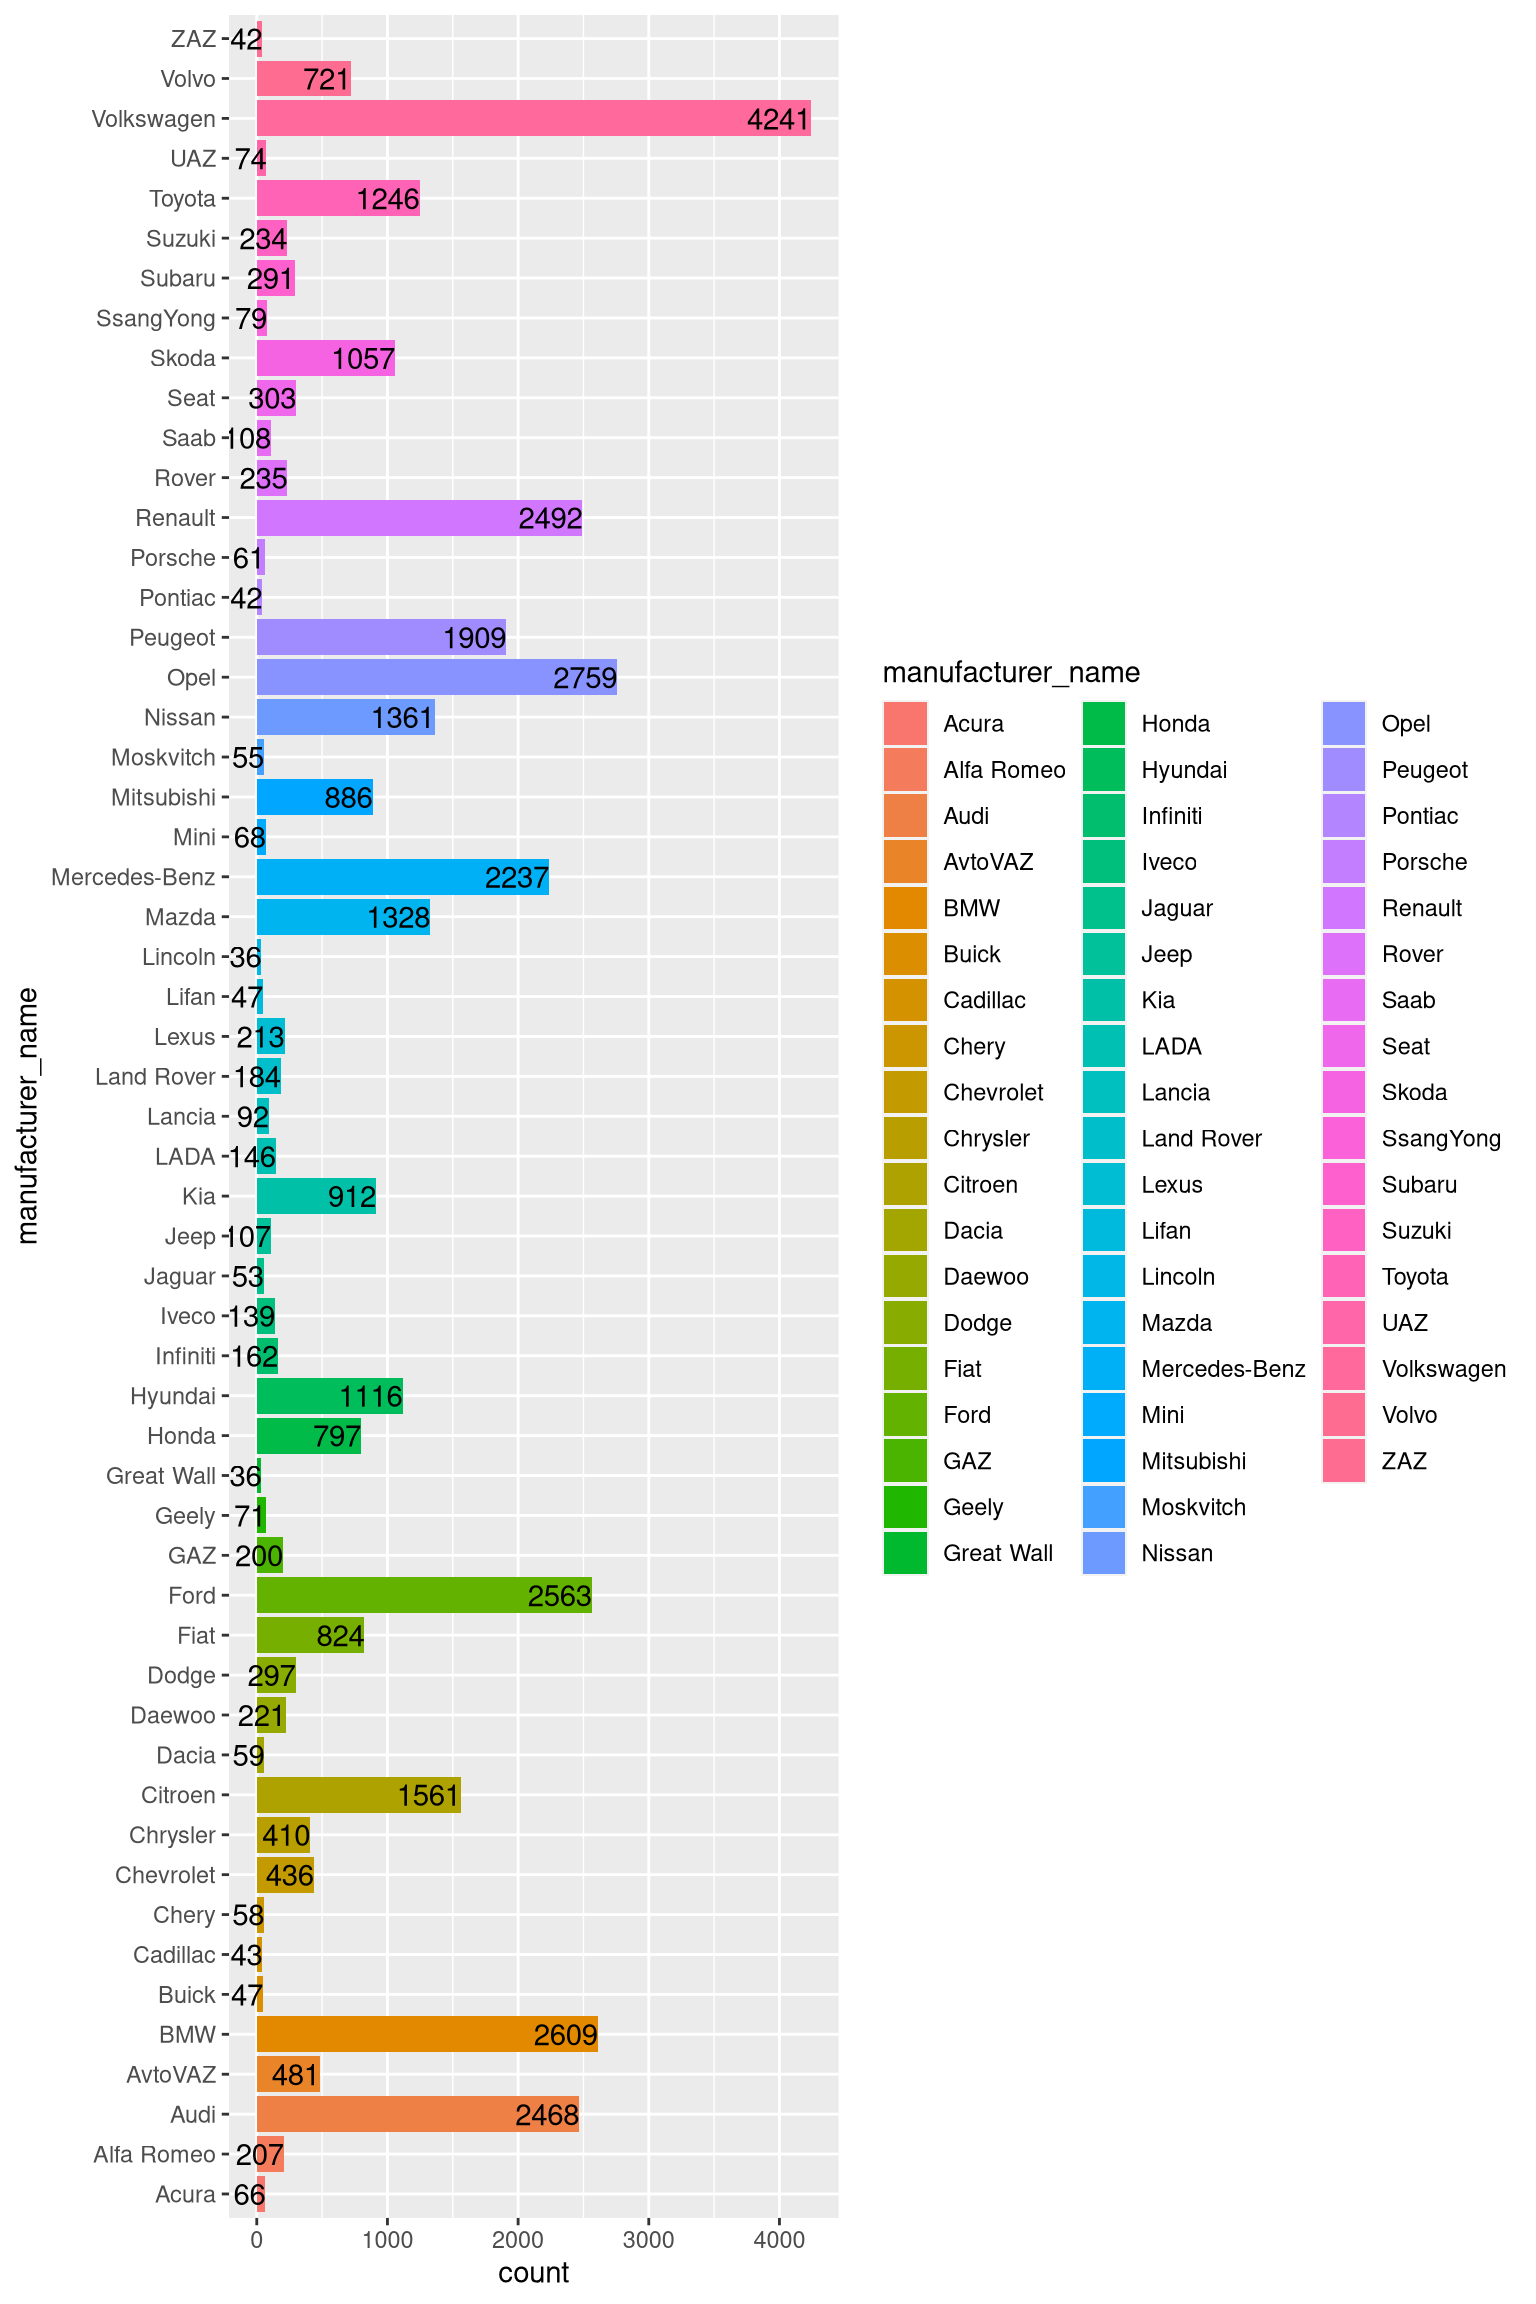
\includegraphics{Group1Report_files/figure-latex/ManDistrib-1.pdf}

We can see a large difference in the amount cars for each manufacturer.
Volkswagen, Opel, BMW, Audio, AvtoVAZ, Ford, Renault, and Mercedes-Benz
are the major manufacturers.

\begin{Shaded}
\begin{Highlighting}[]
\CommentTok{\# 2) A table to show unique car model names and quantity}
\NormalTok{cars\_edited }\SpecialCharTok{\%\textgreater{}\%} \FunctionTok{count}\NormalTok{(model\_name)}
\end{Highlighting}
\end{Shaded}

\begin{verbatim}
## # A tibble: 1,118 x 2
##    model_name     n
##    <chr>      <int>
##  1 <U+0410>21            8
##  2 <U+0410>22            3
##  3 <U+041C>20            6
##  4 <U+041C>5             4
##  5 100          371
##  6 1007           6
##  7 100NX          4
##  8 106           14
##  9 107           12
## 10 11             2
## # ... with 1,108 more rows
\end{verbatim}

\begin{Shaded}
\begin{Highlighting}[]
\CommentTok{\# 3) Plotting the number of cars with automatic or mechanical transmissions}
\NormalTok{transmissionGrouped }\OtherTok{\textless{}{-}} \FunctionTok{group\_by}\NormalTok{(cars\_edited, transmission)}
\NormalTok{transmissionCounted }\OtherTok{\textless{}{-}} \FunctionTok{count}\NormalTok{(transmissionGrouped)}
\NormalTok{percentTransmission }\OtherTok{\textless{}{-}} \FunctionTok{paste0}\NormalTok{(}\FunctionTok{round}\NormalTok{(}\DecValTok{100}\SpecialCharTok{*}\NormalTok{transmissionCounted}\SpecialCharTok{$}\NormalTok{n}\SpecialCharTok{/}\FunctionTok{sum}\NormalTok{(transmissionCounted}\SpecialCharTok{$}\NormalTok{n), }\DecValTok{2}\NormalTok{), }\StringTok{"\%"}\NormalTok{)}
\FunctionTok{pie}\NormalTok{(transmissionCounted}\SpecialCharTok{$}\NormalTok{n, }\AttributeTok{labels =}\NormalTok{ percentTransmission, }\AttributeTok{main =} \StringTok{"Transmission Distribution"}\NormalTok{, }\AttributeTok{col =} \FunctionTok{rainbow}\NormalTok{(}\FunctionTok{nrow}\NormalTok{(transmissionCounted)))}
\FunctionTok{legend}\NormalTok{(}\StringTok{"right"}\NormalTok{, }\FunctionTok{c}\NormalTok{(}\StringTok{"Automatic"}\NormalTok{, }\StringTok{"Mechanical"}\NormalTok{), }\AttributeTok{cex =} \FloatTok{0.8}\NormalTok{,}
       \AttributeTok{fill =} \FunctionTok{rainbow}\NormalTok{(}\FunctionTok{length}\NormalTok{(transmissionCounted)))}
\end{Highlighting}
\end{Shaded}

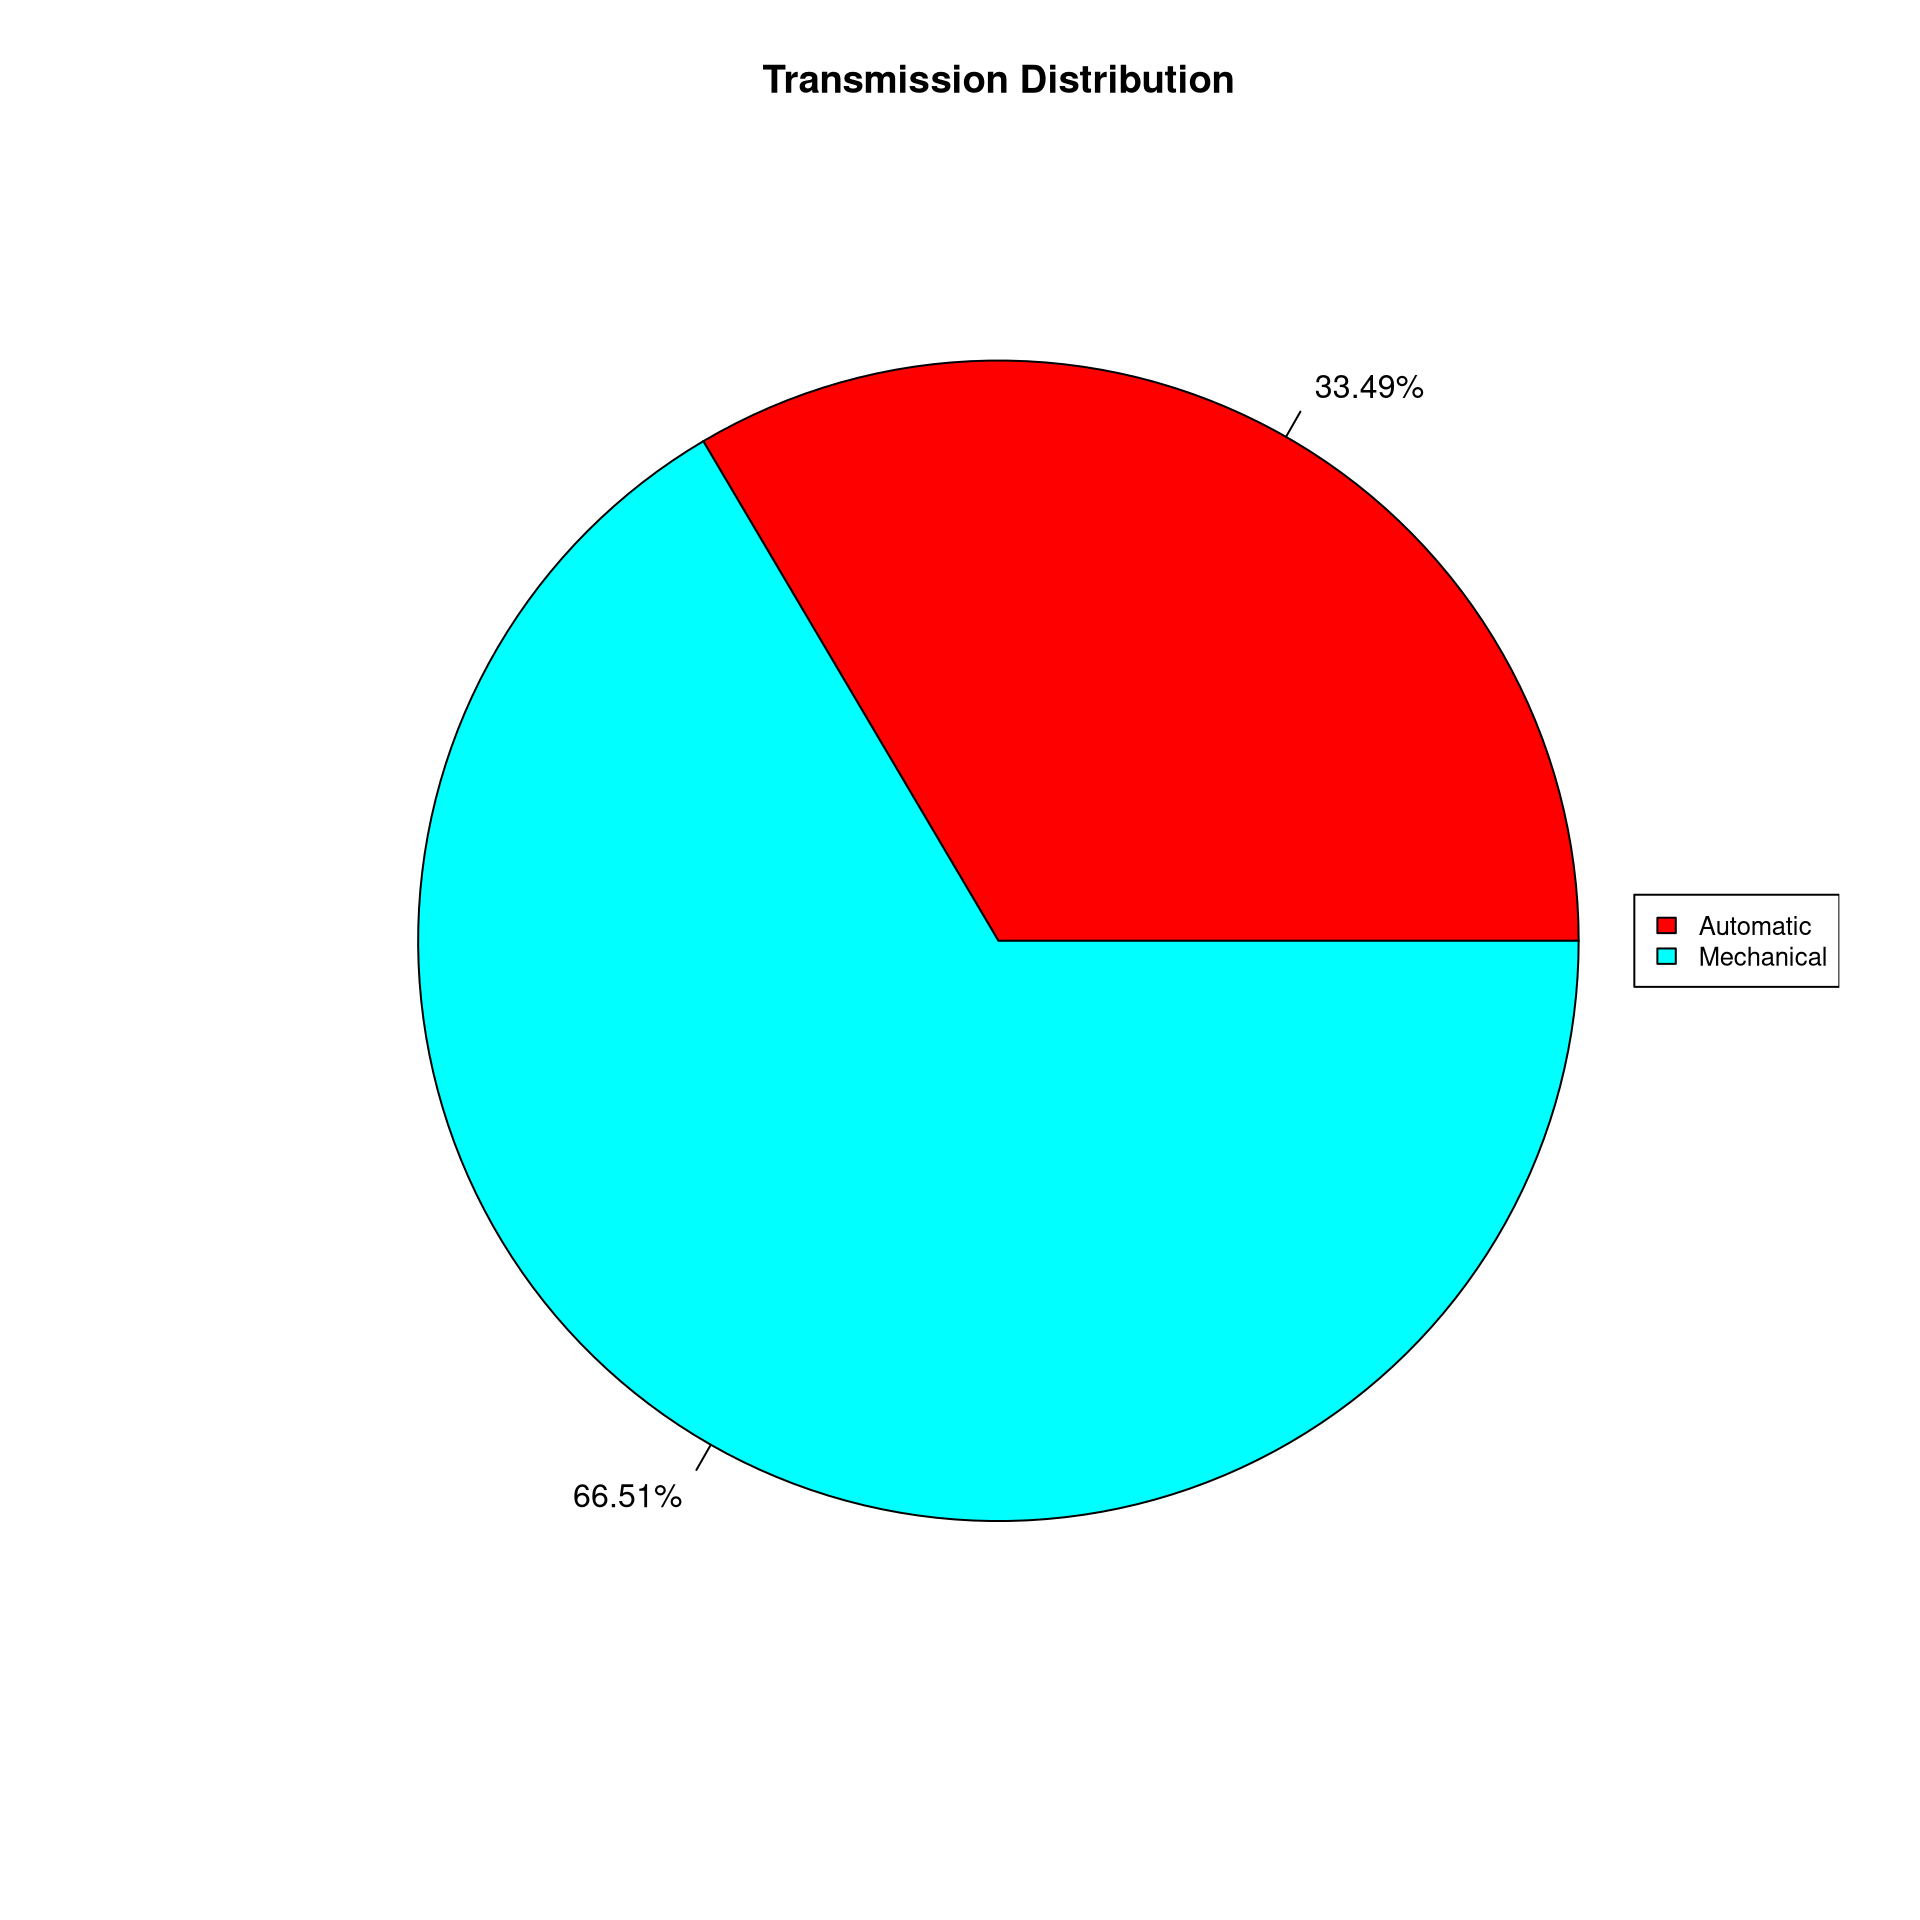
\includegraphics{Group1Report_files/figure-latex/TransmissionDistrib-1.pdf}

Mechanical is significantly more common than Automatic. This will be an
attribute to consider in our final model.

\begin{Shaded}
\begin{Highlighting}[]
\CommentTok{\# 4) Plotting cars by color and quantity}
\FunctionTok{ggplot}\NormalTok{(cars\_edited, }\FunctionTok{aes}\NormalTok{(}\AttributeTok{x =}\NormalTok{ color)) }\SpecialCharTok{+} \FunctionTok{geom\_bar}\NormalTok{(}\AttributeTok{stat =} \StringTok{"count"}\NormalTok{, }\FunctionTok{aes}\NormalTok{(}\AttributeTok{fill =}\NormalTok{ color)) }\SpecialCharTok{+} \FunctionTok{geom\_text}\NormalTok{(}\AttributeTok{stat =} \StringTok{"count"}\NormalTok{, }\FunctionTok{aes}\NormalTok{(}\AttributeTok{label =} \FunctionTok{after\_stat}\NormalTok{(count)), }\AttributeTok{vjust =} \SpecialCharTok{{-}}\DecValTok{1}\NormalTok{)}
\end{Highlighting}
\end{Shaded}

\includegraphics{Group1Report_files/figure-latex/ColorDistribution-1.pdf}

There is a lot of diversity in the colors and once again although there
are categories with more values there exists a decent amount of
variation.

\begin{Shaded}
\begin{Highlighting}[]
\CommentTok{\# 5) Histogram Odometer Value: Graph to see how the data is skewed}
\FunctionTok{ggplot}\NormalTok{(cars\_edited, }\FunctionTok{aes}\NormalTok{(odometer\_value)) }\SpecialCharTok{+} \FunctionTok{geom\_histogram}\NormalTok{()}
\end{Highlighting}
\end{Shaded}

\begin{verbatim}
## `stat_bin()` using `bins = 30`. Pick better value with `binwidth`.
\end{verbatim}

\includegraphics{Group1Report_files/figure-latex/OdometerDistribution-1.pdf}

The data is left-skewed with what appears to be outliers at around
1,000,000 miles.

\begin{Shaded}
\begin{Highlighting}[]
\CommentTok{\# 6) Histogram Year produced: Graph to see how the data is skewed}
\FunctionTok{ggplot}\NormalTok{(cars\_edited) }\SpecialCharTok{+} \FunctionTok{geom\_histogram}\NormalTok{(}\FunctionTok{aes}\NormalTok{(year\_produced))}
\end{Highlighting}
\end{Shaded}

\begin{verbatim}
## `stat_bin()` using `bins = 30`. Pick better value with `binwidth`.
\end{verbatim}

\includegraphics{Group1Report_files/figure-latex/YearProducedDistribution-1.pdf}

The graph seems to almost be normally distributed minus what appears to
be some outliers in the earlier years.

\begin{Shaded}
\begin{Highlighting}[]
\CommentTok{\# 7) Graph to show what fuel distribution}
\FunctionTok{ggplot}\NormalTok{(cars\_edited, }\FunctionTok{aes}\NormalTok{(}\AttributeTok{x =}\NormalTok{ engine\_fuel)) }\SpecialCharTok{+} \FunctionTok{geom\_bar}\NormalTok{(}\AttributeTok{stat =} \StringTok{"count"}\NormalTok{, }\FunctionTok{aes}\NormalTok{(}\AttributeTok{fill =}\NormalTok{ engine\_fuel)) }\SpecialCharTok{+} \FunctionTok{geom\_text}\NormalTok{(}\AttributeTok{stat =} \StringTok{"count"}\NormalTok{, }\FunctionTok{aes}\NormalTok{(}\AttributeTok{label =} \FunctionTok{after\_stat}\NormalTok{(count)), }\AttributeTok{vjust =} \SpecialCharTok{{-}}\DecValTok{1}\NormalTok{)}
\end{Highlighting}
\end{Shaded}

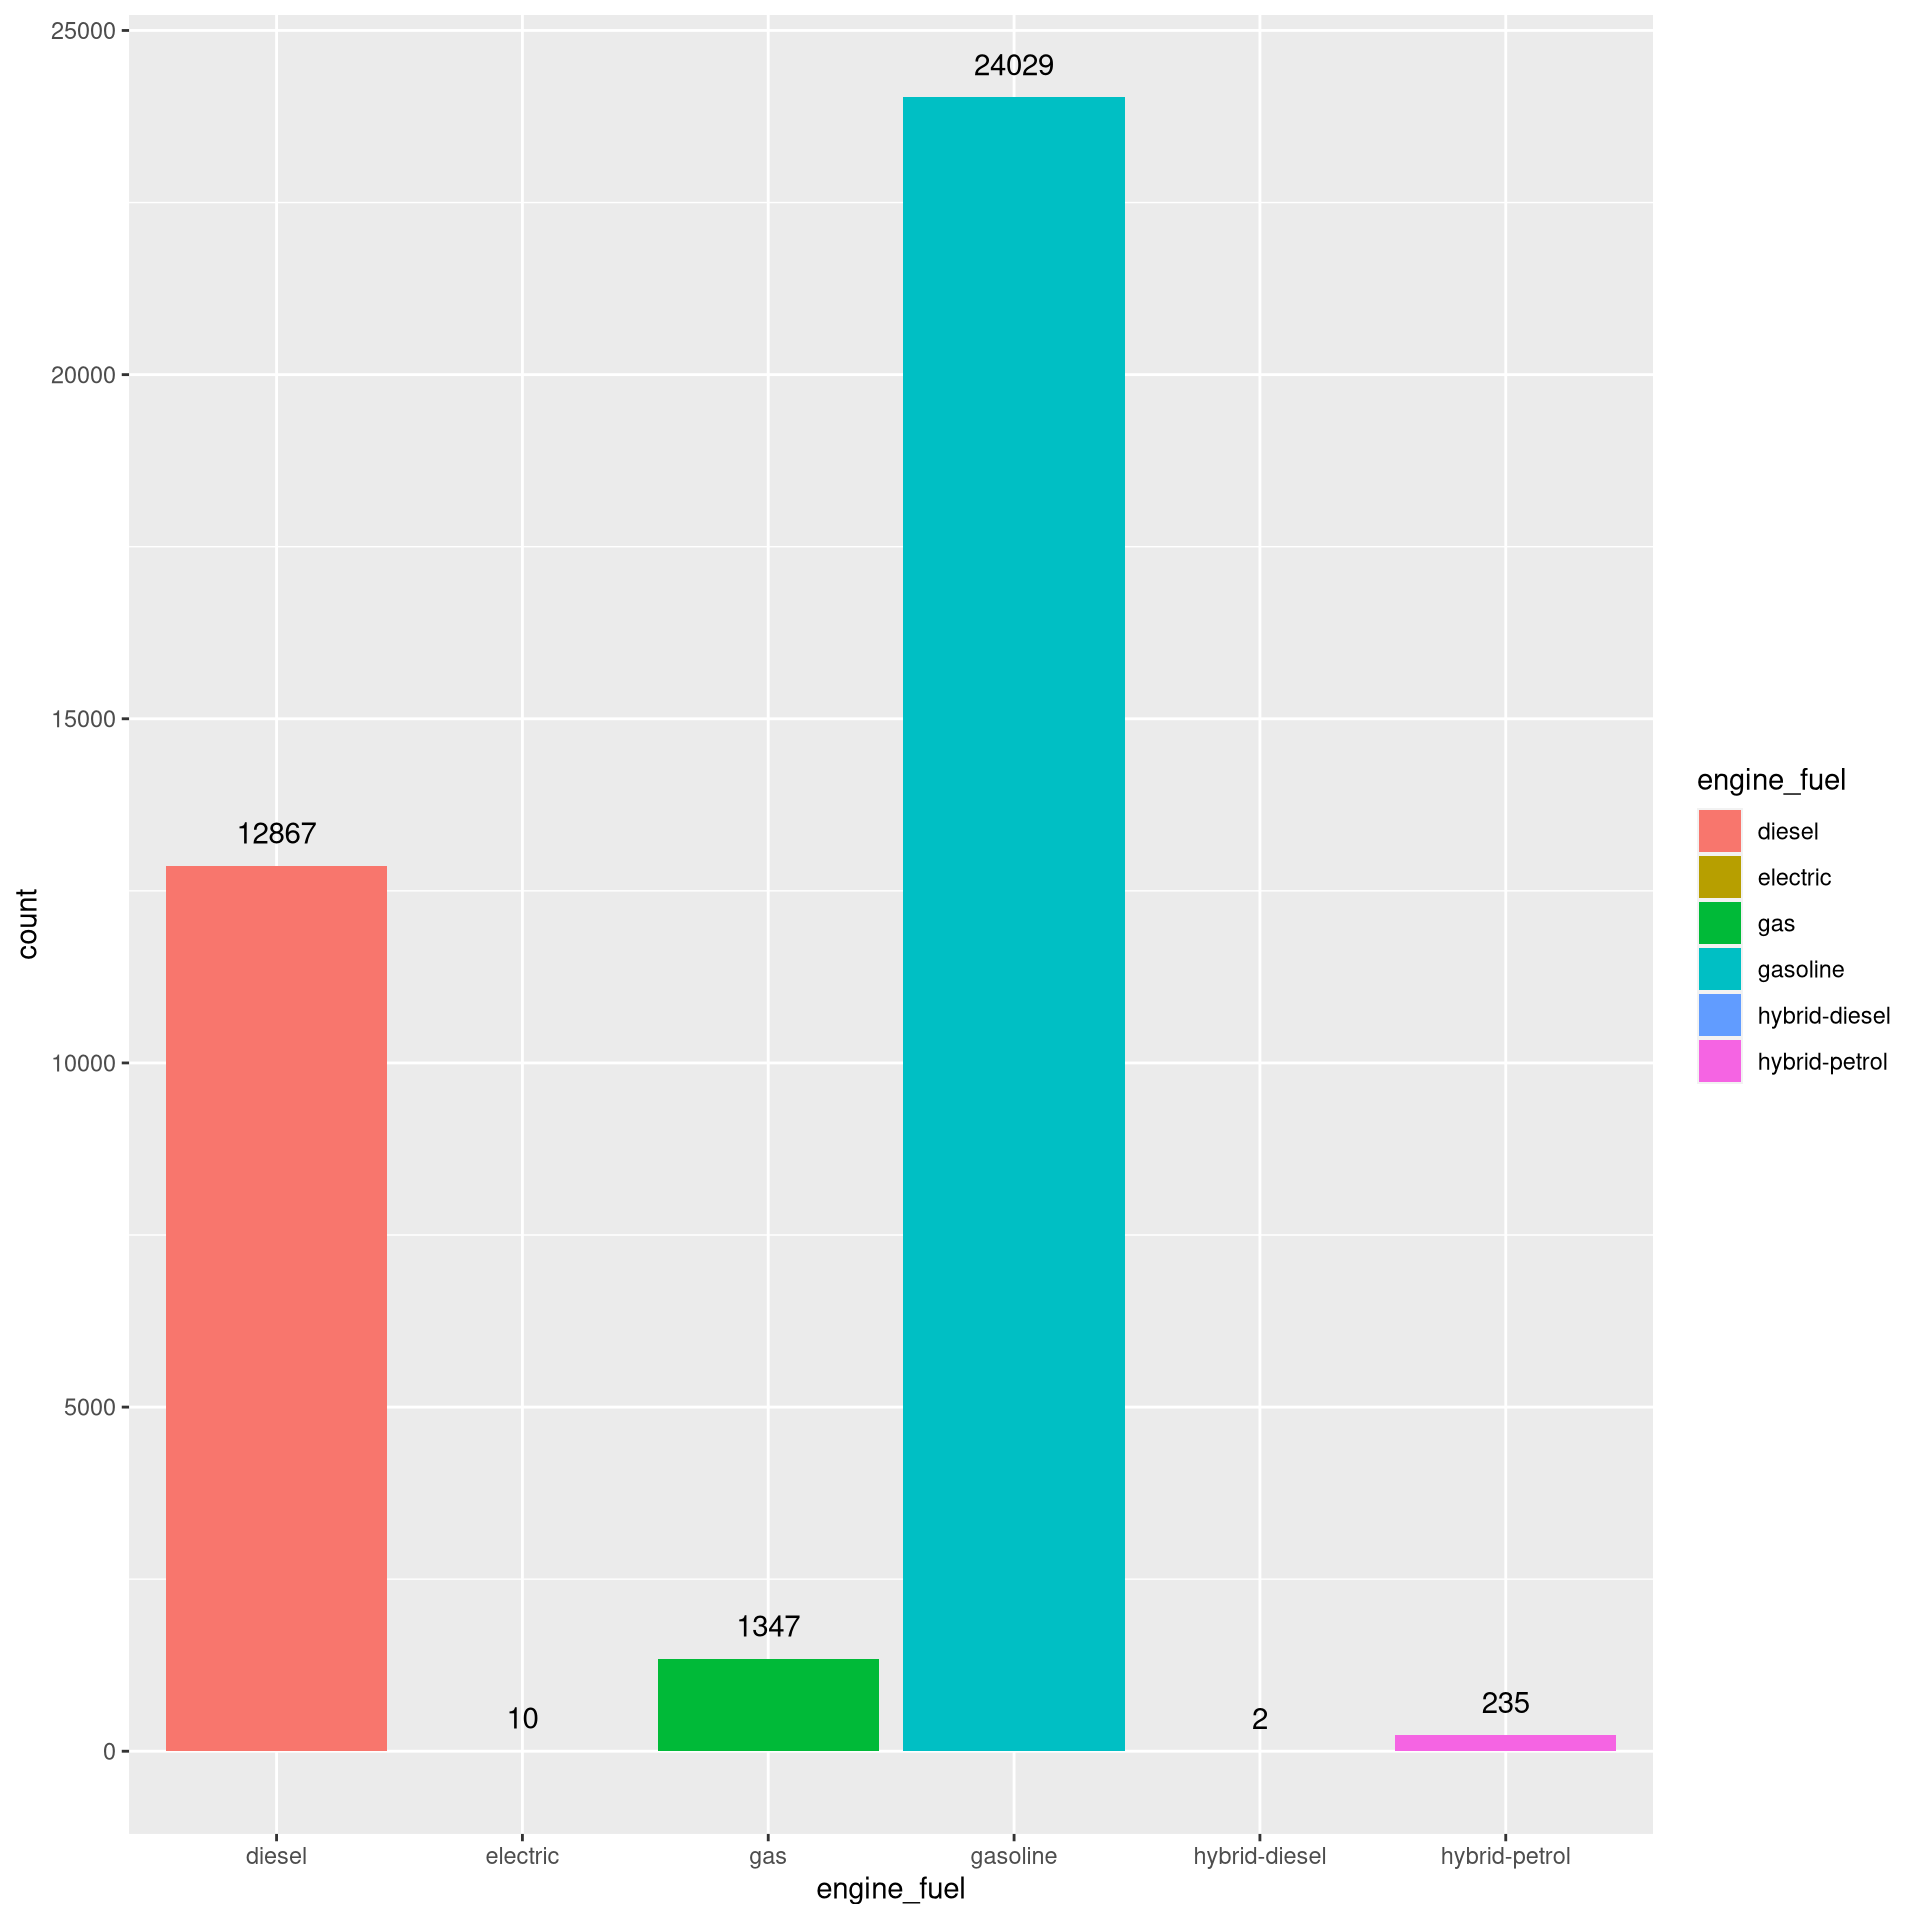
\includegraphics{Group1Report_files/figure-latex/FuelDistrib-1.pdf}

There are only 2 major engine fuels (gasoline and diesel).

\begin{Shaded}
\begin{Highlighting}[]
\CommentTok{\# 8) Pie graph to show engine type Distribution (Electric, Diesel, Gasoline)}
\NormalTok{TypeGrouped }\OtherTok{\textless{}{-}} \FunctionTok{group\_by}\NormalTok{(cars\_edited, engine\_type)}
\NormalTok{TypeCounted }\OtherTok{\textless{}{-}} \FunctionTok{count}\NormalTok{(TypeGrouped) }
\NormalTok{percentType }\OtherTok{\textless{}{-}} \FunctionTok{paste0}\NormalTok{(}\FunctionTok{round}\NormalTok{(}\DecValTok{100}\SpecialCharTok{*}\NormalTok{TypeCounted}\SpecialCharTok{$}\NormalTok{n}\SpecialCharTok{/}\FunctionTok{sum}\NormalTok{(TypeCounted}\SpecialCharTok{$}\NormalTok{n), }\DecValTok{2}\NormalTok{), }\StringTok{"\%"}\NormalTok{)}
\FunctionTok{pie}\NormalTok{(TypeCounted}\SpecialCharTok{$}\NormalTok{n, }\AttributeTok{labels =}\NormalTok{ percentType, }\AttributeTok{main =} \StringTok{"Engine Type Distribution"}\NormalTok{, }\AttributeTok{col =} \FunctionTok{rainbow}\NormalTok{(}\FunctionTok{nrow}\NormalTok{(TypeCounted)))}
\FunctionTok{legend}\NormalTok{(}\StringTok{"right"}\NormalTok{, }\FunctionTok{c}\NormalTok{(}\StringTok{"diesel"}\NormalTok{, }\StringTok{"electric"}\NormalTok{, }\StringTok{"gasoline"}\NormalTok{), }\AttributeTok{cex =} \FloatTok{0.8}\NormalTok{,}
       \AttributeTok{fill =} \FunctionTok{rainbow}\NormalTok{(}\FunctionTok{nrow}\NormalTok{(TypeCounted)))}
\end{Highlighting}
\end{Shaded}

\includegraphics{Group1Report_files/figure-latex/EngineDistrib-1.pdf}

Not surprisingly gasoline and diesel are the 2 most common Engine Type
considering the fuel distribution.

\begin{Shaded}
\begin{Highlighting}[]
\CommentTok{\# 9) Table for Engine capacity}
\NormalTok{cars\_edited }\SpecialCharTok{\%\textgreater{}\%} \FunctionTok{count}\NormalTok{(engine\_capacity)}
\end{Highlighting}
\end{Shaded}

\begin{verbatim}
## # A tibble: 62 x 2
##    engine_capacity     n
##              <dbl> <int>
##  1            -1      10
##  2             0.2     6
##  3             0.5     1
##  4             0.8    53
##  5             0.9    17
##  6             1     274
##  7             1.1   163
##  8             1.2   563
##  9             1.3   875
## 10             1.4  2393
## # ... with 52 more rows
\end{verbatim}

Engine Capacity seems to be left-skewed which may indicate outliers.

\begin{Shaded}
\begin{Highlighting}[]
\CommentTok{\# 10) Bar graph Body type: count how many cars have the same body type}
\FunctionTok{ggplot}\NormalTok{(cars\_edited, }\FunctionTok{aes}\NormalTok{(}\AttributeTok{x =}\NormalTok{ body\_type), }\AttributeTok{stat =} \StringTok{"count"}\NormalTok{) }\SpecialCharTok{+} \FunctionTok{geom\_bar}\NormalTok{() }\SpecialCharTok{+} \FunctionTok{geom\_text}\NormalTok{(}\AttributeTok{stat =} \StringTok{"count"}\NormalTok{, }\FunctionTok{aes}\NormalTok{(}\AttributeTok{label =} \FunctionTok{after\_stat}\NormalTok{(count)), }\AttributeTok{vjust =} \SpecialCharTok{{-}}\DecValTok{1}\NormalTok{)}
\end{Highlighting}
\end{Shaded}

\includegraphics{Group1Report_files/figure-latex/BodyTypeDistribution -1.pdf}

There is some diversity in body type and the diversity in categories may
lend itself to useful data for a future model.

\begin{Shaded}
\begin{Highlighting}[]
\CommentTok{\# 11) Graph Drivetrain distribution:}
\NormalTok{drivetrainGrouped }\OtherTok{\textless{}{-}} \FunctionTok{group\_by}\NormalTok{(cars\_edited, drivetrain)}
\NormalTok{drivetrainCounted }\OtherTok{\textless{}{-}} \FunctionTok{count}\NormalTok{(drivetrainGrouped) }
\NormalTok{percentdrivetrain }\OtherTok{\textless{}{-}} \FunctionTok{paste0}\NormalTok{(}\FunctionTok{round}\NormalTok{(}\DecValTok{100}\SpecialCharTok{*}\NormalTok{drivetrainCounted}\SpecialCharTok{$}\NormalTok{n}\SpecialCharTok{/}\FunctionTok{sum}\NormalTok{(drivetrainCounted}\SpecialCharTok{$}\NormalTok{n), }\DecValTok{2}\NormalTok{), }\StringTok{"\%"}\NormalTok{)}
\FunctionTok{pie}\NormalTok{(drivetrainCounted}\SpecialCharTok{$}\NormalTok{n, }\AttributeTok{labels =}\NormalTok{ percentdrivetrain, }\AttributeTok{main =} \StringTok{"Drivetrain Distribution"}\NormalTok{, }\AttributeTok{col =} \FunctionTok{rainbow}\NormalTok{(}\FunctionTok{nrow}\NormalTok{(drivetrainCounted)))}
\FunctionTok{legend}\NormalTok{(}\StringTok{"right"}\NormalTok{, }\FunctionTok{c}\NormalTok{(}\StringTok{"all"}\NormalTok{, }\StringTok{"front"}\NormalTok{, }\StringTok{"rear"}\NormalTok{), }\AttributeTok{cex =} \FloatTok{0.8}\NormalTok{,}
       \AttributeTok{fill =} \FunctionTok{rainbow}\NormalTok{(}\FunctionTok{nrow}\NormalTok{(drivetrainCounted)))}
\end{Highlighting}
\end{Shaded}

\includegraphics{Group1Report_files/figure-latex/DrivetrainDistribution -1.pdf}

Although most vehicles are front wheel drive there is enough all and
real wheel drive to gather some promising insights.

\begin{Shaded}
\begin{Highlighting}[]
\CommentTok{\# 12) Number of cars with same price}
\FunctionTok{ggplot}\NormalTok{(cars\_edited, }\FunctionTok{aes}\NormalTok{(}\AttributeTok{x =}\NormalTok{ price\_usd), }\AttributeTok{stat =} \StringTok{"count"}\NormalTok{) }\SpecialCharTok{+} \FunctionTok{geom\_histogram}\NormalTok{()}
\end{Highlighting}
\end{Shaded}

\begin{verbatim}
## `stat_bin()` using `bins = 30`. Pick better value with `binwidth`.
\end{verbatim}

\includegraphics{Group1Report_files/figure-latex/PriceDistribution -1.pdf}

This graph is extremely left-skewed. The sheer usefulness of price in
our dataset will make this our main response attribute.

\begin{Shaded}
\begin{Highlighting}[]
\CommentTok{\# 13) Pie Graph exchangeability Distribution}
\NormalTok{exchangeableGrouped }\OtherTok{\textless{}{-}} \FunctionTok{group\_by}\NormalTok{(cars\_edited, is\_exchangeable)}
\NormalTok{exchangeableCounted }\OtherTok{\textless{}{-}} \FunctionTok{count}\NormalTok{(exchangeableGrouped) }
\NormalTok{percentexchangeable }\OtherTok{\textless{}{-}} \FunctionTok{paste0}\NormalTok{(}\FunctionTok{round}\NormalTok{(}\DecValTok{100}\SpecialCharTok{*}\NormalTok{exchangeableCounted}\SpecialCharTok{$}\NormalTok{n}\SpecialCharTok{/}\FunctionTok{sum}\NormalTok{(exchangeableCounted}\SpecialCharTok{$}\NormalTok{n), }\DecValTok{2}\NormalTok{), }\StringTok{"\%"}\NormalTok{)}
\FunctionTok{pie}\NormalTok{(exchangeableCounted}\SpecialCharTok{$}\NormalTok{n, }\AttributeTok{labels =}\NormalTok{ percentexchangeable, }\AttributeTok{main =} \StringTok{"Exchangeability Distribution"}\NormalTok{, }\AttributeTok{col =} \FunctionTok{rainbow}\NormalTok{(}\FunctionTok{nrow}\NormalTok{(exchangeableCounted)))}
\FunctionTok{legend}\NormalTok{(}\StringTok{"right"}\NormalTok{, }\FunctionTok{c}\NormalTok{(}\StringTok{"False"}\NormalTok{, }\StringTok{"True"}\NormalTok{), }\AttributeTok{cex =} \FloatTok{0.8}\NormalTok{,}
       \AttributeTok{fill =} \FunctionTok{rainbow}\NormalTok{(}\FunctionTok{nrow}\NormalTok{(exchangeableCounted)))}
\end{Highlighting}
\end{Shaded}

\includegraphics{Group1Report_files/figure-latex/ExchangebilityDistribution -1.pdf}

Exchangeability is more common than anticipated. It will be interesting
to see if pricier or cheaper cars consent to exchanges.

\begin{Shaded}
\begin{Highlighting}[]
\CommentTok{\# 14) Pie Graph Location region: Count the number of cars in a region}
\NormalTok{regionPriceDF }\OtherTok{\textless{}{-}} \FunctionTok{group\_by}\NormalTok{(cars\_edited, location\_region)}
\NormalTok{regionPriceDFCount }\OtherTok{\textless{}{-}} \FunctionTok{count}\NormalTok{(regionPriceDF)}
\NormalTok{percentRegion }\OtherTok{\textless{}{-}} \FunctionTok{paste0}\NormalTok{(}\FunctionTok{round}\NormalTok{(}\DecValTok{100}\SpecialCharTok{*}\NormalTok{regionPriceDFCount}\SpecialCharTok{$}\NormalTok{n}\SpecialCharTok{/}\FunctionTok{sum}\NormalTok{(regionPriceDFCount}\SpecialCharTok{$}\NormalTok{n), }\DecValTok{2}\NormalTok{), }\StringTok{"\%"}\NormalTok{)}
\FunctionTok{pie}\NormalTok{(regionPriceDFCount}\SpecialCharTok{$}\NormalTok{n, }\AttributeTok{labels =}\NormalTok{ percentRegion, }\AttributeTok{main =} \StringTok{"Region Price Distribution"}\NormalTok{, }\AttributeTok{col =} \FunctionTok{rainbow}\NormalTok{(}\FunctionTok{nrow}\NormalTok{(regionPriceDFCount)))}
\FunctionTok{legend}\NormalTok{(}\StringTok{"right"}\NormalTok{, }\FunctionTok{c}\NormalTok{(}\StringTok{"Brest Region"}\NormalTok{, }\StringTok{"Gomel Region"}\NormalTok{, }\StringTok{"Grodno Region"}\NormalTok{, }\StringTok{"Minsk Region"}\NormalTok{, }\StringTok{"Mogilev Region"}\NormalTok{, }\StringTok{"Vitebsk Region"}\NormalTok{), }\AttributeTok{cex =} \FloatTok{0.8}\NormalTok{,}
       \AttributeTok{fill =} \FunctionTok{rainbow}\NormalTok{(}\FunctionTok{nrow}\NormalTok{(regionPriceDFCount)))}
\end{Highlighting}
\end{Shaded}

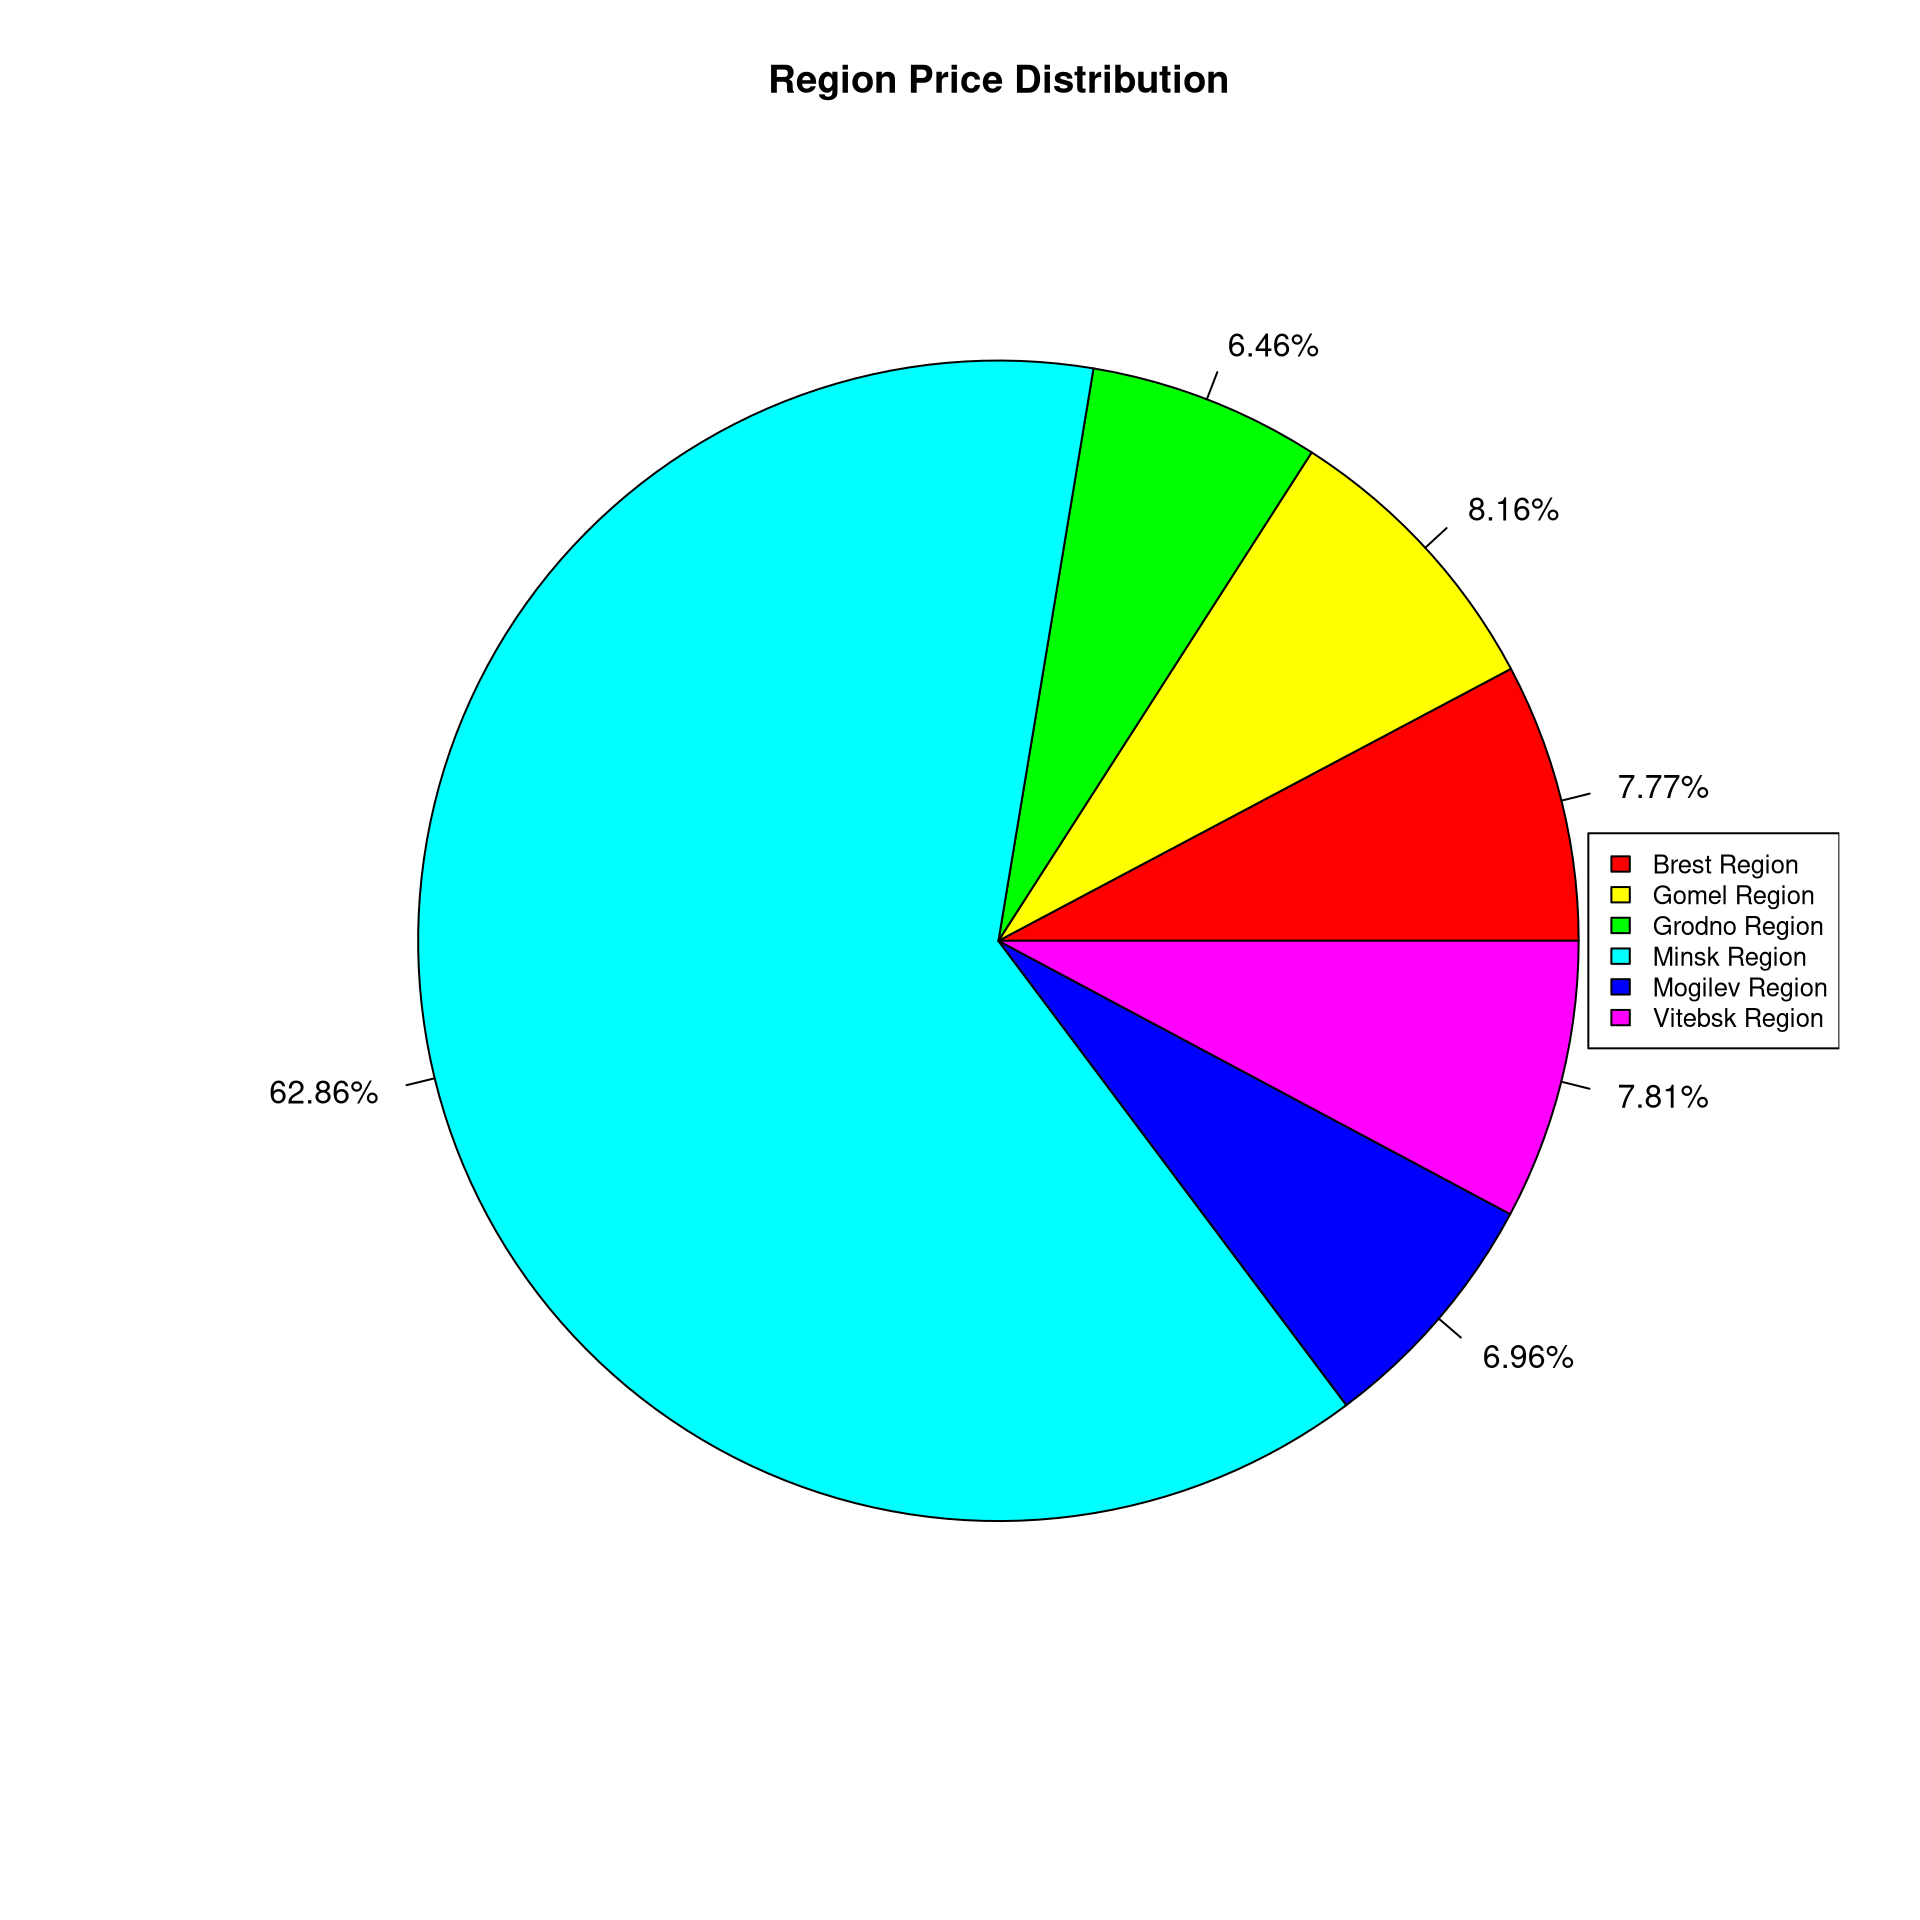
\includegraphics{Group1Report_files/figure-latex/RegionDistrib-1.pdf}

Minsk accounts for a very large number of vehicles (makes sense
considering the population sizes) with even distributions everywhere
else. The usefulness of the attribute may be less since Minsk is such a
large portion of the data.

\begin{Shaded}
\begin{Highlighting}[]
\CommentTok{\# 15) Histogram Number of photos: Graph to see how the data is skewed}
\FunctionTok{ggplot}\NormalTok{(cars\_edited) }\SpecialCharTok{+} \FunctionTok{geom\_histogram}\NormalTok{(}\AttributeTok{mapping =} \FunctionTok{aes}\NormalTok{(number\_of\_photos))}
\end{Highlighting}
\end{Shaded}

\begin{verbatim}
## `stat_bin()` using `bins = 30`. Pick better value with `binwidth`.
\end{verbatim}

\includegraphics{Group1Report_files/figure-latex/NumPhotosHistogram-1.pdf}

The graph is very left-skewed. I suspect photos may increase the value
of a vehicle, but tests will need to be done to affirm this.

\begin{Shaded}
\begin{Highlighting}[]
\CommentTok{\# 16) Box plot Number of photos: Graph to see how the data is skewed}
\FunctionTok{ggplot}\NormalTok{(cars\_edited) }\SpecialCharTok{+} \FunctionTok{geom\_boxplot}\NormalTok{(}\AttributeTok{mapping =} \FunctionTok{aes}\NormalTok{(number\_of\_photos))}
\end{Highlighting}
\end{Shaded}

\includegraphics{Group1Report_files/figure-latex/NumPhotosBoxplot-1.pdf}

There are many outliers. With extra time we may be able to investigate
the impact of these outliers on the data.

\begin{Shaded}
\begin{Highlighting}[]
\CommentTok{\# 17) Histogram Up counter: investigating how our outliers look with our modifications}
\FunctionTok{ggplot}\NormalTok{(cars\_edited) }\SpecialCharTok{+} \FunctionTok{geom\_histogram}\NormalTok{(}\AttributeTok{mapping =} \FunctionTok{aes}\NormalTok{(up\_counter))}
\end{Highlighting}
\end{Shaded}

\begin{verbatim}
## `stat_bin()` using `bins = 30`. Pick better value with `binwidth`.
\end{verbatim}

\includegraphics{Group1Report_files/figure-latex/Up CounterHistogram-1.pdf}

Clearly an outlier exists since there is a large scale.

\begin{Shaded}
\begin{Highlighting}[]
\CommentTok{\# 18) Box plot Duration listed: investigating how our outliers look with our modifications}
\FunctionTok{ggplot}\NormalTok{(cars\_edited) }\SpecialCharTok{+} \FunctionTok{geom\_boxplot}\NormalTok{(}\AttributeTok{mapping =} \FunctionTok{aes}\NormalTok{(duration\_listed))}
\end{Highlighting}
\end{Shaded}

\includegraphics{Group1Report_files/figure-latex/DurationBoxplot-1.pdf}

There is a significant number of outliers. There is no evidence to
conclude these should be eliminated.

\begin{Shaded}
\begin{Highlighting}[]
\CommentTok{\# 19) Histogram Duration listed: Graph to see how the data is skewed}
\FunctionTok{ggplot}\NormalTok{(cars\_edited) }\SpecialCharTok{+} \FunctionTok{geom\_histogram}\NormalTok{(}\FunctionTok{aes}\NormalTok{(duration\_listed))}
\end{Highlighting}
\end{Shaded}

\begin{verbatim}
## `stat_bin()` using `bins = 30`. Pick better value with `binwidth`.
\end{verbatim}

\includegraphics{Group1Report_files/figure-latex/DurationHistogram-1.pdf}

The histogram shows a skew in the duration listing for our dataset.

Once a general understanding of each attribute was gained, we began to
visualize various combinations of attributions. These visualizations
were vital in seeing different relationships among our samples. The
visualizations that were used were Balloon Plot, Scatterplot, frequency
polygons, dplyr::summarize, and Boxplots.

\begin{Shaded}
\begin{Highlighting}[]
\CommentTok{\# 1) Graph to show the number of cars(by manufacturer name) in a region BALLOON PLOT}
\FunctionTok{ggplot}\NormalTok{(cars\_edited, }\FunctionTok{aes}\NormalTok{(location\_region, manufacturer\_name)) }\SpecialCharTok{+} \FunctionTok{geom\_count}\NormalTok{()}
\end{Highlighting}
\end{Shaded}

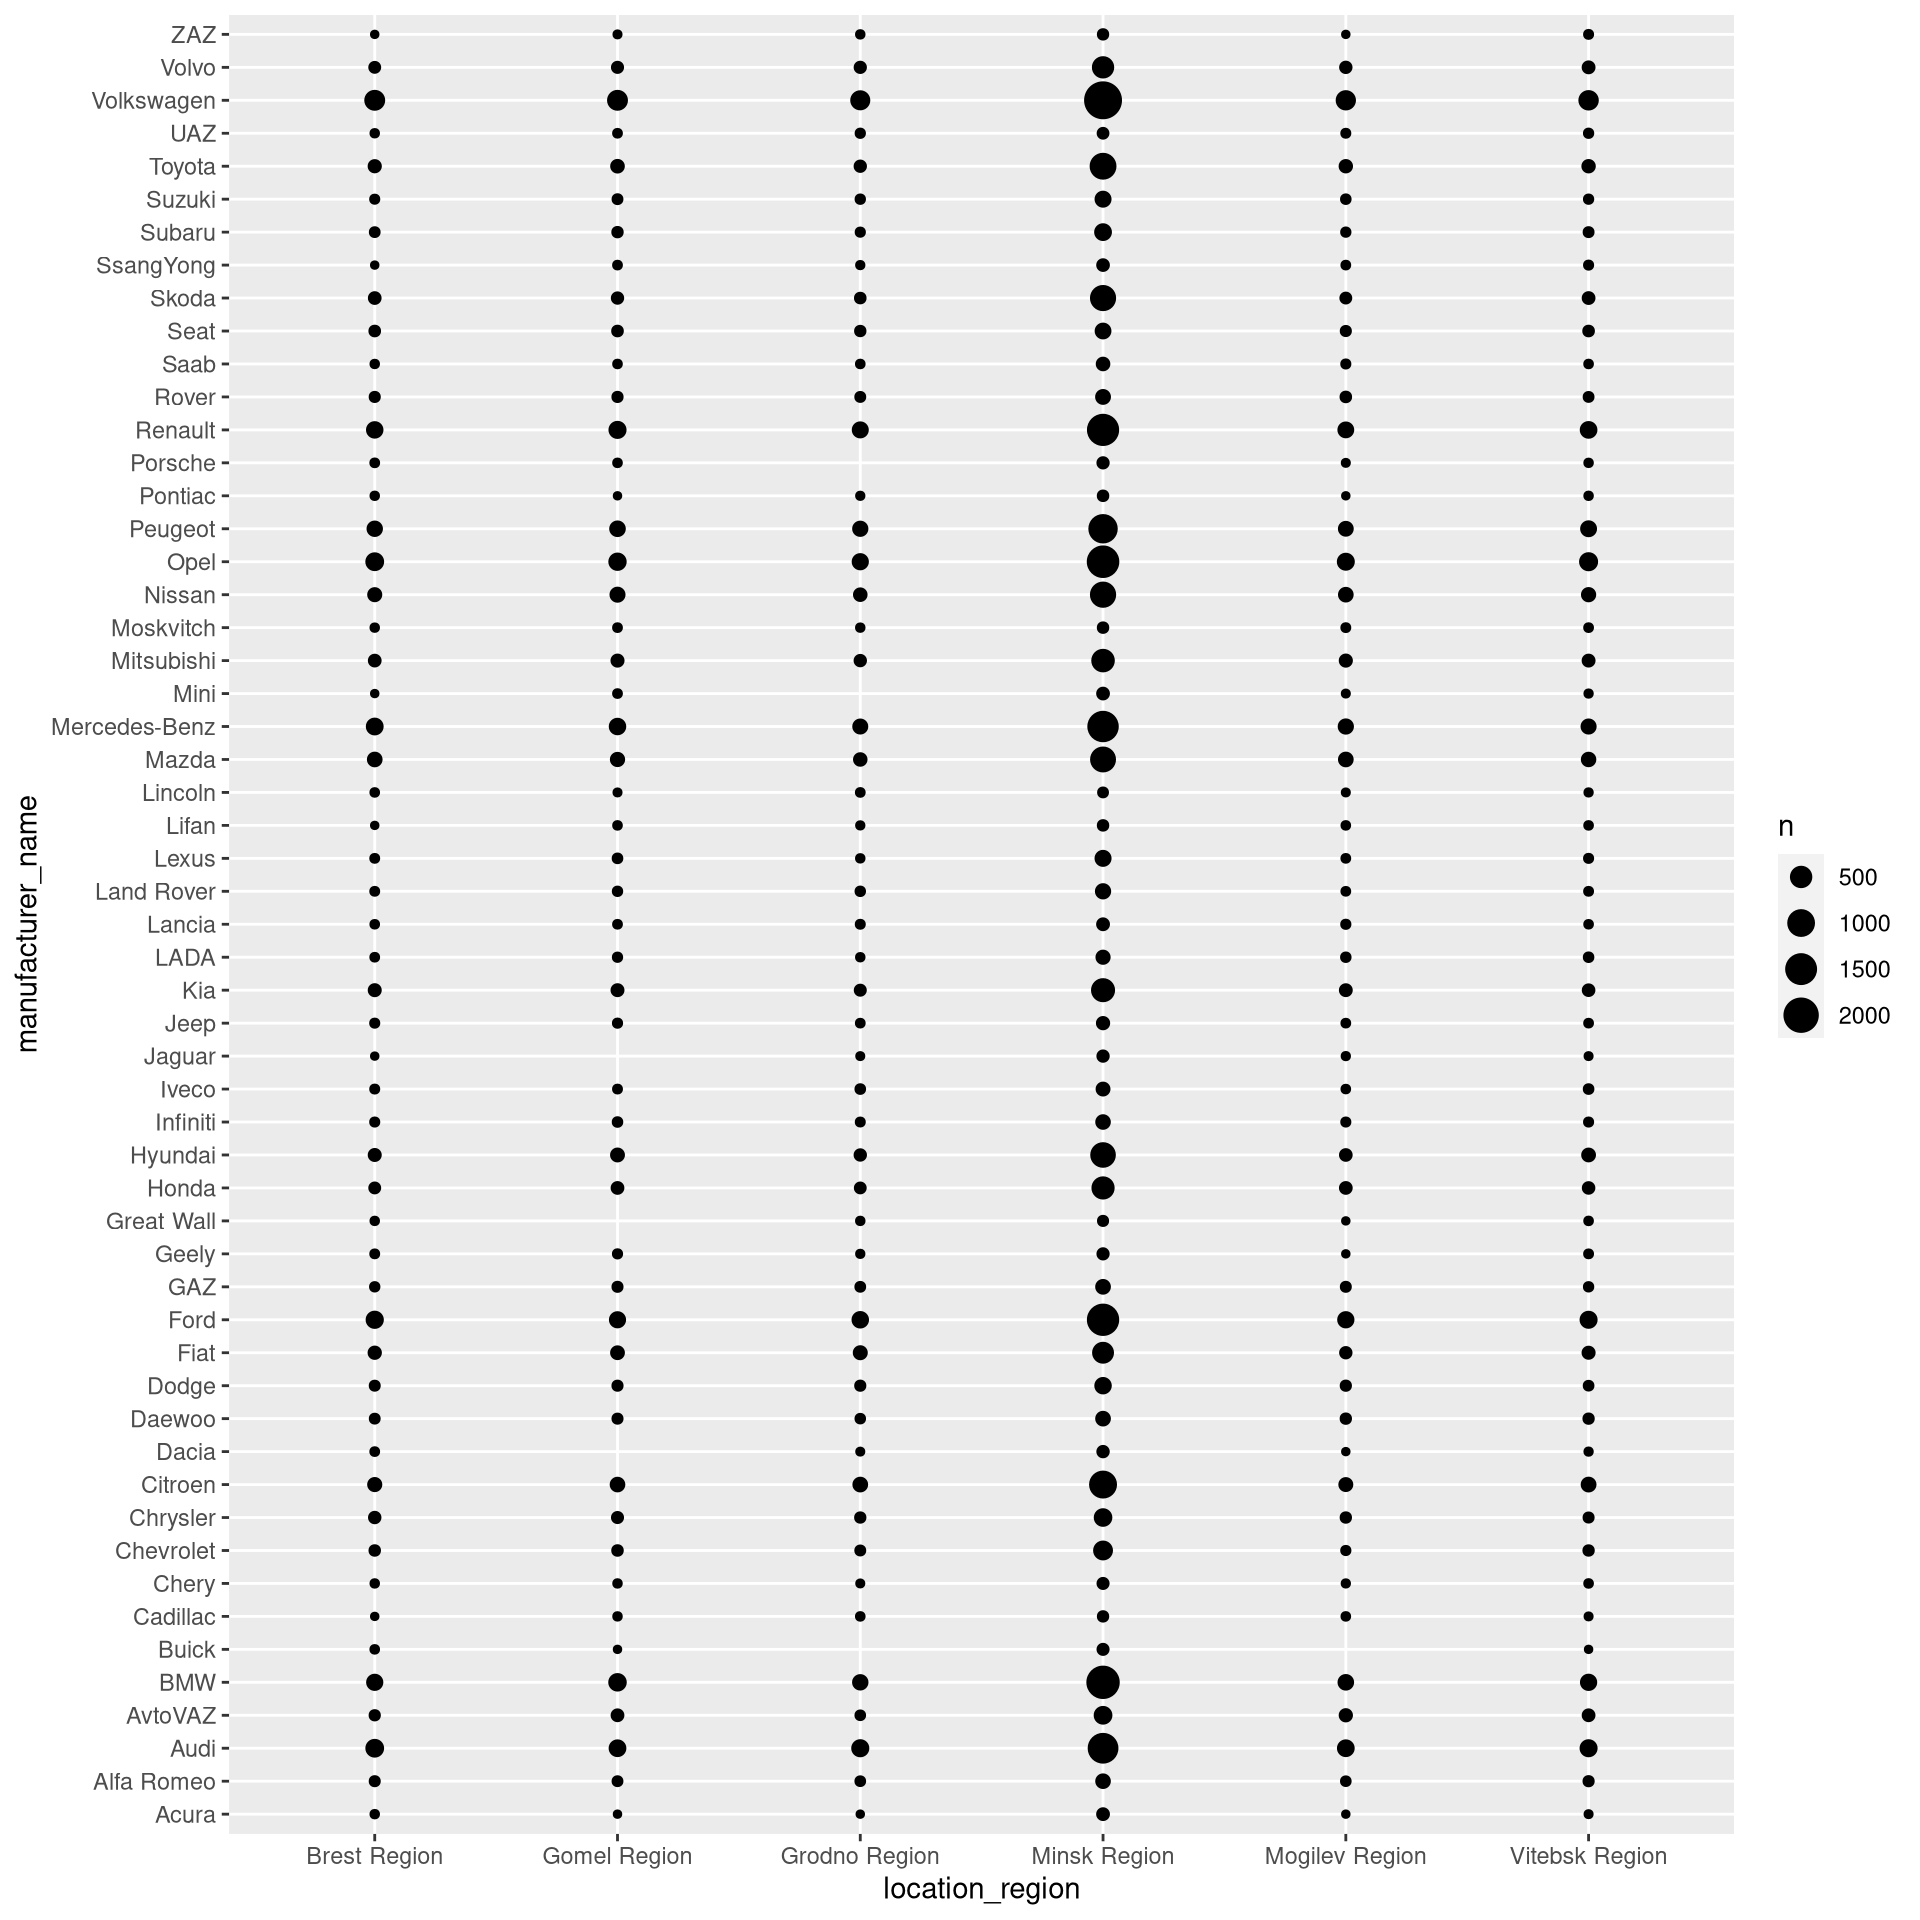
\includegraphics{Group1Report_files/figure-latex/ManufByRegion-1.pdf}

Due to the quantity of categories a test will need to be done to gather
significant data.

\begin{Shaded}
\begin{Highlighting}[]
\CommentTok{\# 2) Graph to show the price of a car according to its year produced SCATTER PLOT}
\FunctionTok{ggplot}\NormalTok{(cars\_edited, }\FunctionTok{aes}\NormalTok{(year\_produced, price\_usd)) }\SpecialCharTok{+} \FunctionTok{geom\_point}\NormalTok{() }\SpecialCharTok{+} \FunctionTok{geom\_smooth}\NormalTok{()}
\end{Highlighting}
\end{Shaded}

\begin{verbatim}
## `geom_smooth()` using method = 'gam' and formula 'y ~ s(x, bs = "cs")'
\end{verbatim}

\includegraphics{Group1Report_files/figure-latex/PriceByYear-1.pdf}

There exists a parabolic relationship between year\_produced and
price\_usd.

\begin{Shaded}
\begin{Highlighting}[]
\CommentTok{\# 3) Graph to show the number of cars in specific colors(10 red cars, 8 blue cars etc.) by region BAR GRAPH}
\FunctionTok{ggplot}\NormalTok{(cars\_edited, }\FunctionTok{aes}\NormalTok{(color)) }\SpecialCharTok{+} \FunctionTok{geom\_bar}\NormalTok{(}\FunctionTok{aes}\NormalTok{(}\AttributeTok{fill =}\NormalTok{ location\_region))}
\end{Highlighting}
\end{Shaded}

\includegraphics{Group1Report_files/figure-latex/CarsByColor-1.pdf}

From looking at the bar graph there does not seem to be any significant
differences in color distribution for locations.

\begin{Shaded}
\begin{Highlighting}[]
\CommentTok{\# 4) Graph to show the price of a car according to its millage(odometer) SCATTER PLOT}
\FunctionTok{ggplot}\NormalTok{(cars\_edited, }\FunctionTok{aes}\NormalTok{(odometer\_value, price\_usd)) }\SpecialCharTok{+} \FunctionTok{geom\_point}\NormalTok{(}\FunctionTok{aes}\NormalTok{(}\AttributeTok{color =}\NormalTok{ is\_exchangeable)) }\SpecialCharTok{+} \FunctionTok{geom\_smooth}\NormalTok{()}
\end{Highlighting}
\end{Shaded}

\begin{verbatim}
## `geom_smooth()` using method = 'gam' and formula 'y ~ s(x, bs = "cs")'
\end{verbatim}

\includegraphics{Group1Report_files/figure-latex/CarsByOdometerandExchangeable-1.pdf}

This graph is incredibly diverse and indicates that there is a need for
advanced models to access price relationships.

\begin{Shaded}
\begin{Highlighting}[]
\CommentTok{\# 5)Graph to show the price of a car according to its year produced AND body type SCATTER PLOT}
\FunctionTok{ggplot}\NormalTok{(cars\_edited, }\FunctionTok{aes}\NormalTok{(year\_produced, price\_usd)) }\SpecialCharTok{+} \FunctionTok{geom\_point}\NormalTok{(}\FunctionTok{aes}\NormalTok{(}\AttributeTok{color =}\NormalTok{ body\_type)) }\SpecialCharTok{+} \FunctionTok{geom\_smooth}\NormalTok{()}
\end{Highlighting}
\end{Shaded}

\begin{verbatim}
## `geom_smooth()` using method = 'gam' and formula 'y ~ s(x, bs = "cs")'
\end{verbatim}

\includegraphics{Group1Report_files/figure-latex/PriceByYearAndType-1.pdf}

The quantity of samples makes this graph hard to dissect. One would have
to perform tests to see how body type relates to price.

\begin{Shaded}
\begin{Highlighting}[]
\CommentTok{\# 6) Group by car body type and get its mean price}
\FunctionTok{group\_by}\NormalTok{(cars\_edited, body\_type) }\SpecialCharTok{\%\textgreater{}\%} \FunctionTok{summarise}\NormalTok{(}\AttributeTok{price\_mean =} \FunctionTok{mean}\NormalTok{(price\_usd))}
\end{Highlighting}
\end{Shaded}

\begin{verbatim}
## # A tibble: 12 x 2
##    body_type price_mean
##    <chr>          <dbl>
##  1 cabriolet     10976.
##  2 coupe          7458.
##  3 hatchback      4036.
##  4 liftback       7873.
##  5 limousine      8154.
##  6 minibus        8466.
##  7 minivan        6131.
##  8 pickup        11748.
##  9 sedan          5782.
## 10 suv           13768.
## 11 universal      5017.
## 12 van            6675.
\end{verbatim}

\begin{Shaded}
\begin{Highlighting}[]
\CommentTok{\# 7) Graph to show the outliers with body type and price BOX PLOT}
\FunctionTok{ggplot}\NormalTok{(cars\_edited) }\SpecialCharTok{+} \FunctionTok{geom\_boxplot}\NormalTok{(}\AttributeTok{mapping =} \FunctionTok{aes}\NormalTok{(}\AttributeTok{x =} \FunctionTok{reorder}\NormalTok{(body\_type, price\_usd), }\AttributeTok{y =}
\NormalTok{                                                   price\_usd))}
\end{Highlighting}
\end{Shaded}

\includegraphics{Group1Report_files/figure-latex/BodyTypeAndPriceboxplot-1.pdf}

This graph tells us that given more time it may be useful to test our
models without outliers.

\begin{Shaded}
\begin{Highlighting}[]
\CommentTok{\# 8) Graph to show the correlation between car body type, price, AND engine fuel}
\FunctionTok{ggplot}\NormalTok{(cars\_edited) }\SpecialCharTok{+} \FunctionTok{geom\_point}\NormalTok{(}\AttributeTok{mapping =} \FunctionTok{aes}\NormalTok{(}\AttributeTok{x =}\NormalTok{ body\_type, }\AttributeTok{y =}\NormalTok{ price\_usd, }\AttributeTok{color =}\NormalTok{ engine\_fuel))}
\end{Highlighting}
\end{Shaded}

\includegraphics{Group1Report_files/figure-latex/BodyTypePriceAndEngineFuel-1.pdf}

This graph tells us that certain body types tend to come with engines
for specific fuels. The range for prices seems to be very scattered.

\begin{Shaded}
\begin{Highlighting}[]
\CommentTok{\# 9) Graph to show the price of a car according to its number of photos incl. engine fuel SCATTER PLOT}
\FunctionTok{ggplot}\NormalTok{(cars\_edited) }\SpecialCharTok{+} \FunctionTok{geom\_point}\NormalTok{(}\AttributeTok{mapping =} \FunctionTok{aes}\NormalTok{(}\AttributeTok{x =}\NormalTok{ number\_of\_photos, }\AttributeTok{y =}\NormalTok{ price\_usd, }\AttributeTok{color =}\NormalTok{ engine\_fuel))}
\end{Highlighting}
\end{Shaded}

\includegraphics{Group1Report_files/figure-latex/PriceByPhotos-1.pdf}

This graph leads us to believe that there very well may be no
correlation between price and number of photos. Further investigation
will be needed to affirm this theory.

\begin{Shaded}
\begin{Highlighting}[]
\CommentTok{\# 10) Group cars by manufacturer, and get its mean price}
\NormalTok{cars\_edited }\SpecialCharTok{\%\textgreater{}\%} \FunctionTok{group\_by}\NormalTok{(manufacturer\_name) }\SpecialCharTok{\%\textgreater{}\%} \FunctionTok{summarize}\NormalTok{(}\FunctionTok{mean}\NormalTok{(price\_usd))}
\end{Highlighting}
\end{Shaded}

\begin{verbatim}
## # A tibble: 55 x 2
##    manufacturer_name `mean(price_usd)`
##    <chr>                         <dbl>
##  1 Acura                        12773.
##  2 Alfa Romeo                    2689.
##  3 Audi                          7155.
##  4 AvtoVAZ                       1519.
##  5 BMW                           9552.
##  6 Buick                        12876.
##  7 Cadillac                     11093.
##  8 Chery                         4546.
##  9 Chevrolet                     8873.
## 10 Chrysler                      4995.
## # ... with 45 more rows
\end{verbatim}

\textbf{To find an optimal model to predict whether a vehicle is
exchangeable we utilized both a Decision Tree and Logistic Regression.}

Logistic Regression: This is a very popular and powerful classification
technique. Since we are dealing with a binary response variable the
logistic regression is an optimal model to use.

Decision Tree: Although the logistic regression model is extremely
powerful, we will still run the Decision Tree to create a more accurate
model. Due to the robust and simple nature of the decision tree it was
important to use this model to predict exchangeability. This model
should be able to handle any outliers in our data and provide an
effective predictive model.

\textbf{Several machine learning techniques were used to create the most
accurate prediction model for our main goal. The models used in the
project were as follows:}

Multiple Linear Regression: This was used for gauging the impact of the
continuous attributes on the price of the vehicle. This model is simple
to understand and involves less computing power than more advance models
which led to our decision to utilize this ML method as our first model.

SVR: Used to see if there is a model that can handle every attribute and
adjust the model according to its impact on price. Although this model
involves much more computing power, we believed that the robust nature
of this model would lead to a high level of accuracy. This models
effectiveness with categorical data, and ability to work with both
linear and non-linear boundaries makes it a prime model for our dataset.
Furthermore, to optimize our SVR model we will use linear, polynomial,
and radial kernel transformations and compare the results from the
models that we generate.

Decision Tree (Partition): Used for predictive modeling. Since it is
incredibly robust and relies on very few assumptions, we believed it
would be able to handle possible outliers in our data and work around
the size of our dataset to produce an optimal model. Its simpler nature
also makes it a model that would be preferred over other models (such as
Random Forest Regression or KNN).

Random Forest Regression: Albeit Random Forest Regression is more
complicated than a Decision Tree since it leverages multiple decision
trees it is still a crucial model for our dataset. The reason for using
this model is for the sake of seeing if we can create an even more
accurate model. If we find the accuracy is marginally better, it may be
preferred to use a Decision Tree since it is easier to compute.
Nevertheless, the Random Forest Regression is a wonderful tool in
creating a predictive model and worth testing out for the sake of
optimization.

KNN:K Nearest Neighbor was chosen due to its popularity and simplicity.
KNN can handle our Categorical as well as Continuous attributes and for
that reason it is a good model to be used to predict price. It will be
vital to compare this model with the other models to investigate how
useful of a model it is for our dataset.

\hypertarget{final-outcomes-and-analysis}{%
\section{Final outcomes and
Analysis}\label{final-outcomes-and-analysis}}

\hypertarget{questions-and-answer-justifications}{%
\subsection{Questions and Answer
Justifications}\label{questions-and-answer-justifications}}

\hypertarget{q1-what-impact-does-a-region-have-on-price}{%
\paragraph{\texorpdfstring{\textbf{Q1:} What impact does a region have
on
price?}{Q1: What impact does a region have on price?}}\label{q1-what-impact-does-a-region-have-on-price}}

\textbf{A: Although the region does impact price the extent of this
impact would have to be assessed in a model that includes more
attributes. The reason for this is because correlation does not
necessitate causation. In other words, more attributes may be at play
and to get a better understanding of the impact of region on price it
will be vital to access the role region has in the overall models.}

\textbf{Justification:}

To answer this question, we decided to first use a bar chart to see the
average prices per region in comparison with each other.

\includegraphics{Group1Report_files/figure-latex/RegionPrice-1.pdf}

Looking at the graph, we can predict that region may play a part in
price. We derive this prediction from the observation that although most
regions have similar vehicle price averages Minsk has a significantly
higher average. However, we cannot make a conclusion with just this
graph, we need to confirm this by an appropriate test. The test used to
see if region did in fact have a significant impact of price was the
One-Way Anova Test. Anova was used because the region attribute consists
of several categories and we wished to see its impact on a single
continuous variable.

Prior to doing the One-Way Anova test we first performed some data
transformation to gain a better understanding of the differences between
the region prices.

\begin{Shaded}
\begin{Highlighting}[]
\FunctionTok{group\_by}\NormalTok{(regionPriceDF, regionPriceDF}\SpecialCharTok{$}\NormalTok{location\_region) }\SpecialCharTok{\%\textgreater{}\%}
  \FunctionTok{summarise}\NormalTok{(}
    \AttributeTok{count =} \FunctionTok{n}\NormalTok{(),}
    \AttributeTok{mean =} \FunctionTok{mean}\NormalTok{(price\_usd, }\AttributeTok{na.rm =} \ConstantTok{TRUE}\NormalTok{),}
    \AttributeTok{sd =} \FunctionTok{sd}\NormalTok{(price\_usd, }\AttributeTok{na.rm =} \ConstantTok{TRUE}\NormalTok{)}
\NormalTok{  )}
\end{Highlighting}
\end{Shaded}

\begin{verbatim}
## # A tibble: 6 x 4
##   `regionPriceDF$location_region` count  mean    sd
##   <chr>                           <int> <dbl> <dbl>
## 1 Brest Region                     2989 5091. 4652.
## 2 Gomel Region                     3140 5022. 4603.
## 3 Grodno Region                    2485 4745. 4223.
## 4 Minsk Region                    24193 7668. 7117.
## 5 Mogilev Region                   2678 4622. 4654.
## 6 Vitebsk Region                   3005 4870. 4450.
\end{verbatim}

Once again quick inspection tells us that Minsk has a significantly
different price and a much larger count. To affirm our suspicions from
the graph and summarize we now perform the Anova test.

The hypotheses for the test are as follows:

H\textsubscript{0} = The means of the different groups are the same

H\textsubscript{a} = At least one sample mean is not equal to the others

Furthermore, we will use 0.05 as our significance level. The result of
the Anova test was the following:

\begin{Shaded}
\begin{Highlighting}[]
\CommentTok{\# Compute the analysis of variance}
\NormalTok{res.aov }\OtherTok{\textless{}{-}} \FunctionTok{aov}\NormalTok{(regionPriceDF}\SpecialCharTok{$}\NormalTok{price\_usd }\SpecialCharTok{\textasciitilde{}}\NormalTok{ regionPriceDF}\SpecialCharTok{$}\NormalTok{location\_region,}
               \AttributeTok{data =}\NormalTok{ regionPriceDF)}
\CommentTok{\# Summary of the analysis}
\FunctionTok{summary}\NormalTok{(res.aov)}
\end{Highlighting}
\end{Shaded}

\begin{verbatim}
##                                  Df    Sum Sq   Mean Sq F value Pr(>F)    
## regionPriceDF$location_region     5 7.020e+10 1.404e+10   355.9 <2e-16 ***
## Residuals                     38484 1.518e+12 3.945e+07                   
## ---
## Signif. codes:  0 '***' 0.001 '**' 0.01 '*' 0.05 '.' 0.1 ' ' 1
\end{verbatim}

Looking at the results of the one-way Anova we can confirm our
prediction. The p-value was less than 0.05(\textless2e-16) and so we
conclude that there are significant differences between the regions.

We continue our investigation of the problem at hand by using Tukey HSD
to do multiple pairwise-comparisons between the means of our groups.

\begin{Shaded}
\begin{Highlighting}[]
\CommentTok{\# Tukey Test}
\FunctionTok{TukeyHSD}\NormalTok{(res.aov)}
\end{Highlighting}
\end{Shaded}

\begin{verbatim}
##   Tukey multiple comparisons of means
##     95% family-wise confidence level
## 
## Fit: aov(formula = regionPriceDF$price_usd ~ regionPriceDF$location_region, data = regionPriceDF)
## 
## $`regionPriceDF$location_region`
##                                      diff        lwr          upr     p adj
## Gomel Region-Brest Region       -69.35261  -526.7479   388.042672 0.9980976
## Grodno Region-Brest Region     -346.16487  -832.0693   139.739598 0.3250300
## Minsk Region-Brest Region      2576.92905  2229.9066  2923.951471 0.0000000
## Mogilev Region-Brest Region    -468.67476  -944.9226     7.573076 0.0567405
## Vitebsk Region-Brest Region    -220.94393  -683.3226   241.434780 0.7500113
## Grodno Region-Gomel Region     -276.81226  -757.3836   203.759111 0.5708661
## Minsk Region-Gomel Region      2646.28166  2306.7669  2985.796388 0.0000000
## Mogilev Region-Gomel Region    -399.32215  -870.1275    71.483215 0.1502298
## Vitebsk Region-Gomel Region    -151.59132  -608.3623   305.179697 0.9345414
## Minsk Region-Grodno Region     2923.09392  2546.0489  3300.138960 0.0000000
## Mogilev Region-Grodno Region   -122.50989  -621.0582   376.038406 0.9819607
## Vitebsk Region-Grodno Region    125.22095  -360.0959   610.537820 0.9775888
## Mogilev Region-Minsk Region   -3045.60381 -3410.1197 -2681.087958 0.0000000
## Vitebsk Region-Minsk Region   -2797.87298 -3144.0722 -2451.673795 0.0000000
## Vitebsk Region-Mogilev Region   247.73083  -227.9175   723.379142 0.6744633
\end{verbatim}

\textbf{Analyzing the results, we can conclude that the differences in
average price between Minsk and every other region is statistically
significant. The data set region does have an impact on vehicle price.}

\begin{center}\rule{0.5\linewidth}{0.5pt}\end{center}

\hypertarget{q2-what-is-the-distribution-of-manufacturers-and-whether-manufacturers-have-a-significant-impact-on-the-asking-price-of-a-vehicle}{%
\paragraph{\texorpdfstring{\textbf{Q2:} What is the distribution of
manufacturers and whether manufacturers have a significant impact on the
asking price of a
vehicle?}{Q2: What is the distribution of manufacturers and whether manufacturers have a significant impact on the asking price of a vehicle?}}\label{q2-what-is-the-distribution-of-manufacturers-and-whether-manufacturers-have-a-significant-impact-on-the-asking-price-of-a-vehicle}}

\textbf{A: We can confirm that there is a relationship between the
manufacturer and asking price. The relationship seems to be one of the
larger factors for asking price but is not significant enough to predict
price on its own.}

\textbf{Justification:}

First a bar graph was used to effectively plot the distribution of
vehicles for each manufacturer.

\begin{Shaded}
\begin{Highlighting}[]
\CommentTok{\# 1)What is the distribution of manufacturers?}
\FunctionTok{ggplot}\NormalTok{(cars\_edited, }\FunctionTok{aes}\NormalTok{(}\AttributeTok{y =}\NormalTok{ manufacturer\_name)) }\SpecialCharTok{+} \FunctionTok{geom\_bar}\NormalTok{(}\FunctionTok{aes}\NormalTok{(}\AttributeTok{fill =}\NormalTok{ manufacturer\_name)) }\SpecialCharTok{+} \FunctionTok{geom\_text}\NormalTok{(}\AttributeTok{stat=}\StringTok{\textquotesingle{}count\textquotesingle{}}\NormalTok{, }\FunctionTok{aes}\NormalTok{(}\AttributeTok{label=}\NormalTok{..count..), }\AttributeTok{hjust=}\DecValTok{1}\NormalTok{)}
\end{Highlighting}
\end{Shaded}

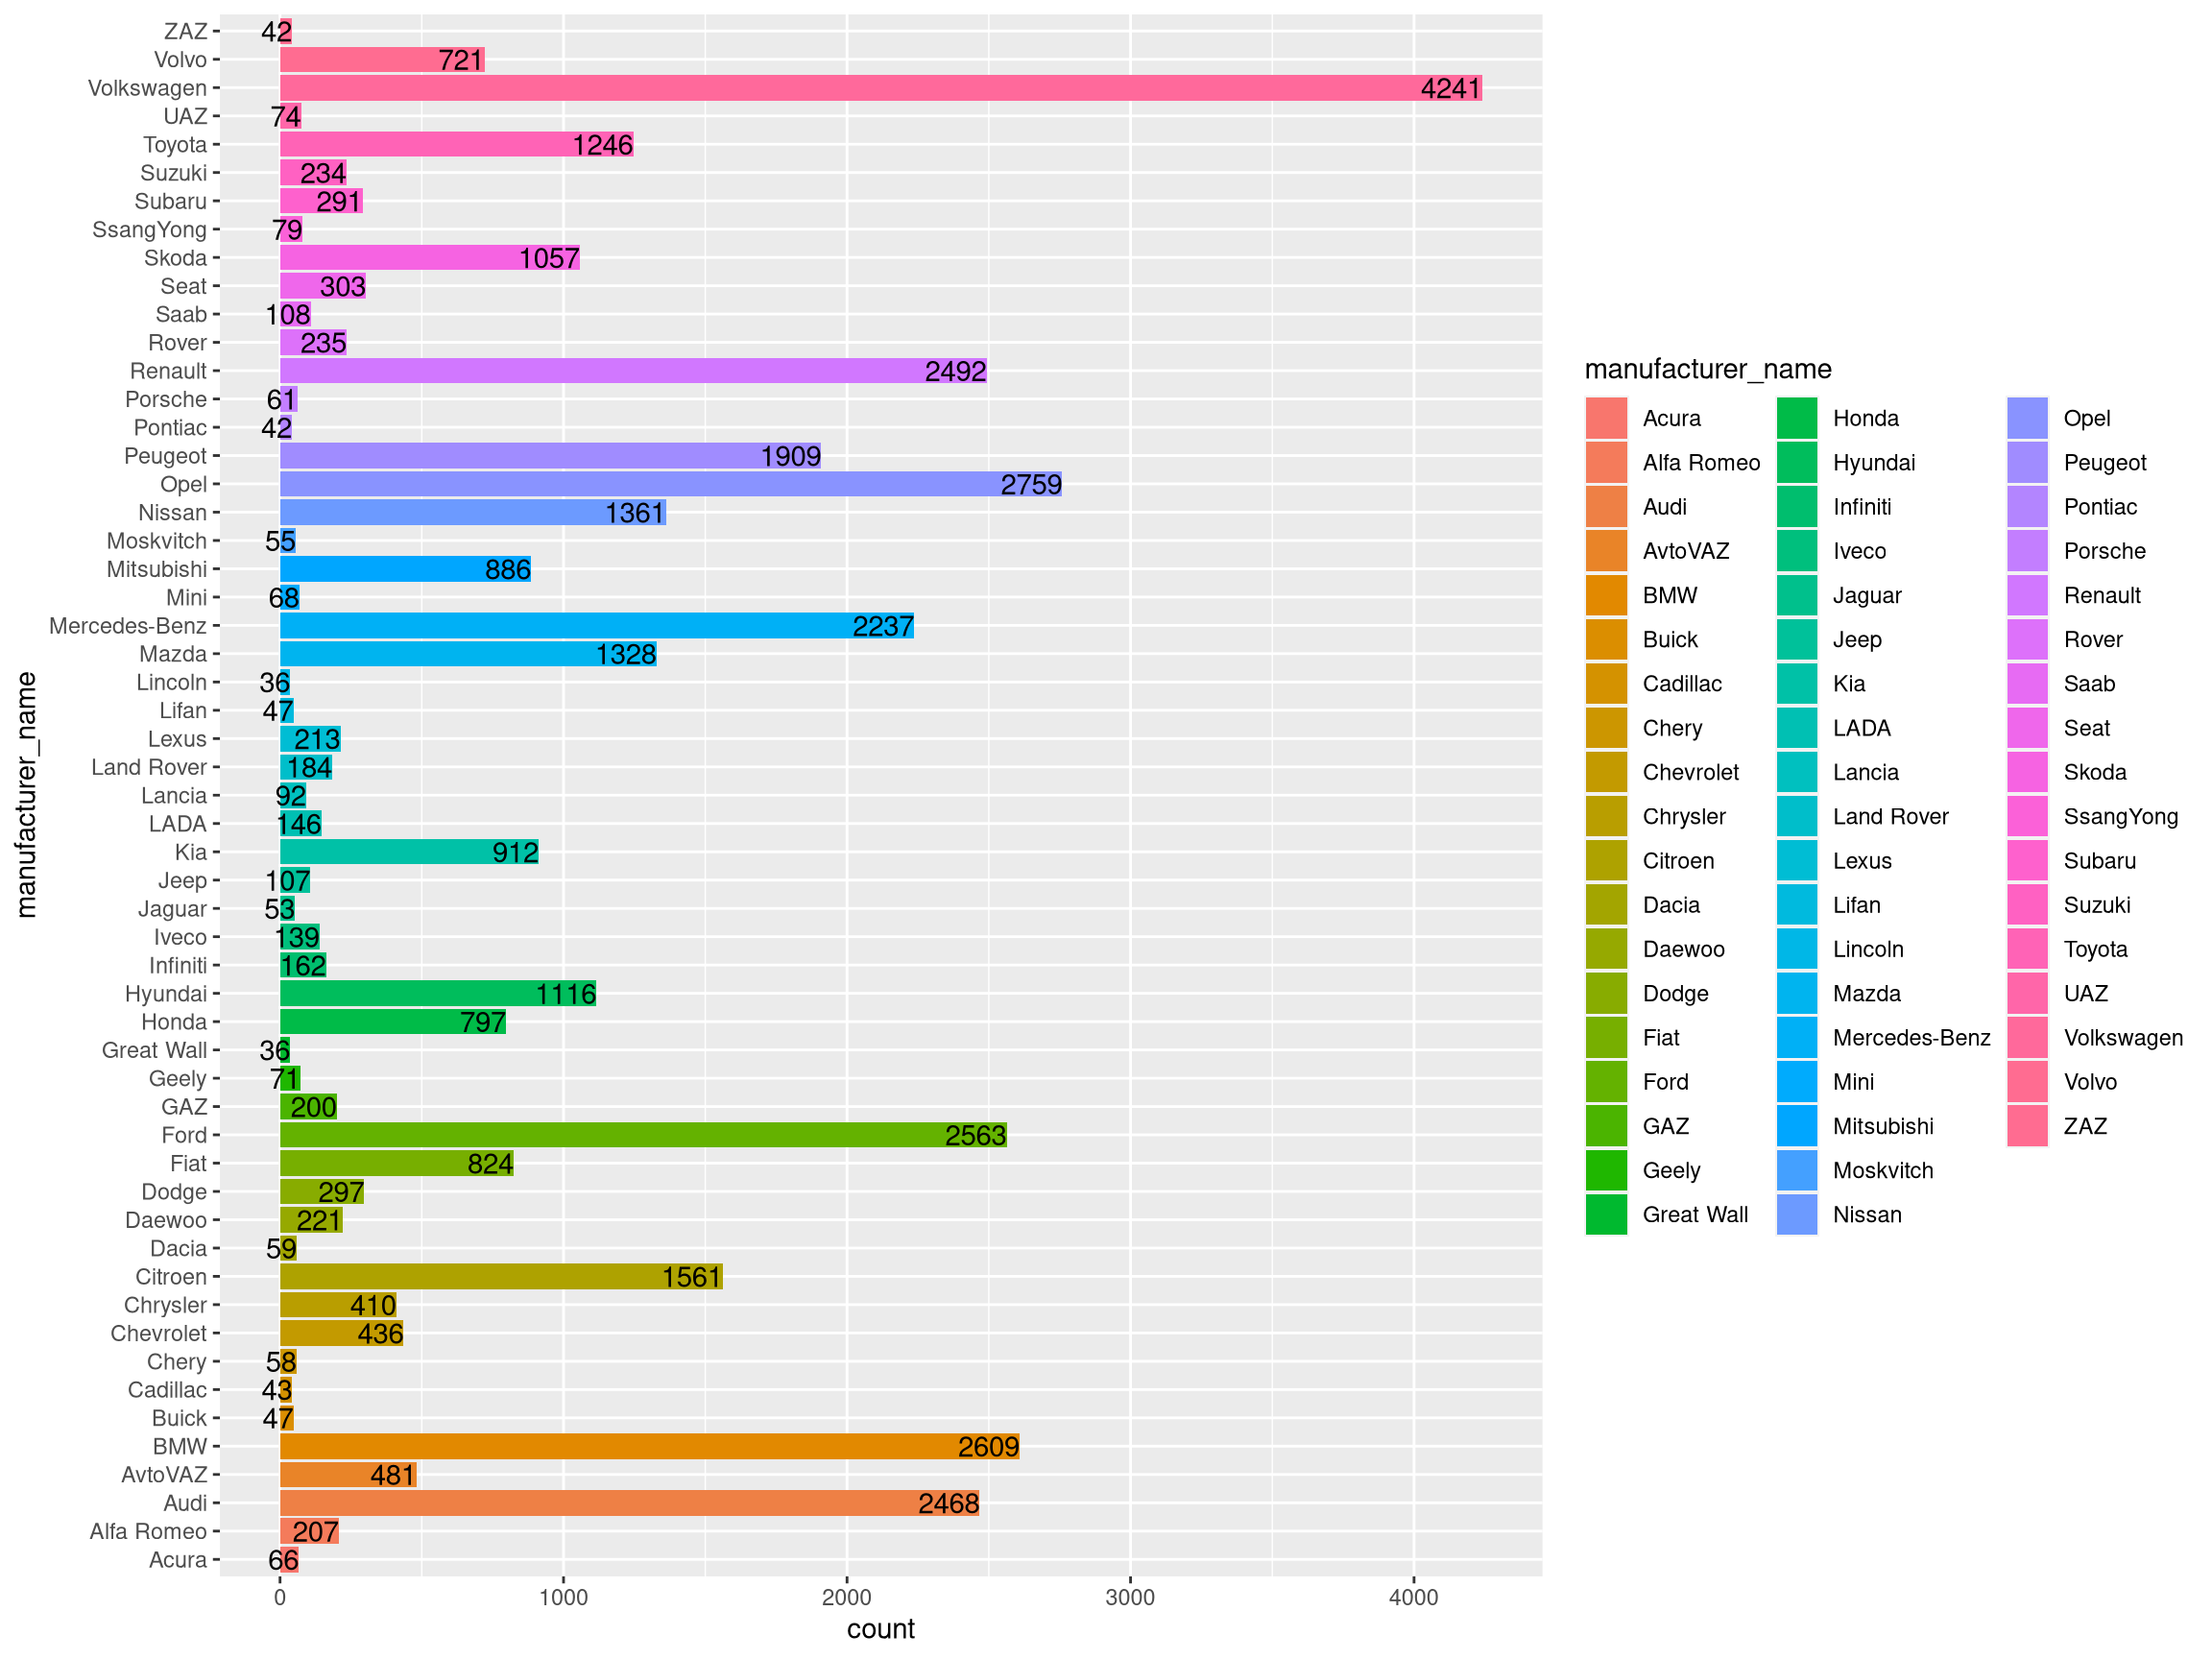
\includegraphics{Group1Report_files/figure-latex/manufacturerVsCount-1.pdf}

Once the distribution of the Manufacturers was plotted, we turned our
attention onto the second part of the question: Whether manufacturers
have a significant impact on the asking price of a vehicle?

Another bar graph was used as a means of quickly inspecting how average
price ranged between different manufacturers.

\begin{Shaded}
\begin{Highlighting}[]
\NormalTok{manuPriceDF }\OtherTok{\textless{}{-}} \FunctionTok{group\_by}\NormalTok{(cars\_edited, manufacturer\_name)}
\NormalTok{manuPriceDF\_averages }\OtherTok{\textless{}{-}} \FunctionTok{summarise}\NormalTok{(manuPriceDF, }\AttributeTok{average\_price\_usd =} \FunctionTok{mean}\NormalTok{(price\_usd))}
\FunctionTok{ggplot}\NormalTok{(manuPriceDF\_averages, }\FunctionTok{aes}\NormalTok{(}\AttributeTok{x =}\NormalTok{ average\_price\_usd, }\AttributeTok{y =}\NormalTok{ manufacturer\_name)) }\SpecialCharTok{+} \FunctionTok{geom\_bar}\NormalTok{(}\FunctionTok{aes}\NormalTok{(}\AttributeTok{fill =}\NormalTok{ manufacturer\_name),}\AttributeTok{stat=}\StringTok{"identity"}\NormalTok{) }\SpecialCharTok{+} \FunctionTok{geom\_text}\NormalTok{(}\FunctionTok{aes}\NormalTok{(}\AttributeTok{label =}  \FunctionTok{paste0}\NormalTok{(}\StringTok{"$"}\NormalTok{,}\FunctionTok{round}\NormalTok{(average\_price\_usd)), }\AttributeTok{hjust =} \DecValTok{1}\NormalTok{))}
\end{Highlighting}
\end{Shaded}

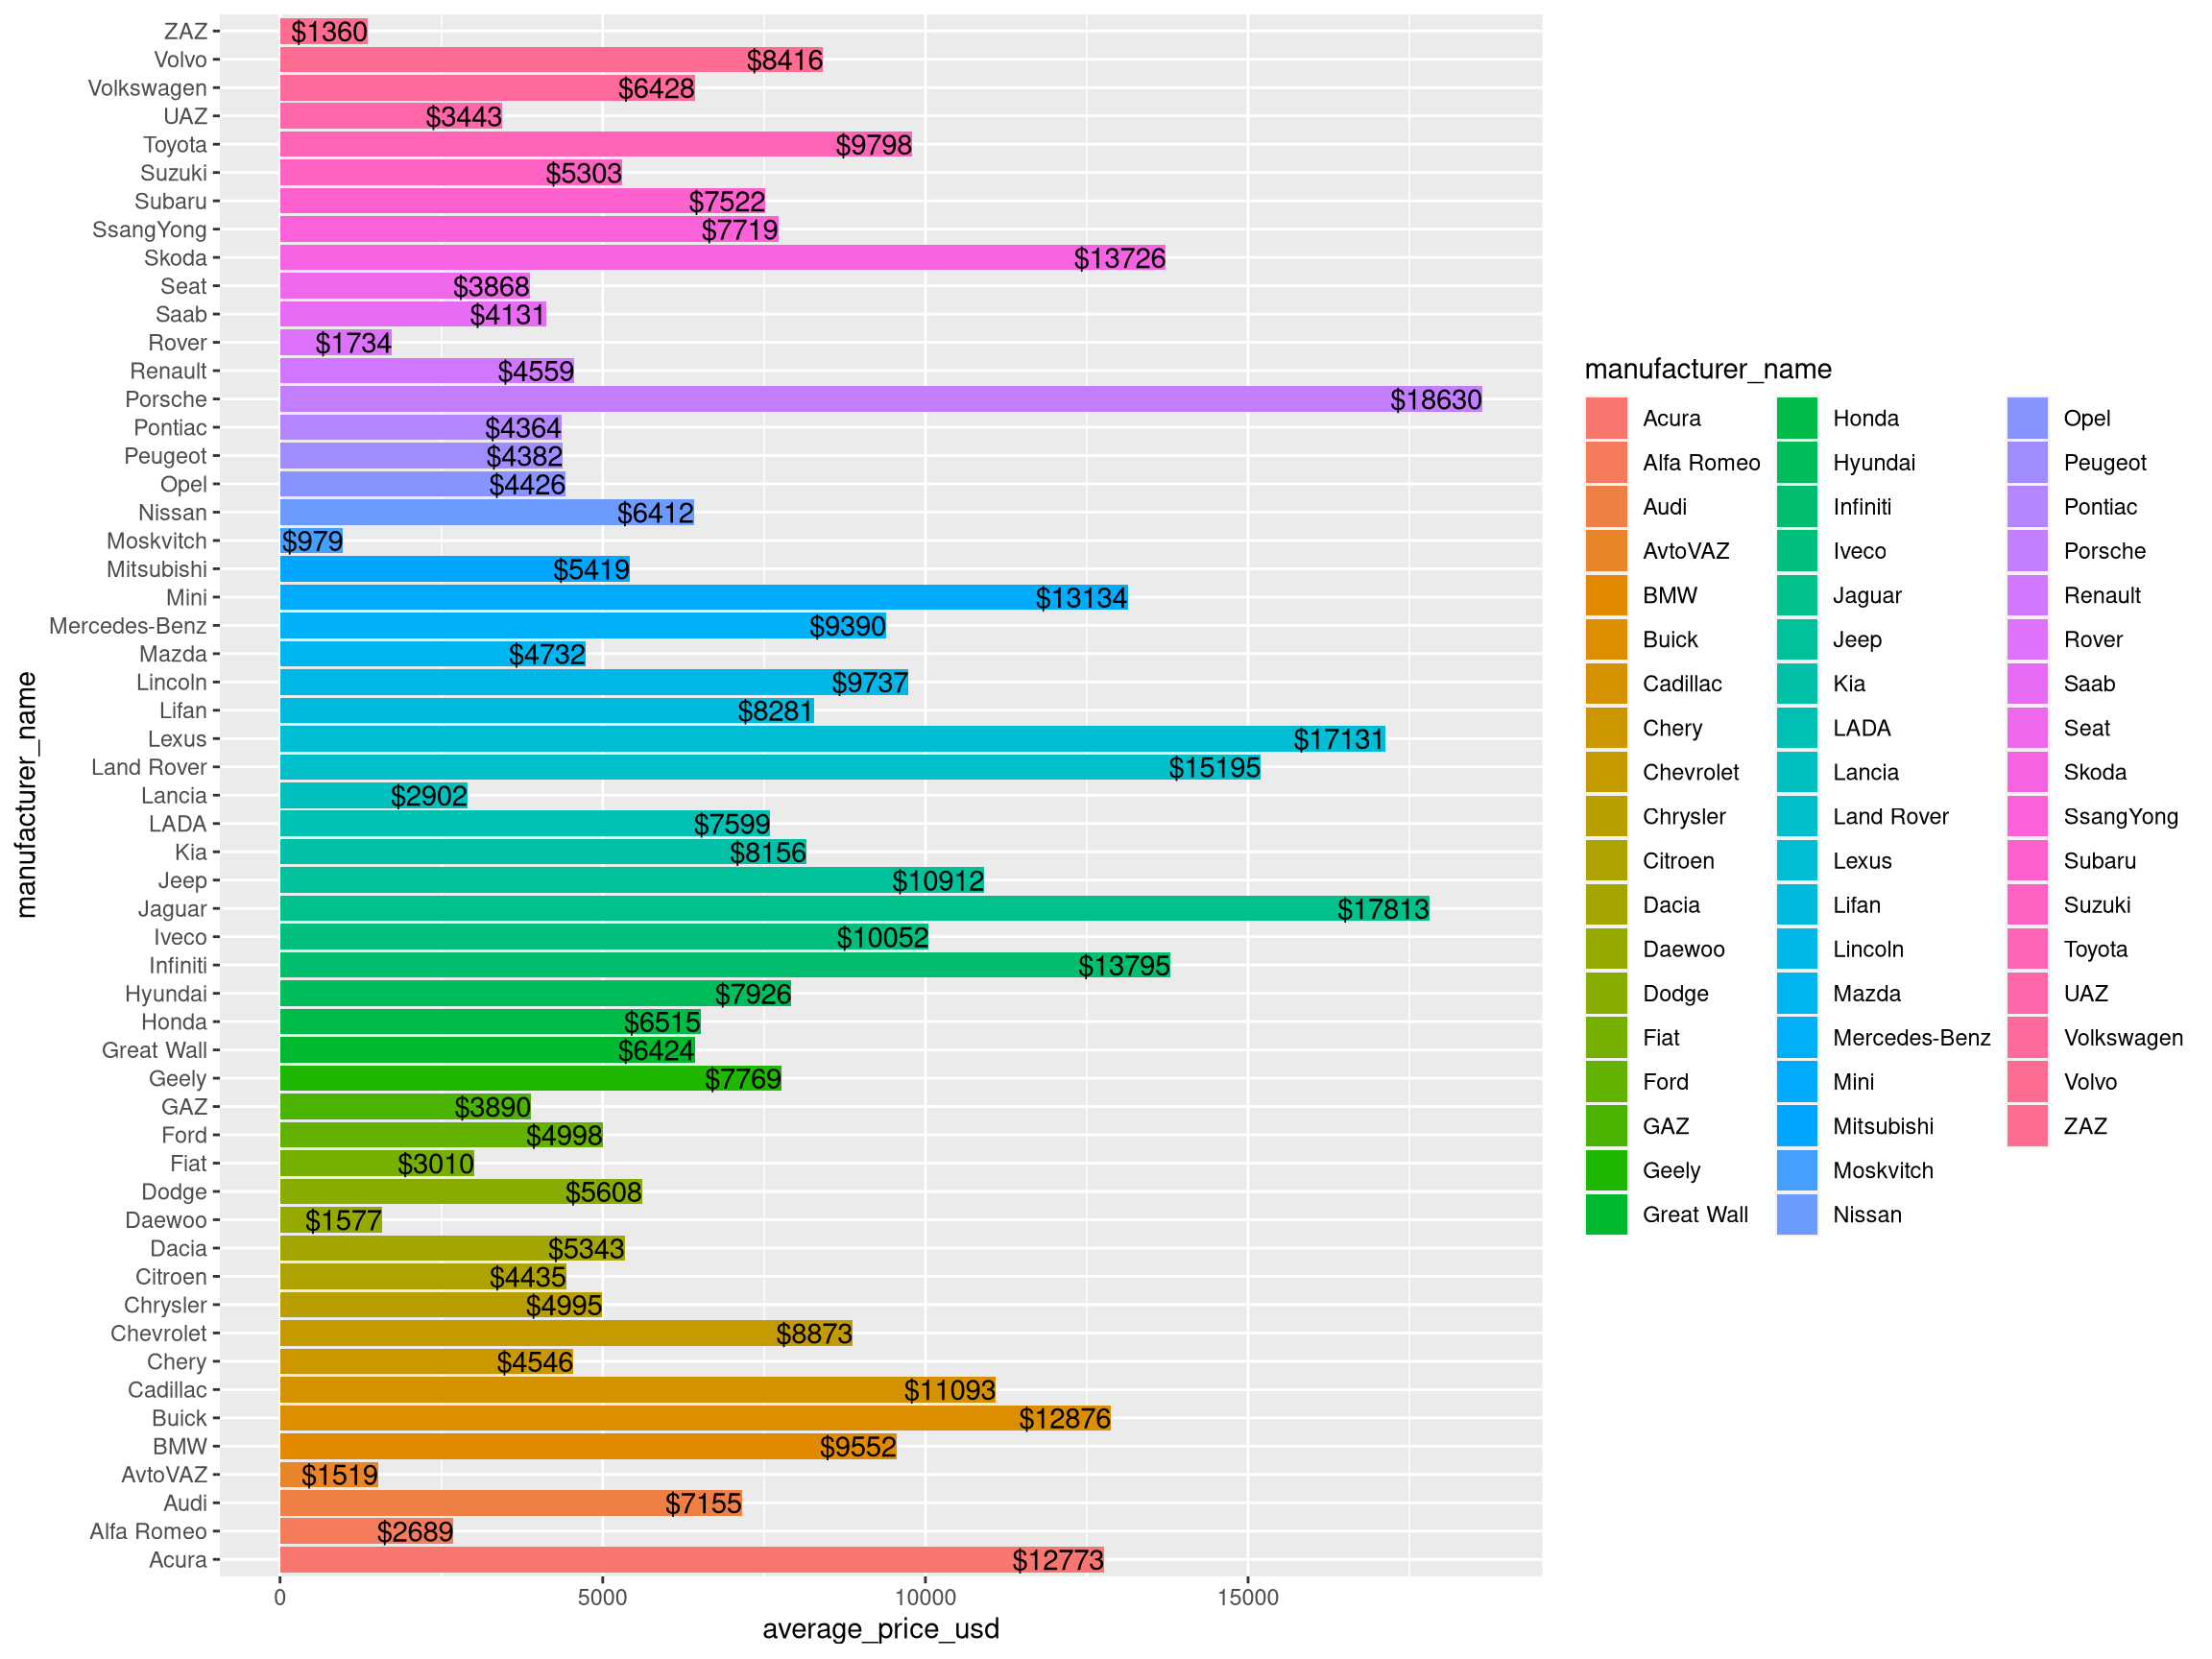
\includegraphics{Group1Report_files/figure-latex/manufacturerVsPrice-1.pdf}

Looking at the bar graph we can predict that the manufacturer of a
vehicle has an impact on asking price. Nevertheless, observation is not
sufficient evidence and so we proceed by testing this claim. Once again,
we are dealing with categorical data and we wish to compare the means of
the prices for the Manufacturers. Naturally, we chose the One-Way Anova
test to test our claim.

The hypotheses for the test are as follows:

H\textsubscript{0} = The mean prices of the different groups are the
same

H\textsubscript{a} = At least one sample mean price is not equal to the
others

Furthermore, we will use 0.05 as our significance level. The result of
the Anova test was the following:

\begin{Shaded}
\begin{Highlighting}[]
\NormalTok{manuSumm }\OtherTok{\textless{}{-}} \FunctionTok{group\_by}\NormalTok{(manuPriceDF, manuPriceDF}\SpecialCharTok{$}\NormalTok{manufacturer\_name) }\SpecialCharTok{\%\textgreater{}\%}
  \FunctionTok{summarise}\NormalTok{(}
    \AttributeTok{count =} \FunctionTok{n}\NormalTok{(),}
    \AttributeTok{mean =} \FunctionTok{mean}\NormalTok{(price\_usd, }\AttributeTok{na.rm =} \ConstantTok{TRUE}\NormalTok{),}
    \AttributeTok{sd =} \FunctionTok{sd}\NormalTok{(price\_usd, }\AttributeTok{na.rm =} \ConstantTok{TRUE}\NormalTok{)}
\NormalTok{  )}

\CommentTok{\# Compute the analysis of variance}
\NormalTok{res.aovTwo }\OtherTok{\textless{}{-}} \FunctionTok{aov}\NormalTok{(manuPriceDF}\SpecialCharTok{$}\NormalTok{price\_usd }\SpecialCharTok{\textasciitilde{}}\NormalTok{ manuPriceDF}\SpecialCharTok{$}\NormalTok{manufacturer\_name,}
                  \AttributeTok{data =}\NormalTok{ manuPriceDF)}

\FunctionTok{summary}\NormalTok{(res.aovTwo)}
\end{Highlighting}
\end{Shaded}

\begin{verbatim}
##                                  Df    Sum Sq   Mean Sq F value Pr(>F)    
## manuPriceDF$manufacturer_name    54 2.917e+11 5.402e+09   160.1 <2e-16 ***
## Residuals                     38435 1.297e+12 3.374e+07                   
## ---
## Signif. codes:  0 '***' 0.001 '**' 0.01 '*' 0.05 '.' 0.1 ' ' 1
\end{verbatim}

Investigating the results of the one-way Anova we can confirm our claim.
The p-value was less than 0.05(\textless2e-16) and so we conclude that
there are significant differences between the manufacturers.

We continue with the Tukey HSD to do multiple pairwise-comparisons
between the means of our groups. This will allow us to see exactly which
manufacturers significantly differ in asking price.

\begin{Shaded}
\begin{Highlighting}[]
\CommentTok{\# Result omitted for brevity\textquotesingle{}s sake}
\CommentTok{\# Tukey Test}
\FunctionTok{TukeyHSD}\NormalTok{(res.aovTwo)}
\end{Highlighting}
\end{Shaded}

With the results see that numerous manufacturers are statistically
different, and we can use this data to list every statistically
different manufacturer.

\textbf{We can confirm that there is a relationship between the
manufacturer and asking price.}

\begin{center}\rule{0.5\linewidth}{0.5pt}\end{center}

\hypertarget{q3-what-is-the-relationship-between-odometer-and-price}{%
\paragraph{\texorpdfstring{\textbf{Q3:} What is the relationship between
odometer and
price?}{Q3: What is the relationship between odometer and price?}}\label{q3-what-is-the-relationship-between-odometer-and-price}}

\textbf{A: There is a low negative correlation between price and
odometer.}

\textbf{Justification:}

Initially a Scatter plot was used to quickly inspect for possible
relationships between price and odometer.

\begin{verbatim}
## `geom_smooth()` using method = 'gam' and formula 'y ~ s(x, bs = "cs")'
\end{verbatim}

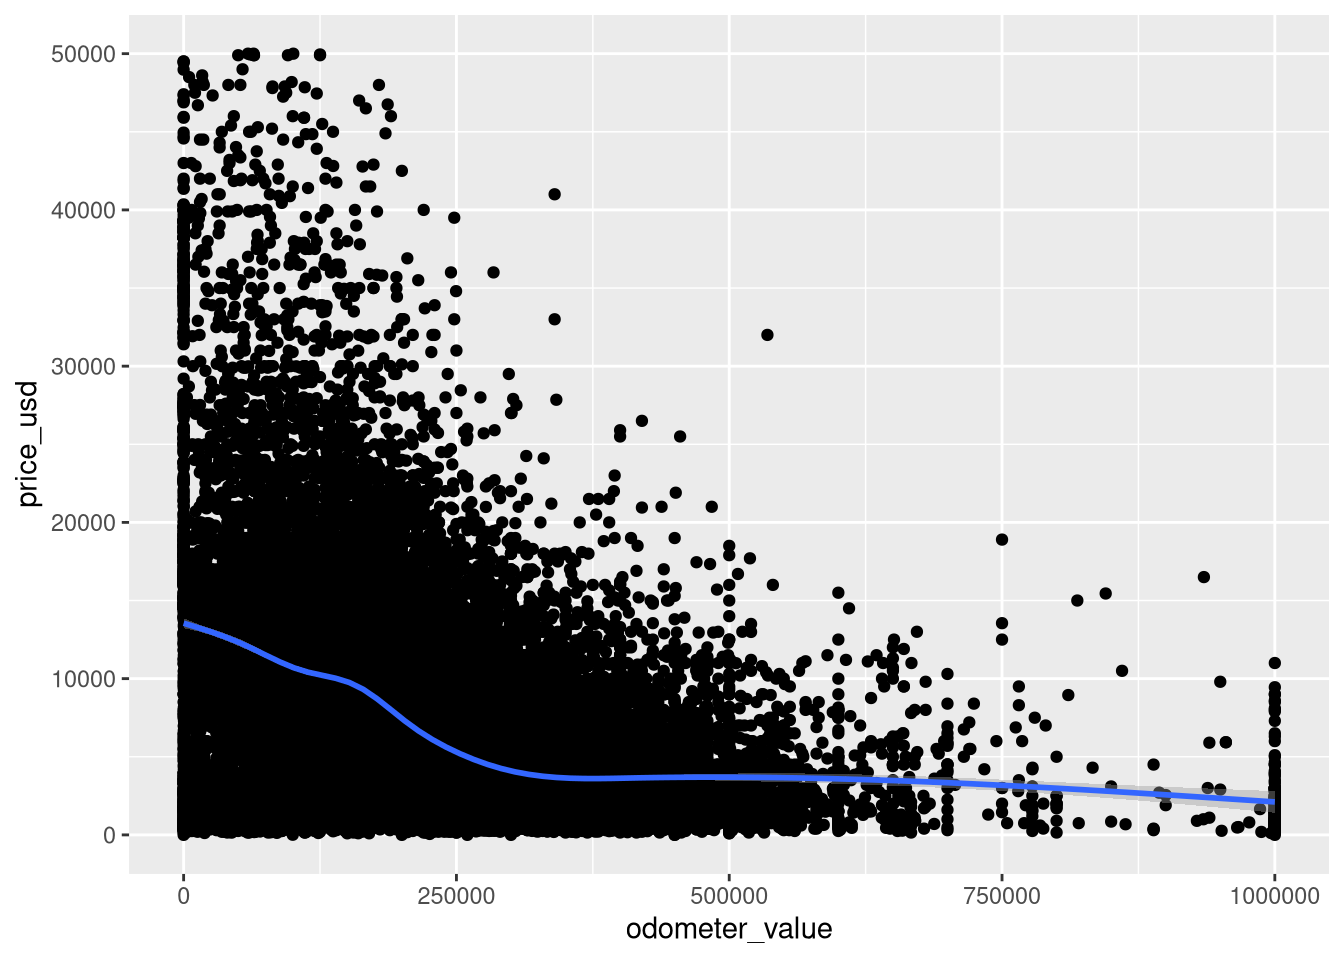
\includegraphics{Group1Report_files/figure-latex/OdometerPrice-1.pdf}

When we investigate this graph, we initially notice that the line of
best fit seems to be going down as the odometer value increases.
Nevertheless, the data had a significant amount of variation and further
testing would need to be done to confirm our results.

Since we are investigating the relationship between 2 continuous
variables, we begin by using a correlation test.

The hypotheses for the test are as follows:

H\textsubscript{0} =There does not exist a correlation between Odometer
Value and Vehicle Price

H\textsubscript{a} = There does exist a correlation between Odometer
Value and Vehicle Price

Furthermore, we will use 0.05 as our significance level. The result of
the correlation test was the following:

\begin{Shaded}
\begin{Highlighting}[]
\CommentTok{\#Getting cor value}
\FunctionTok{cor.test}\NormalTok{(cars\_edited}\SpecialCharTok{$}\NormalTok{odometer\_value, cars\_edited}\SpecialCharTok{$}\NormalTok{price\_usd)}
\end{Highlighting}
\end{Shaded}

\begin{verbatim}
## 
##  Pearson's product-moment correlation
## 
## data:  cars_edited$odometer_value and cars_edited$price_usd
## t = -90.821, df = 38488, p-value < 2.2e-16
## alternative hypothesis: true correlation is not equal to 0
## 95 percent confidence interval:
##  -0.4282966 -0.4118421
## sample estimates:
##        cor 
## -0.4201039
\end{verbatim}

Since the p-value is less than 0.05 we can conclude that Price and
Odometer are significantly correlated with a correlation coefficient of
-0.4201039 and p-value of \textless{} 2.2e-16

We continue with our question by investigating how good of an indicator
of price odometer is. To do this we will use linear regression and check
the percentage of accuracy of that line. Afterwards, we will graph the
linear regression line to provide us with a useful visual.

\begin{Shaded}
\begin{Highlighting}[]
\FunctionTok{set.seed}\NormalTok{(}\DecValTok{123}\NormalTok{)}
\NormalTok{odometer\_on\_price }\OtherTok{\textless{}{-}} \FunctionTok{lm}\NormalTok{ (price\_usd }\SpecialCharTok{\textasciitilde{}}\NormalTok{ odometer\_value, }\AttributeTok{data =}\NormalTok{ cars\_edited)}

\FunctionTok{ggplot}\NormalTok{ (cars\_edited, }\FunctionTok{aes}\NormalTok{(}\AttributeTok{x=}\NormalTok{odometer\_value, }\AttributeTok{y=}\NormalTok{price\_usd)) }\SpecialCharTok{+} \FunctionTok{geom\_point}\NormalTok{() }\SpecialCharTok{+} \FunctionTok{stat\_smooth}\NormalTok{(}\AttributeTok{method=}\NormalTok{lm)}
\end{Highlighting}
\end{Shaded}

\begin{verbatim}
## `geom_smooth()` using formula 'y ~ x'
\end{verbatim}

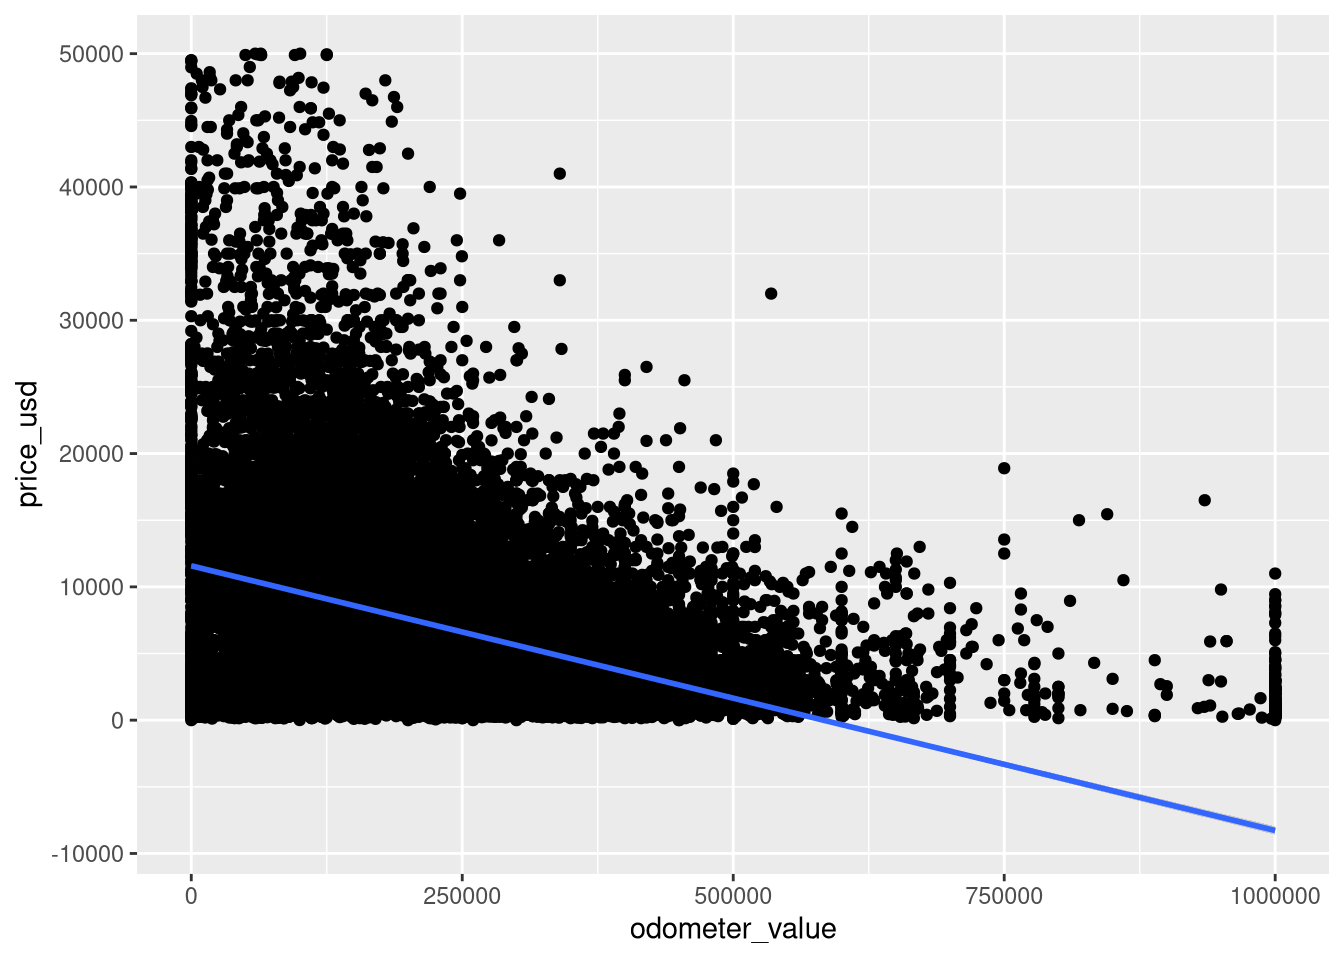
\includegraphics{Group1Report_files/figure-latex/odometerLm-1.pdf}

Once the linear regression model is created and graphed, we proceed to
check the R2 to see the proportion of the prices that can be explained
by the model, the variability of the beta coefficients, and the
percentage error.

\begin{Shaded}
\begin{Highlighting}[]
\FunctionTok{summary}\NormalTok{(odometer\_on\_price)}
\end{Highlighting}
\end{Shaded}

\begin{verbatim}
## 
## Call:
## lm(formula = price_usd ~ odometer_value, data = cars_edited)
## 
## Residuals:
##    Min     1Q Median     3Q    Max 
## -11577  -3514  -1122   2064  40854 
## 
## Coefficients:
##                  Estimate Std. Error t value Pr(>|t|)    
## (Intercept)     1.158e+04  6.203e+01  186.65   <2e-16 ***
## odometer_value -1.986e-02  2.186e-04  -90.82   <2e-16 ***
## ---
## Signif. codes:  0 '***' 0.001 '**' 0.01 '*' 0.05 '.' 0.1 ' ' 1
## 
## Residual standard error: 5830 on 38488 degrees of freedom
## Multiple R-squared:  0.1765, Adjusted R-squared:  0.1765 
## F-statistic:  8248 on 1 and 38488 DF,  p-value: < 2.2e-16
\end{verbatim}

\begin{Shaded}
\begin{Highlighting}[]
\FunctionTok{confint}\NormalTok{(odometer\_on\_price)}
\end{Highlighting}
\end{Shaded}

\begin{verbatim}
##                        2.5 %        97.5 %
## (Intercept)     1.145654e+04  1.169971e+04
## odometer_value -2.028451e-02 -1.942748e-02
\end{verbatim}

\begin{Shaded}
\begin{Highlighting}[]
\CommentTok{\#                       2.5 \%        97.5 \%}
\CommentTok{\#(Intercept)     1.147053e+04  1.171322e+04}
\CommentTok{\#odometer\_value {-}2.032581e{-}02 {-}1.947015e{-}02}

\FunctionTok{sigma}\NormalTok{(odometer\_on\_price)}\SpecialCharTok{*}\DecValTok{100}\SpecialCharTok{/}\FunctionTok{mean}\NormalTok{(cars\_edited}\SpecialCharTok{$}\NormalTok{price\_usd)}
\end{Highlighting}
\end{Shaded}

\begin{verbatim}
## [1] 87.89188
\end{verbatim}

\begin{Shaded}
\begin{Highlighting}[]
\CommentTok{\# [1] 87.80444}
\end{Highlighting}
\end{Shaded}

The R2 is 0.1774 which indicates that a low proportion of prices in the
data can be explained by the model. Furthermore, the percentage error is
87.80444 which confirms how poor an exploratory model would be if it
solely used odometer to predict price.

\textbf{We can conclude that the higher the odometer the lower the price
of the vehicle will be.} Nevertheless, our linear regression model
informs us that to create an accurate model we will need to consider
more attributes.

\begin{center}\rule{0.5\linewidth}{0.5pt}\end{center}

\hypertarget{q4-does-the-number-of-photos-a-vehicle-has-impact-the-selling-price}{%
\paragraph{\texorpdfstring{\textbf{Q4:} Does the number of photos a
vehicle has impact the selling
price?}{Q4: Does the number of photos a vehicle has impact the selling price?}}\label{q4-does-the-number-of-photos-a-vehicle-has-impact-the-selling-price}}

\textbf{A: There exists a low positive correlation between number of
photos a vehicle has and the selling price.}

\textbf{Justification:}

To gain an intuitive understanding of the question we sought to use a
scatter plot to see the relationship between price and number of photos.

\begin{Shaded}
\begin{Highlighting}[]
\CommentTok{\#Scatter plot: Number of photos and price}
\FunctionTok{ggplot}\NormalTok{(cars\_edited, }\FunctionTok{aes}\NormalTok{( }\AttributeTok{x =}\NormalTok{number\_of\_photos, }\AttributeTok{y=}\NormalTok{price\_usd)) }\SpecialCharTok{+} \FunctionTok{geom\_hex}\NormalTok{() }\SpecialCharTok{+} \FunctionTok{stat\_smooth}\NormalTok{(}\AttributeTok{color =} \StringTok{"red"}\NormalTok{) }
\end{Highlighting}
\end{Shaded}

\begin{verbatim}
## `geom_smooth()` using method = 'gam' and formula 'y ~ s(x, bs = "cs")'
\end{verbatim}

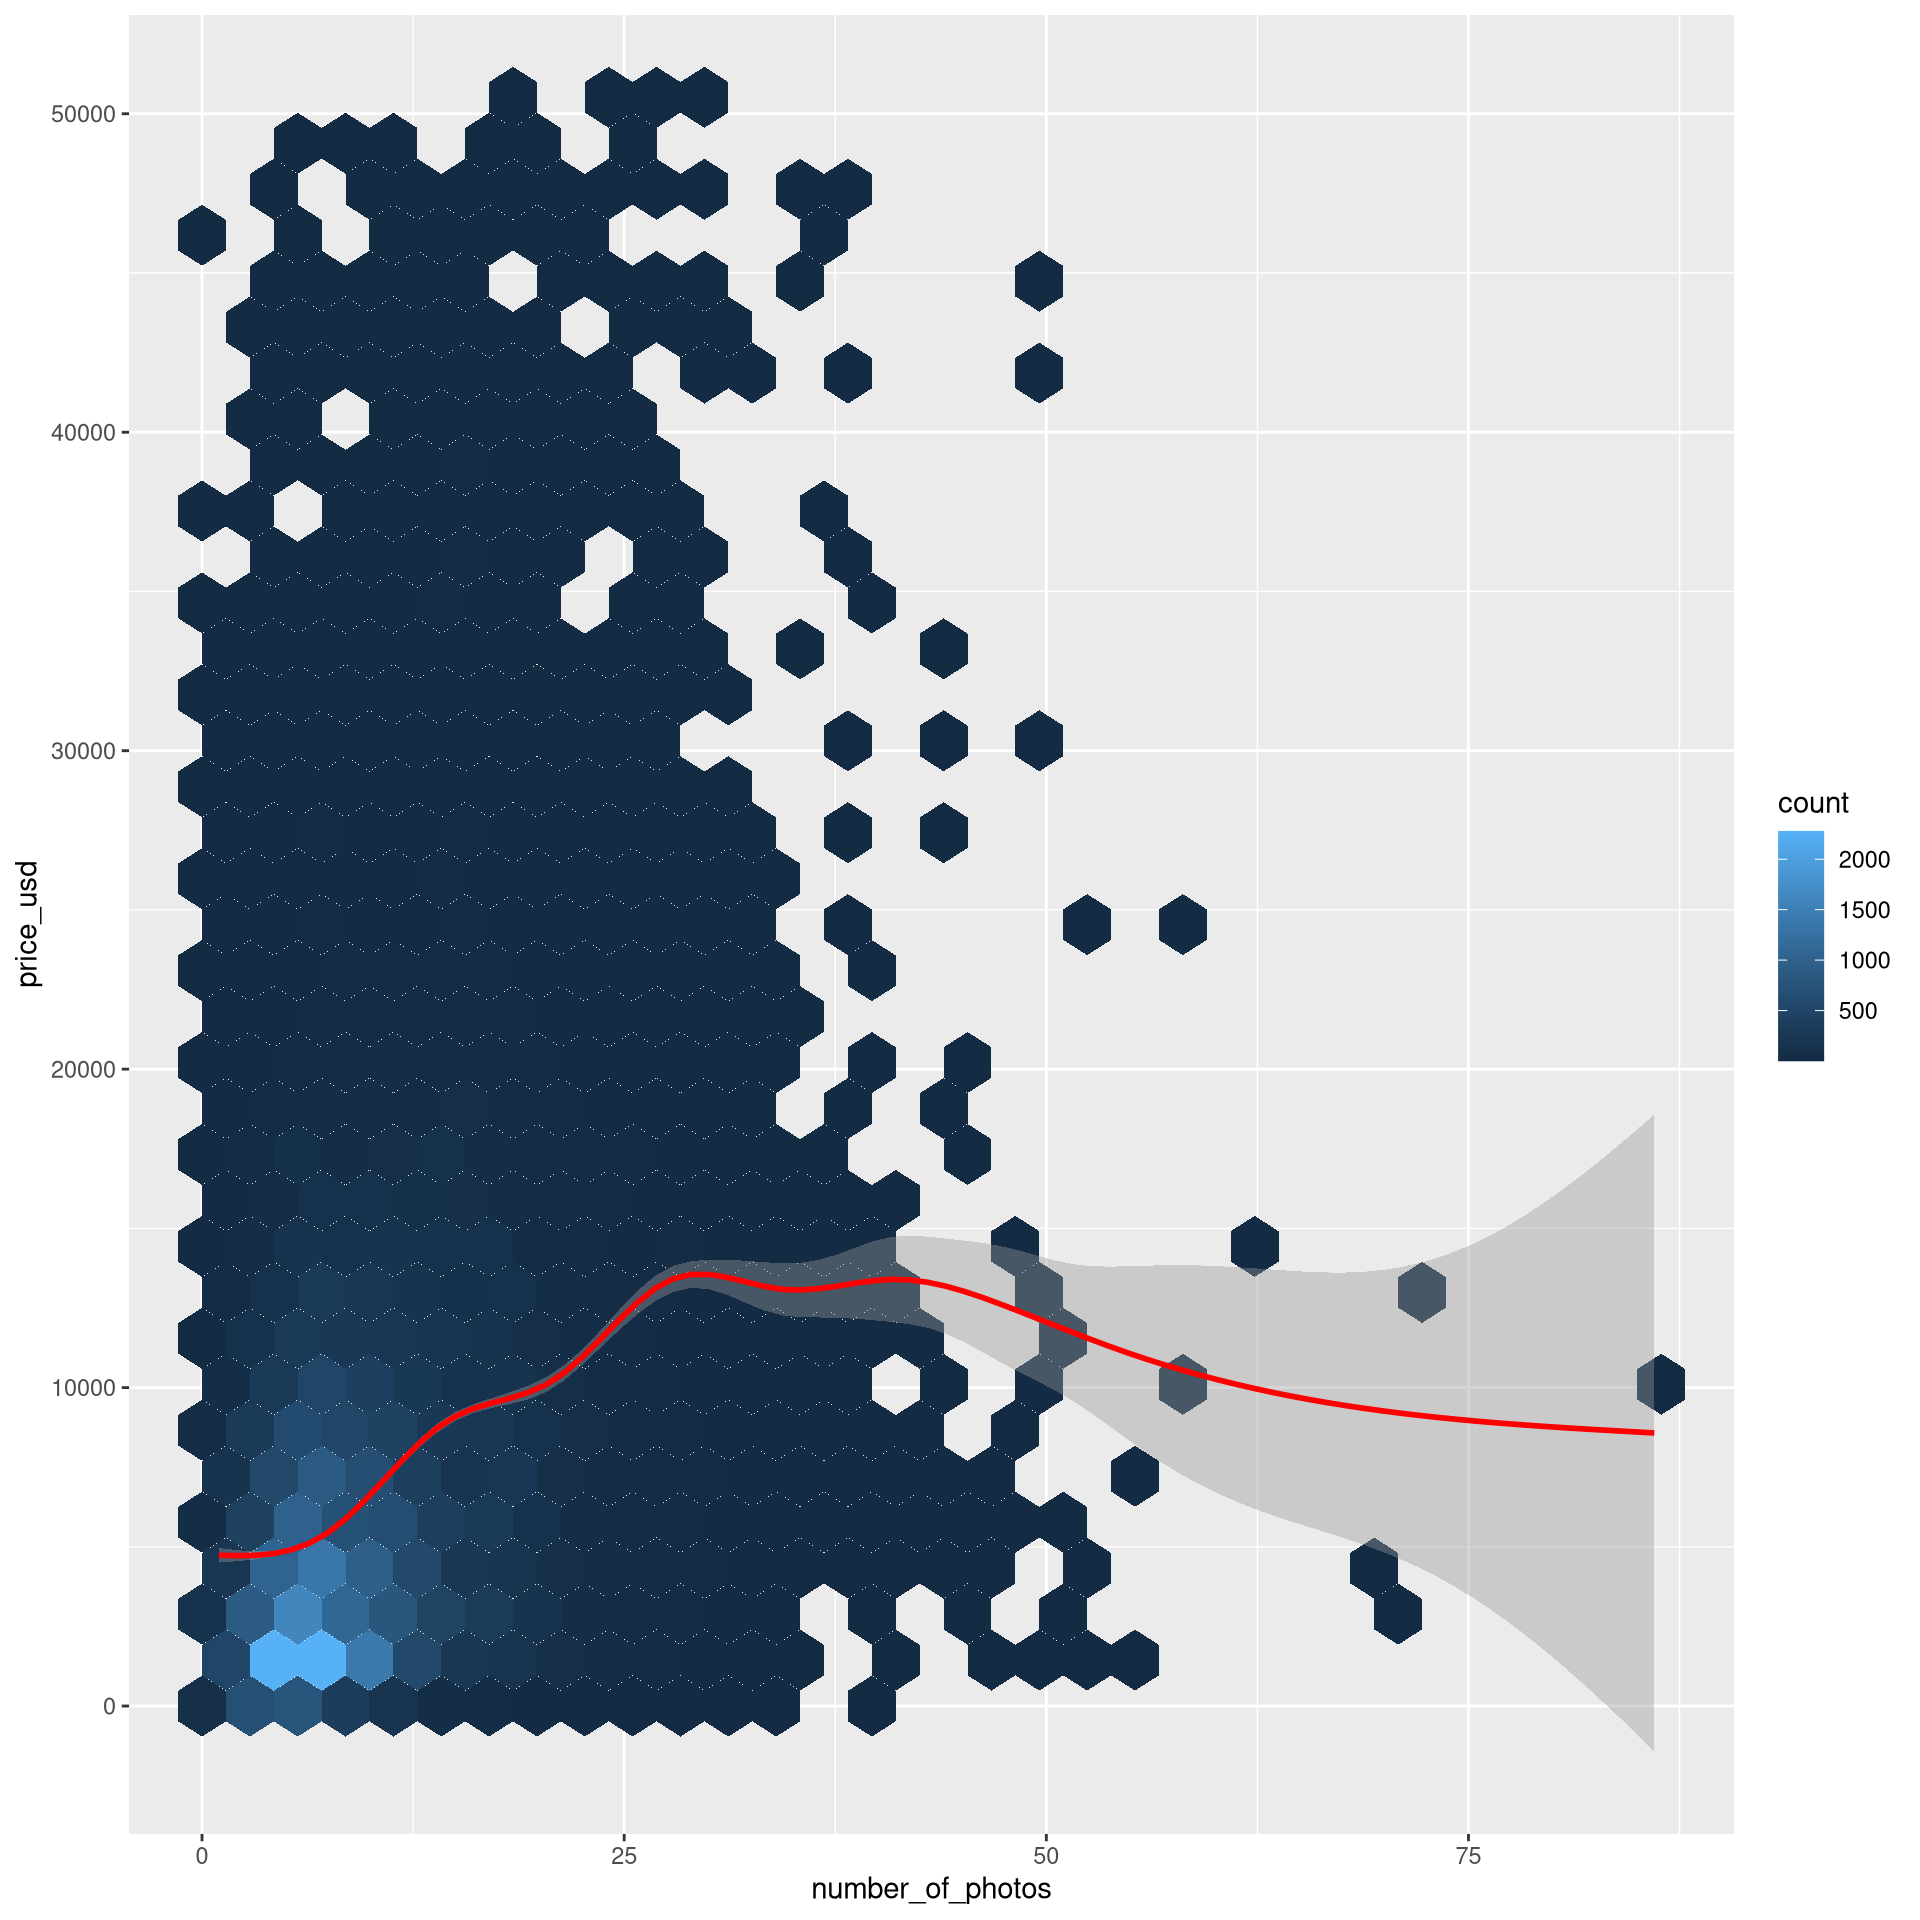
\includegraphics{Group1Report_files/figure-latex/NumPhotosPrice-1.pdf}

When we look at this graph, we can see that although there exists a
line. Nevertheless, the data had a significant amount of variation and
further testing would need to be done to get a result. It does seem that
there will be a very little (if any) correlation between price and
number of photos.

Since we are investigating the relationship between 2 continuous
variables, we will be using the correlation test.

The hypotheses are as follows:

H\textsubscript{0} =There does not exist a correlation between Number of
Photos and Vehicle Price

H\textsubscript{a} = There does exist a correlation between Number of
Photos and Vehicle Price

We will use 0.05 as our significance level. The result of the
correlation test was the following:

\begin{Shaded}
\begin{Highlighting}[]
\CommentTok{\#getting the cor value}
\FunctionTok{cor.test}\NormalTok{(cars\_edited}\SpecialCharTok{$}\NormalTok{number\_of\_photos, cars\_edited}\SpecialCharTok{$}\NormalTok{price\_usd)}
\end{Highlighting}
\end{Shaded}

\begin{verbatim}
## 
##  Pearson's product-moment correlation
## 
## data:  cars_edited$number_of_photos and cars_edited$price_usd
## t = 65.382, df = 38488, p-value < 2.2e-16
## alternative hypothesis: true correlation is not equal to 0
## 95 percent confidence interval:
##  0.3071525 0.3251358
## sample estimates:
##       cor 
## 0.3161726
\end{verbatim}

Since the p-value is less than 0.05 we can conclude that Price and
Number of Photos are significantly correlated with a correlation
coefficient of 0.3161726 and p-value of \textless{} 2.2e-16

Next, we aim to investigate how good of an indicator of price the number
of vehicle photos is. We shall employ linear regression, check the
percentage of accuracy of that line, and graph the linear regression
line to provide us with a useful visual.

\begin{Shaded}
\begin{Highlighting}[]
\CommentTok{\#Getting the formula for linear regression}
\FunctionTok{set.seed}\NormalTok{(}\DecValTok{123}\NormalTok{)}
\NormalTok{number\_of\_photos\_on\_price }\OtherTok{\textless{}{-}} \FunctionTok{lm}\NormalTok{ (price\_usd }\SpecialCharTok{\textasciitilde{}}\NormalTok{ number\_of\_photos, }\AttributeTok{data =}\NormalTok{ cars\_edited)}

\CommentTok{\#Scatter plot: Number of photos and price with linear regression line}
\FunctionTok{ggplot}\NormalTok{ (cars\_edited, }\FunctionTok{aes}\NormalTok{(}\AttributeTok{x=}\NormalTok{number\_of\_photos, }\AttributeTok{y=}\NormalTok{price\_usd)) }\SpecialCharTok{+} \FunctionTok{geom\_point}\NormalTok{() }\SpecialCharTok{+} \FunctionTok{stat\_smooth}\NormalTok{(}\AttributeTok{method=}\NormalTok{lm)}
\end{Highlighting}
\end{Shaded}

\begin{verbatim}
## `geom_smooth()` using formula 'y ~ x'
\end{verbatim}

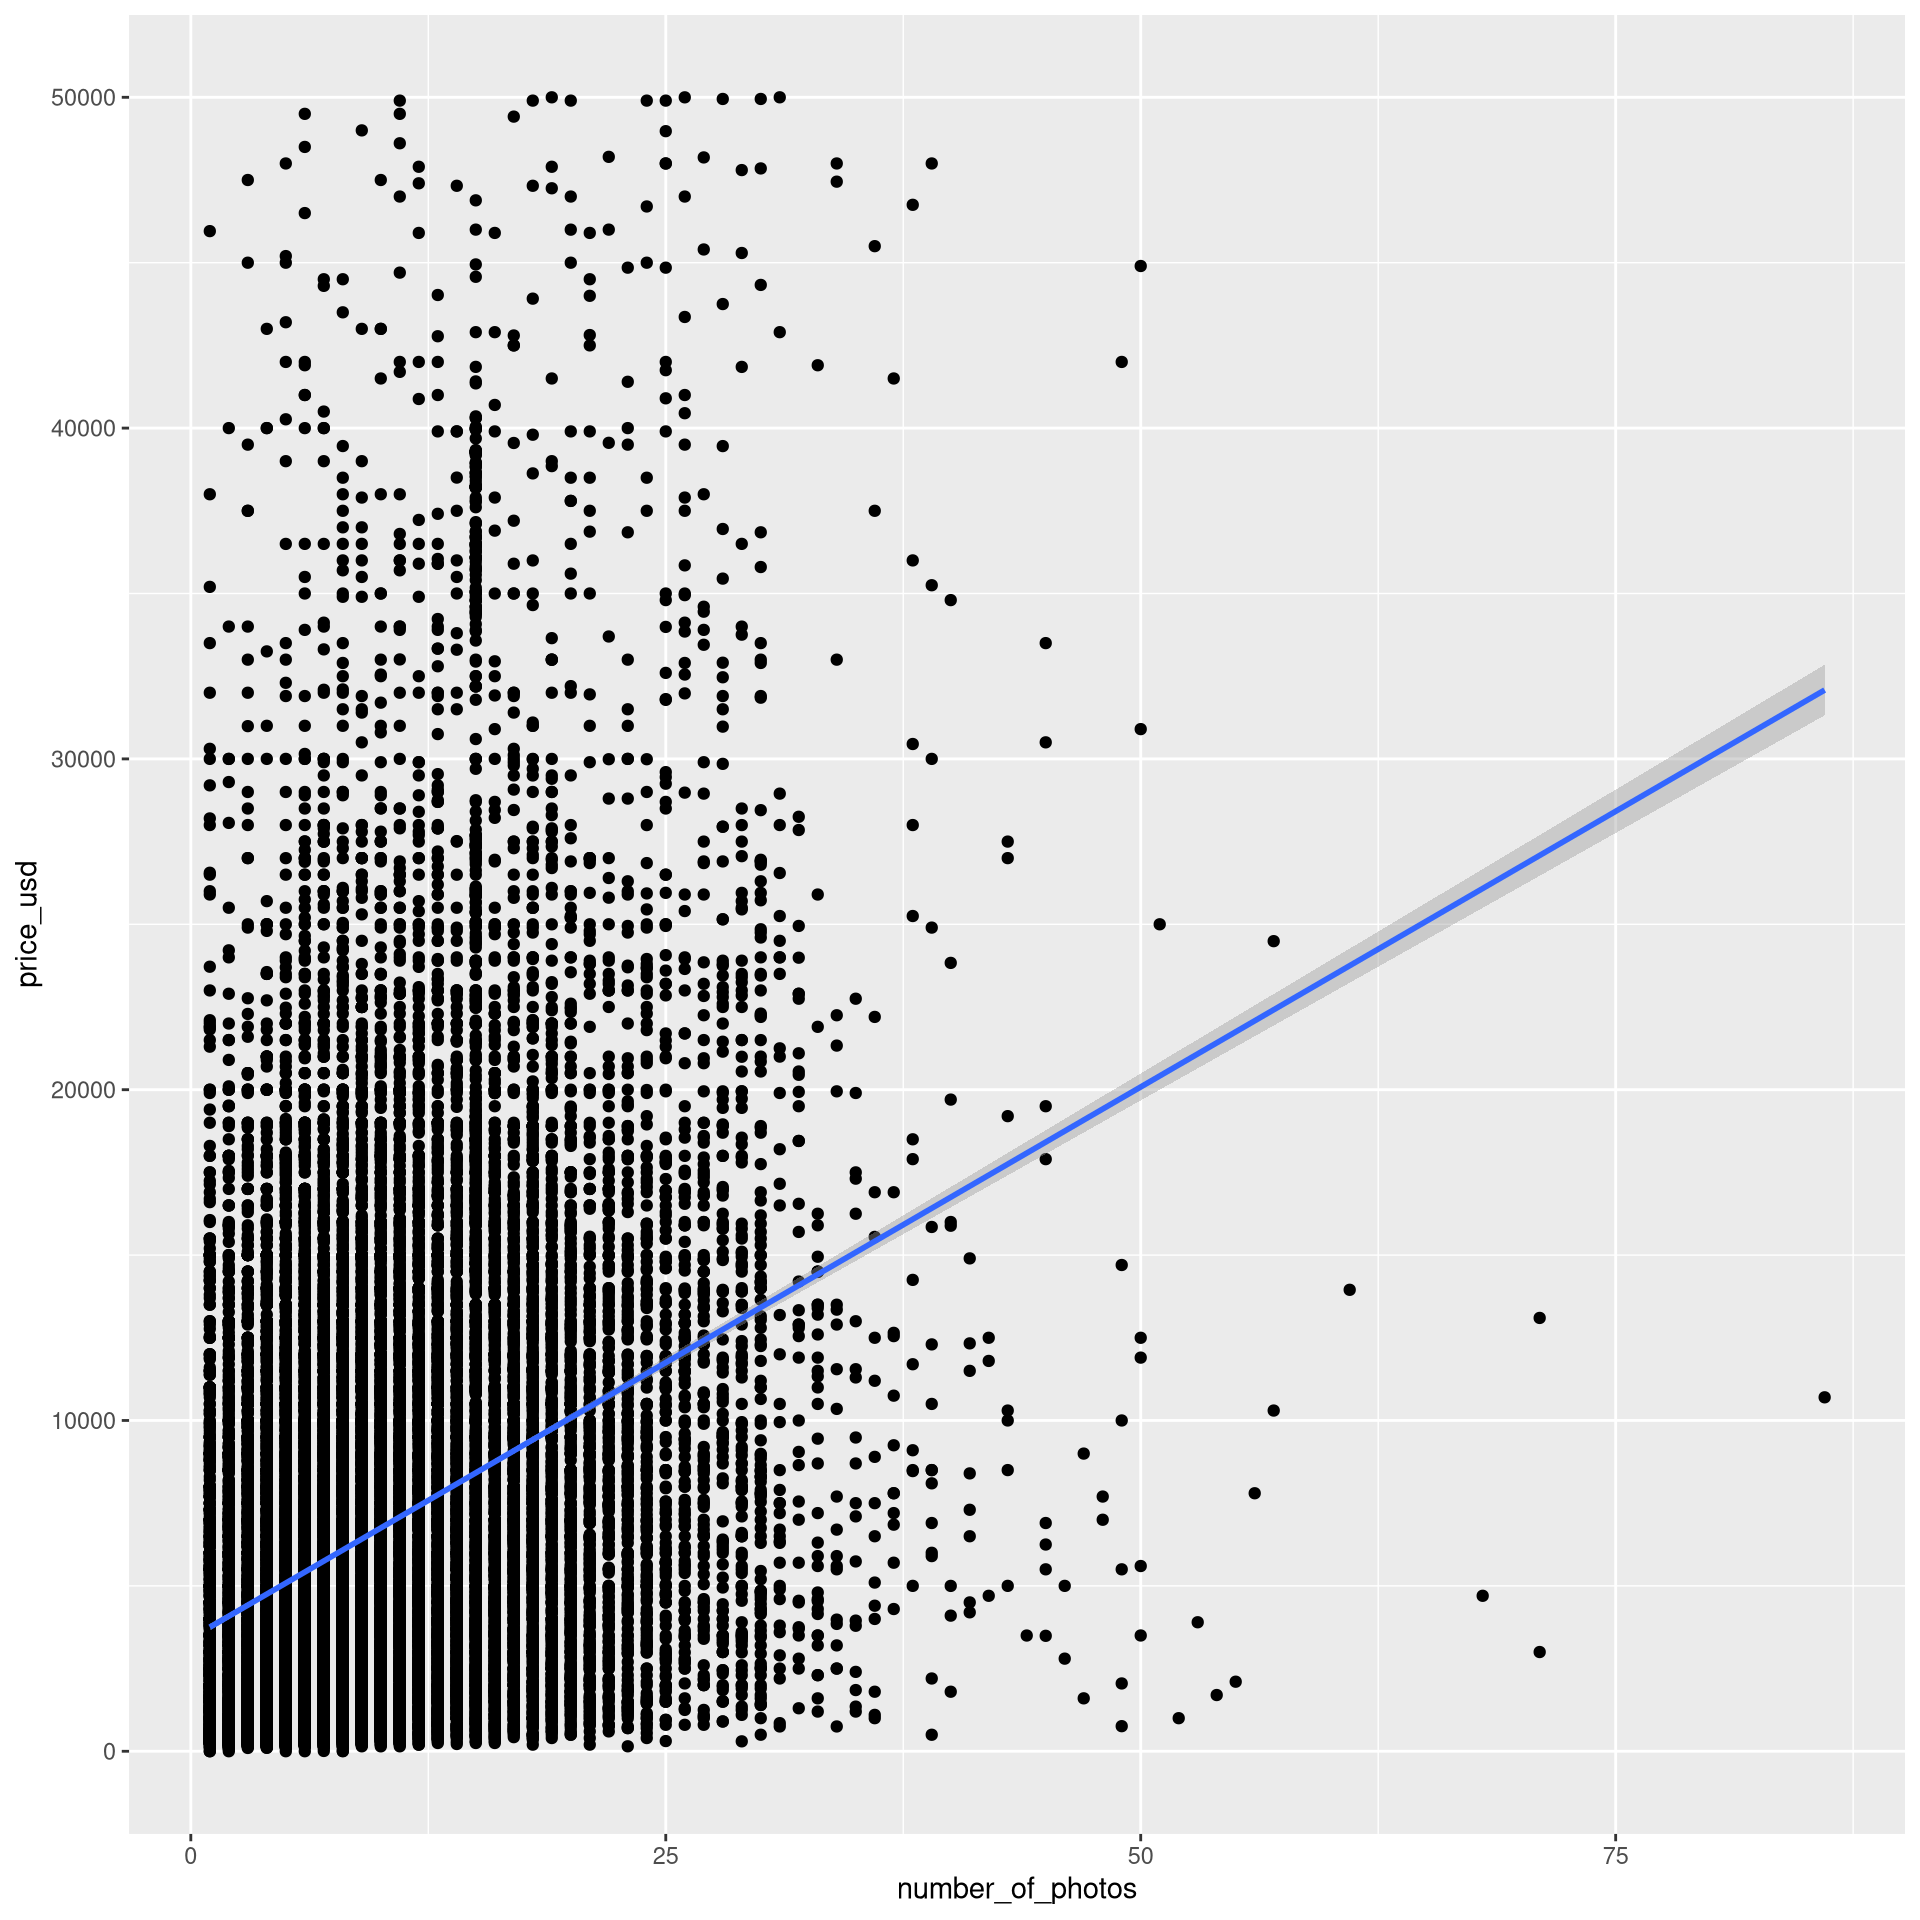
\includegraphics{Group1Report_files/figure-latex/NumPhotosPriceLMandPlot-1.pdf}

Although the linear regression model is created and graphed there
remains information and insights to be gleaned. We proceed to check the
R2 to see the proportion of the prices that can be explained by the
model, the variability of the beta coefficients, and the percentage
error.

\begin{Shaded}
\begin{Highlighting}[]
\FunctionTok{summary}\NormalTok{(number\_of\_photos\_on\_price)}
\end{Highlighting}
\end{Shaded}

\begin{verbatim}
## 
## Call:
## lm(formula = price_usd ~ number_of_photos, data = cars_edited)
## 
## Residuals:
##    Min     1Q Median     3Q    Max 
## -24082  -3884  -1585   2249  44082 
## 
## Coefficients:
##                  Estimate Std. Error t value Pr(>|t|)    
## (Intercept)      3418.275     58.159   58.77   <2e-16 ***
## number_of_photos  333.297      5.098   65.38   <2e-16 ***
## ---
## Signif. codes:  0 '***' 0.001 '**' 0.01 '*' 0.05 '.' 0.1 ' ' 1
## 
## Residual standard error: 6095 on 38488 degrees of freedom
## Multiple R-squared:  0.09997,    Adjusted R-squared:  0.09994 
## F-statistic:  4275 on 1 and 38488 DF,  p-value: < 2.2e-16
\end{verbatim}

\begin{Shaded}
\begin{Highlighting}[]
\CommentTok{\# R\^{}2 is very low(0.1004) which tells us that number of photos is not a good indicator of price. }
\CommentTok{\# We can suspect that several more variables are in play.}

\FunctionTok{confint}\NormalTok{(number\_of\_photos\_on\_price)}
\end{Highlighting}
\end{Shaded}

\begin{verbatim}
##                     2.5 %    97.5 %
## (Intercept)      3304.283 3532.2680
## number_of_photos  323.305  343.2882
\end{verbatim}

\begin{Shaded}
\begin{Highlighting}[]
\CommentTok{\#                     2.5 \%    97.5 \%}
\CommentTok{\#(Intercept)      3300.5010 3528.5452}
\CommentTok{\#number\_of\_photos  324.2843  344.2673}
\FunctionTok{sigma}\NormalTok{(number\_of\_photos\_on\_price)}\SpecialCharTok{*}\DecValTok{100}\SpecialCharTok{/}\FunctionTok{mean}\NormalTok{(cars\_edited}\SpecialCharTok{$}\NormalTok{price\_usd)}
\end{Highlighting}
\end{Shaded}

\begin{verbatim}
## [1] 91.88472
\end{verbatim}

\begin{Shaded}
\begin{Highlighting}[]
\CommentTok{\# Our prediction error rate is extremely high (91.82279\%) which explains the low correlation}
\end{Highlighting}
\end{Shaded}

The R2 is 0.1004 which indicates that a low proportion of prices in the
data can be explained by the model. In other words, number of photos is
not a good indicator of price (more attributes are needed in a model).
Also, the percentage error is 91.82279 which is very high. This confirms
how poor an exploratory model would be if it solely used number of
photos to predict price.

\textbf{We can conclude there is a low negative correlation between
price and odometer.} Our linear regression model tells us that to create
an accurate model we will need to consider more attributes.

\begin{center}\rule{0.5\linewidth}{0.5pt}\end{center}

\hypertarget{q5-does-the-number-of-times-a-vehicle-has-been-upped-in-the-catalog-to-raise-its-position-impact-the-selling-price}{%
\paragraph{\texorpdfstring{\textbf{Q5:} Does the number of times a
vehicle has been upped in the catalog to raise its position impact the
selling
price?}{Q5: Does the number of times a vehicle has been upped in the catalog to raise its position impact the selling price?}}\label{q5-does-the-number-of-times-a-vehicle-has-been-upped-in-the-catalog-to-raise-its-position-impact-the-selling-price}}

\textbf{A:} \textbf{The number of times a vehicle has been upped has a
negligible impact on the selling price.}

\textbf{Justification:}

To begin answering this question it was natural to use scatterplot
(using 2 continuous attributes) to gain an intuitive understanding of
any possible relationship.

\begin{Shaded}
\begin{Highlighting}[]
\CommentTok{\# Regression analysis}
\FunctionTok{ggplot}\NormalTok{(cars\_edited, }\FunctionTok{aes}\NormalTok{( }\AttributeTok{x =}\NormalTok{up\_counter, }\AttributeTok{y=}\NormalTok{price\_usd)) }\SpecialCharTok{+} \FunctionTok{geom\_hex}\NormalTok{() }\SpecialCharTok{+} \FunctionTok{stat\_smooth}\NormalTok{(}\AttributeTok{color =} \StringTok{"red"}\NormalTok{)}
\end{Highlighting}
\end{Shaded}

\begin{verbatim}
## `geom_smooth()` using method = 'gam' and formula 'y ~ s(x, bs = "cs")'
\end{verbatim}

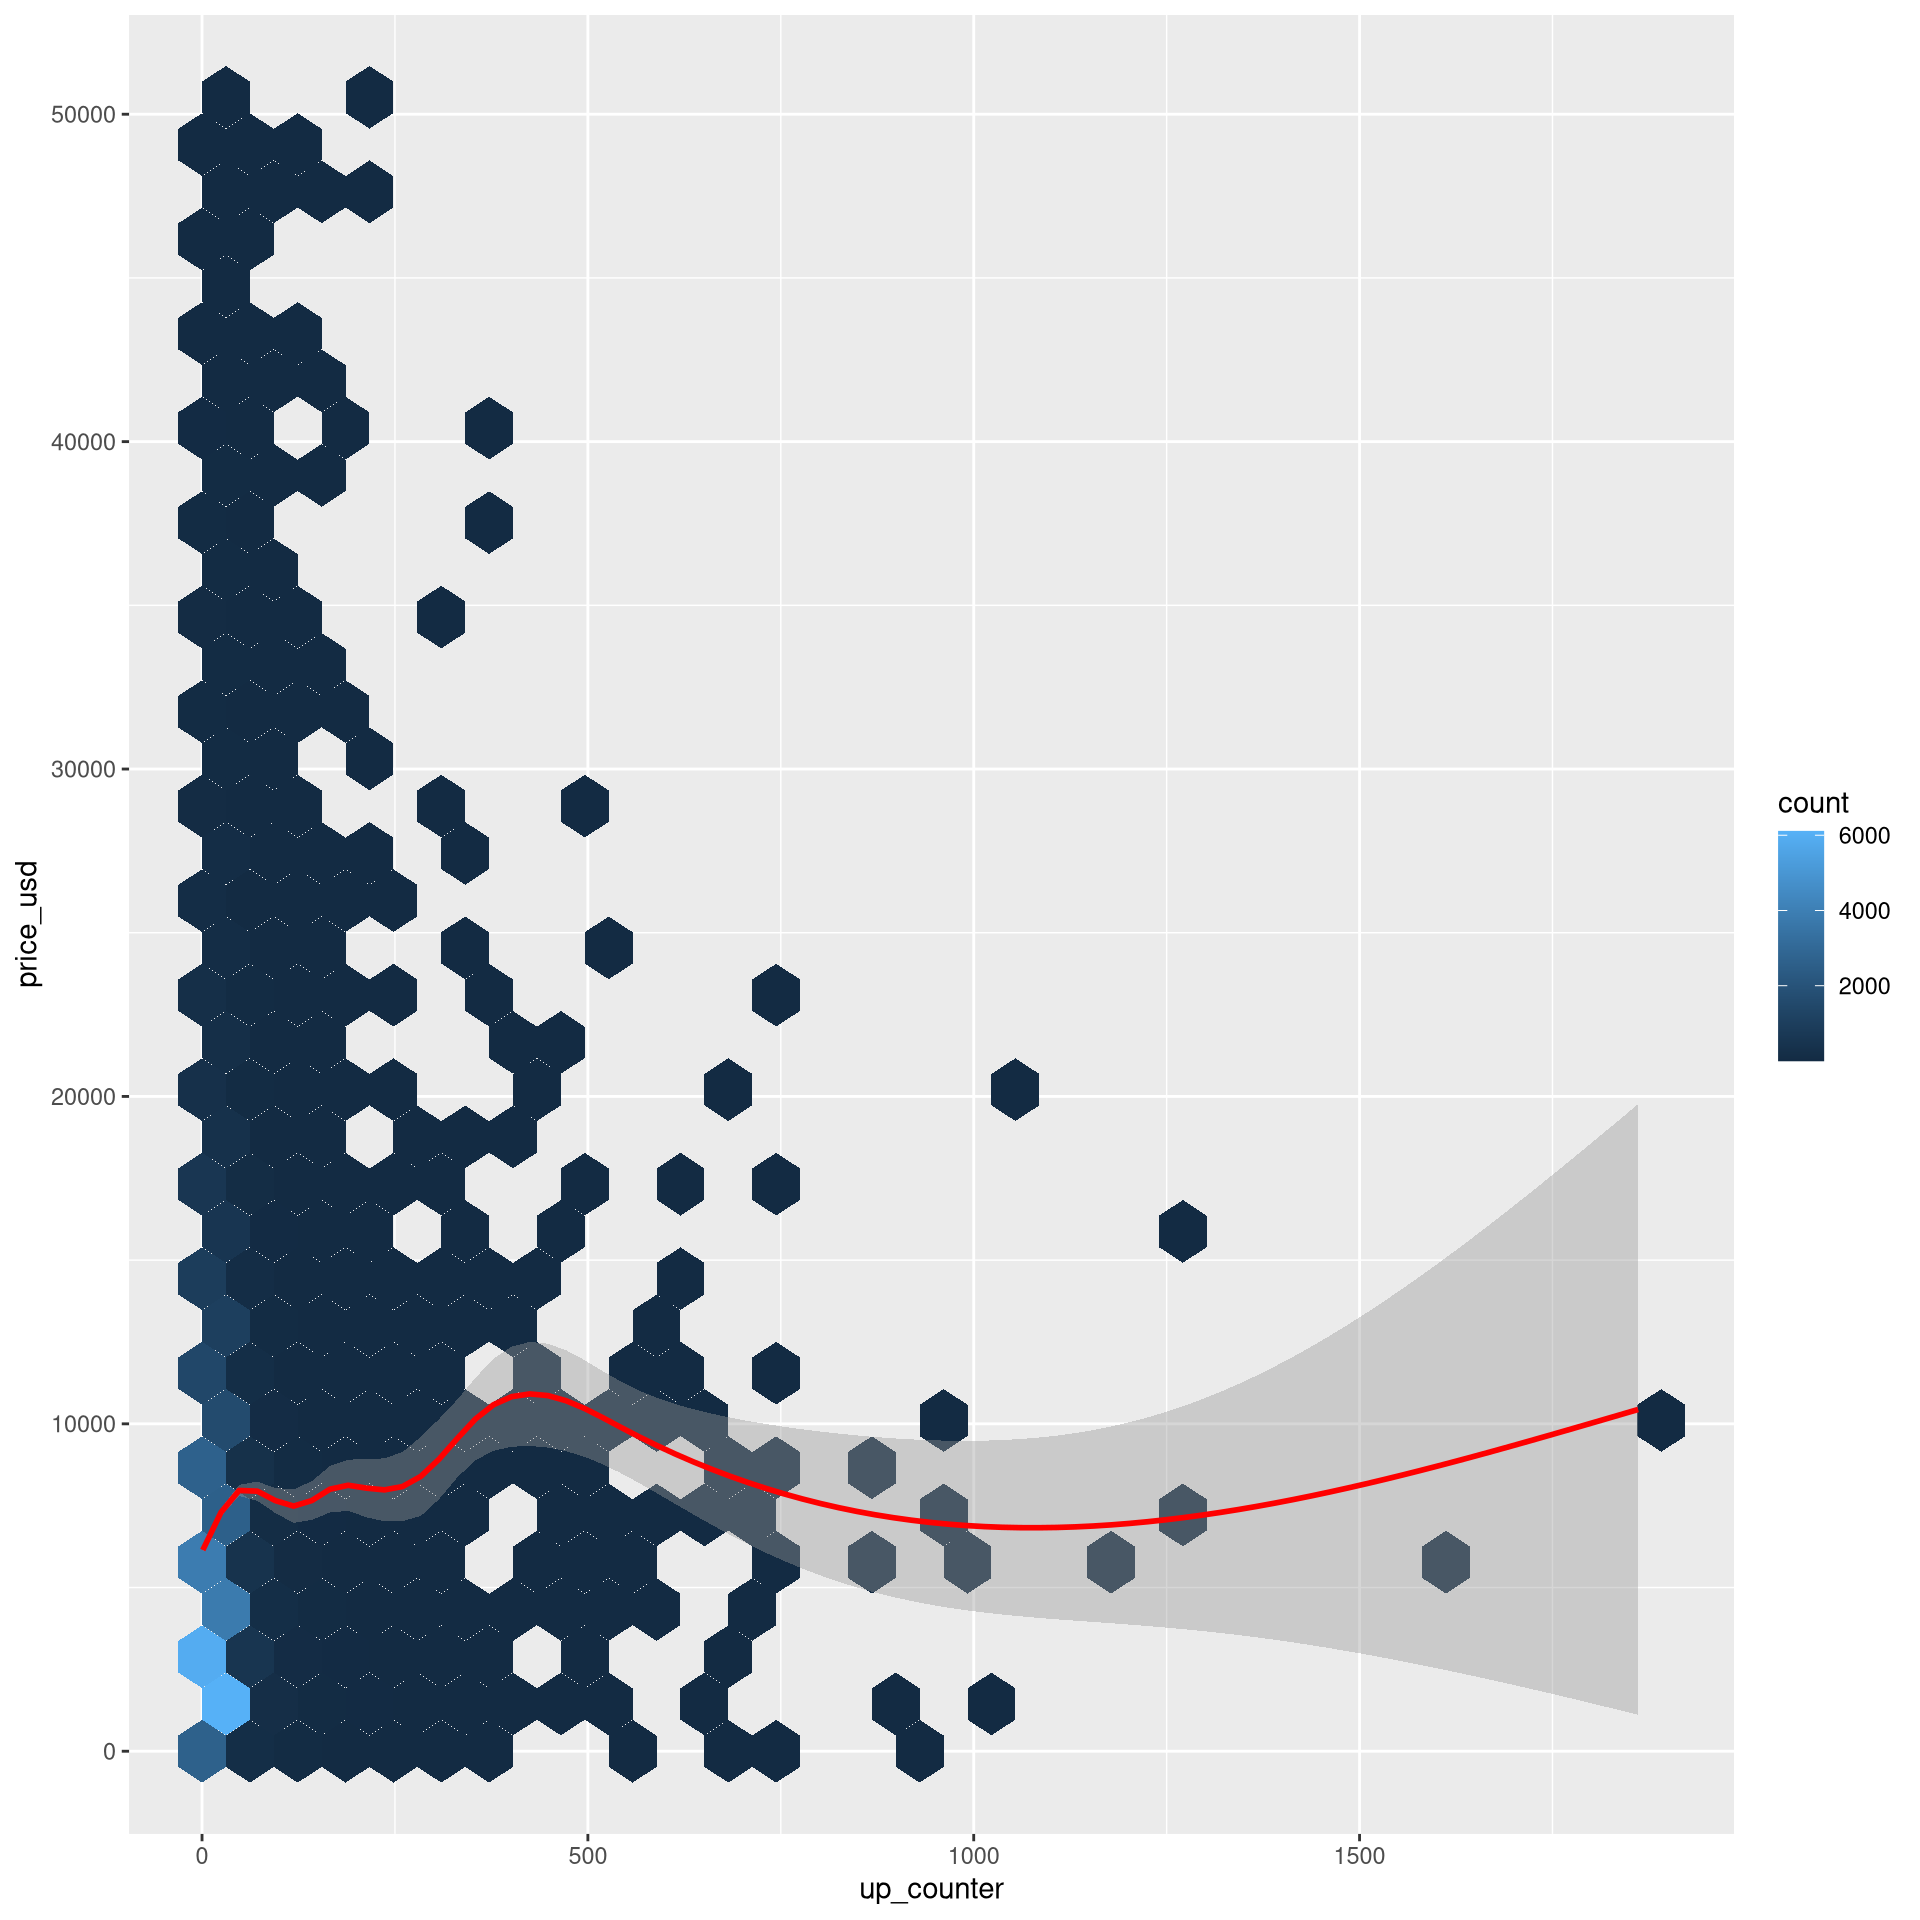
\includegraphics{Group1Report_files/figure-latex/upCounterPlot-1.pdf}

Looking at the scatterplot we see a possible positive correlation
although the variability of the data makes it hard for us to affirm this
prediction. To continue we will use the correlation test (since we are
dealing with continuous attributes) to check for a correlation between
number of up counts and price of a vehicle.

The hypotheses for the correlation test are the following:

H\textsubscript{0} =There does not exist a correlation between number of
up counts and vehicle price

H\textsubscript{a} = There does exist a correlation between number of up
counts and vehicle price

We will use 0.05 as our significance level. The results are the
following:

\begin{Shaded}
\begin{Highlighting}[]
\CommentTok{\# UpCounterCorrelation}
\FunctionTok{cor.test}\NormalTok{(cars\_edited}\SpecialCharTok{$}\NormalTok{up\_counter, cars\_edited}\SpecialCharTok{$}\NormalTok{price\_usd)}
\end{Highlighting}
\end{Shaded}

\begin{verbatim}
## 
##  Pearson's product-moment correlation
## 
## data:  cars_edited$up_counter and cars_edited$price_usd
## t = 11.352, df = 38488, p-value < 2.2e-16
## alternative hypothesis: true correlation is not equal to 0
## 95 percent confidence interval:
##  0.04780740 0.06772124
## sample estimates:
##        cor 
## 0.05777007
\end{verbatim}

Since the p-value is less than 0.05 we can conclude that Price and
number of up counts are correlated with a correlation coefficient of
0.05777007 and p-value of \textless{} 2.2e-16.

However, although they are correlated, we do see that the correlation
coefficient is very close to 0. Meaning that the correlation is almost
entirely negligible. If one were to use this as a predictor of price the
results would be poor.

Nevertheless, we will use linear regression to see how poor of an
indicator number of up counts really is. We will check the percentage of
accuracy of the linear regression line and graph the linear regression
line to provide useful insights.

\begin{Shaded}
\begin{Highlighting}[]
\CommentTok{\# Create LM}
\NormalTok{up\_counter\_on\_price }\OtherTok{\textless{}{-}} \FunctionTok{lm}\NormalTok{ (price\_usd }\SpecialCharTok{\textasciitilde{}}\NormalTok{ up\_counter, }\AttributeTok{data =}\NormalTok{ cars\_edited)}

\CommentTok{\#Finding how well this line fits the data}
\FunctionTok{summary}\NormalTok{(up\_counter\_on\_price)}
\end{Highlighting}
\end{Shaded}

\begin{verbatim}
## 
## Call:
## lm(formula = price_usd ~ up_counter, data = cars_edited)
## 
## Residuals:
##    Min     1Q Median     3Q    Max 
## -14558  -4502  -1852   2305  43438 
## 
## Coefficients:
##              Estimate Std. Error t value Pr(>|t|)    
## (Intercept) 6493.0457    34.9345  185.86   <2e-16 ***
## up_counter     8.5694     0.7548   11.35   <2e-16 ***
## ---
## Signif. codes:  0 '***' 0.001 '**' 0.01 '*' 0.05 '.' 0.1 ' ' 1
## 
## Residual standard error: 6413 on 38488 degrees of freedom
## Multiple R-squared:  0.003337,   Adjusted R-squared:  0.003311 
## F-statistic: 128.9 on 1 and 38488 DF,  p-value: < 2.2e-16
\end{verbatim}

\begin{Shaded}
\begin{Highlighting}[]
\CommentTok{\# R\^{}2 is extremely low which affirms that number of photos is not a good indicator of price. }

\FunctionTok{confint}\NormalTok{(up\_counter\_on\_price)}
\end{Highlighting}
\end{Shaded}

\begin{verbatim}
##                   2.5 %     97.5 %
## (Intercept) 6424.573138 6561.51822
## up_counter     7.089888   10.04893
\end{verbatim}

\begin{Shaded}
\begin{Highlighting}[]
\FunctionTok{sigma}\NormalTok{(up\_counter\_on\_price)}\SpecialCharTok{*}\DecValTok{100}\SpecialCharTok{/}\FunctionTok{mean}\NormalTok{(cars\_edited}\SpecialCharTok{$}\NormalTok{price\_usd)}
\end{Highlighting}
\end{Shaded}

\begin{verbatim}
## [1] 96.69137
\end{verbatim}

\begin{Shaded}
\begin{Highlighting}[]
\CommentTok{\# Our prediction error rate is extremely high (96.65168\%) which confirms to us that up\_counter is a terrible predictor of price(as we can see by the correlation test)}

\CommentTok{\#Scatter plot: up counter and price with regression line}
\FunctionTok{ggplot}\NormalTok{ (cars\_edited, }\FunctionTok{aes}\NormalTok{(}\AttributeTok{x=}\NormalTok{up\_counter, }\AttributeTok{y=}\NormalTok{price\_usd)) }\SpecialCharTok{+} \FunctionTok{geom\_point}\NormalTok{() }\SpecialCharTok{+} \FunctionTok{stat\_smooth}\NormalTok{(}\AttributeTok{method=}\NormalTok{lm)}
\end{Highlighting}
\end{Shaded}

\begin{verbatim}
## `geom_smooth()` using formula 'y ~ x'
\end{verbatim}

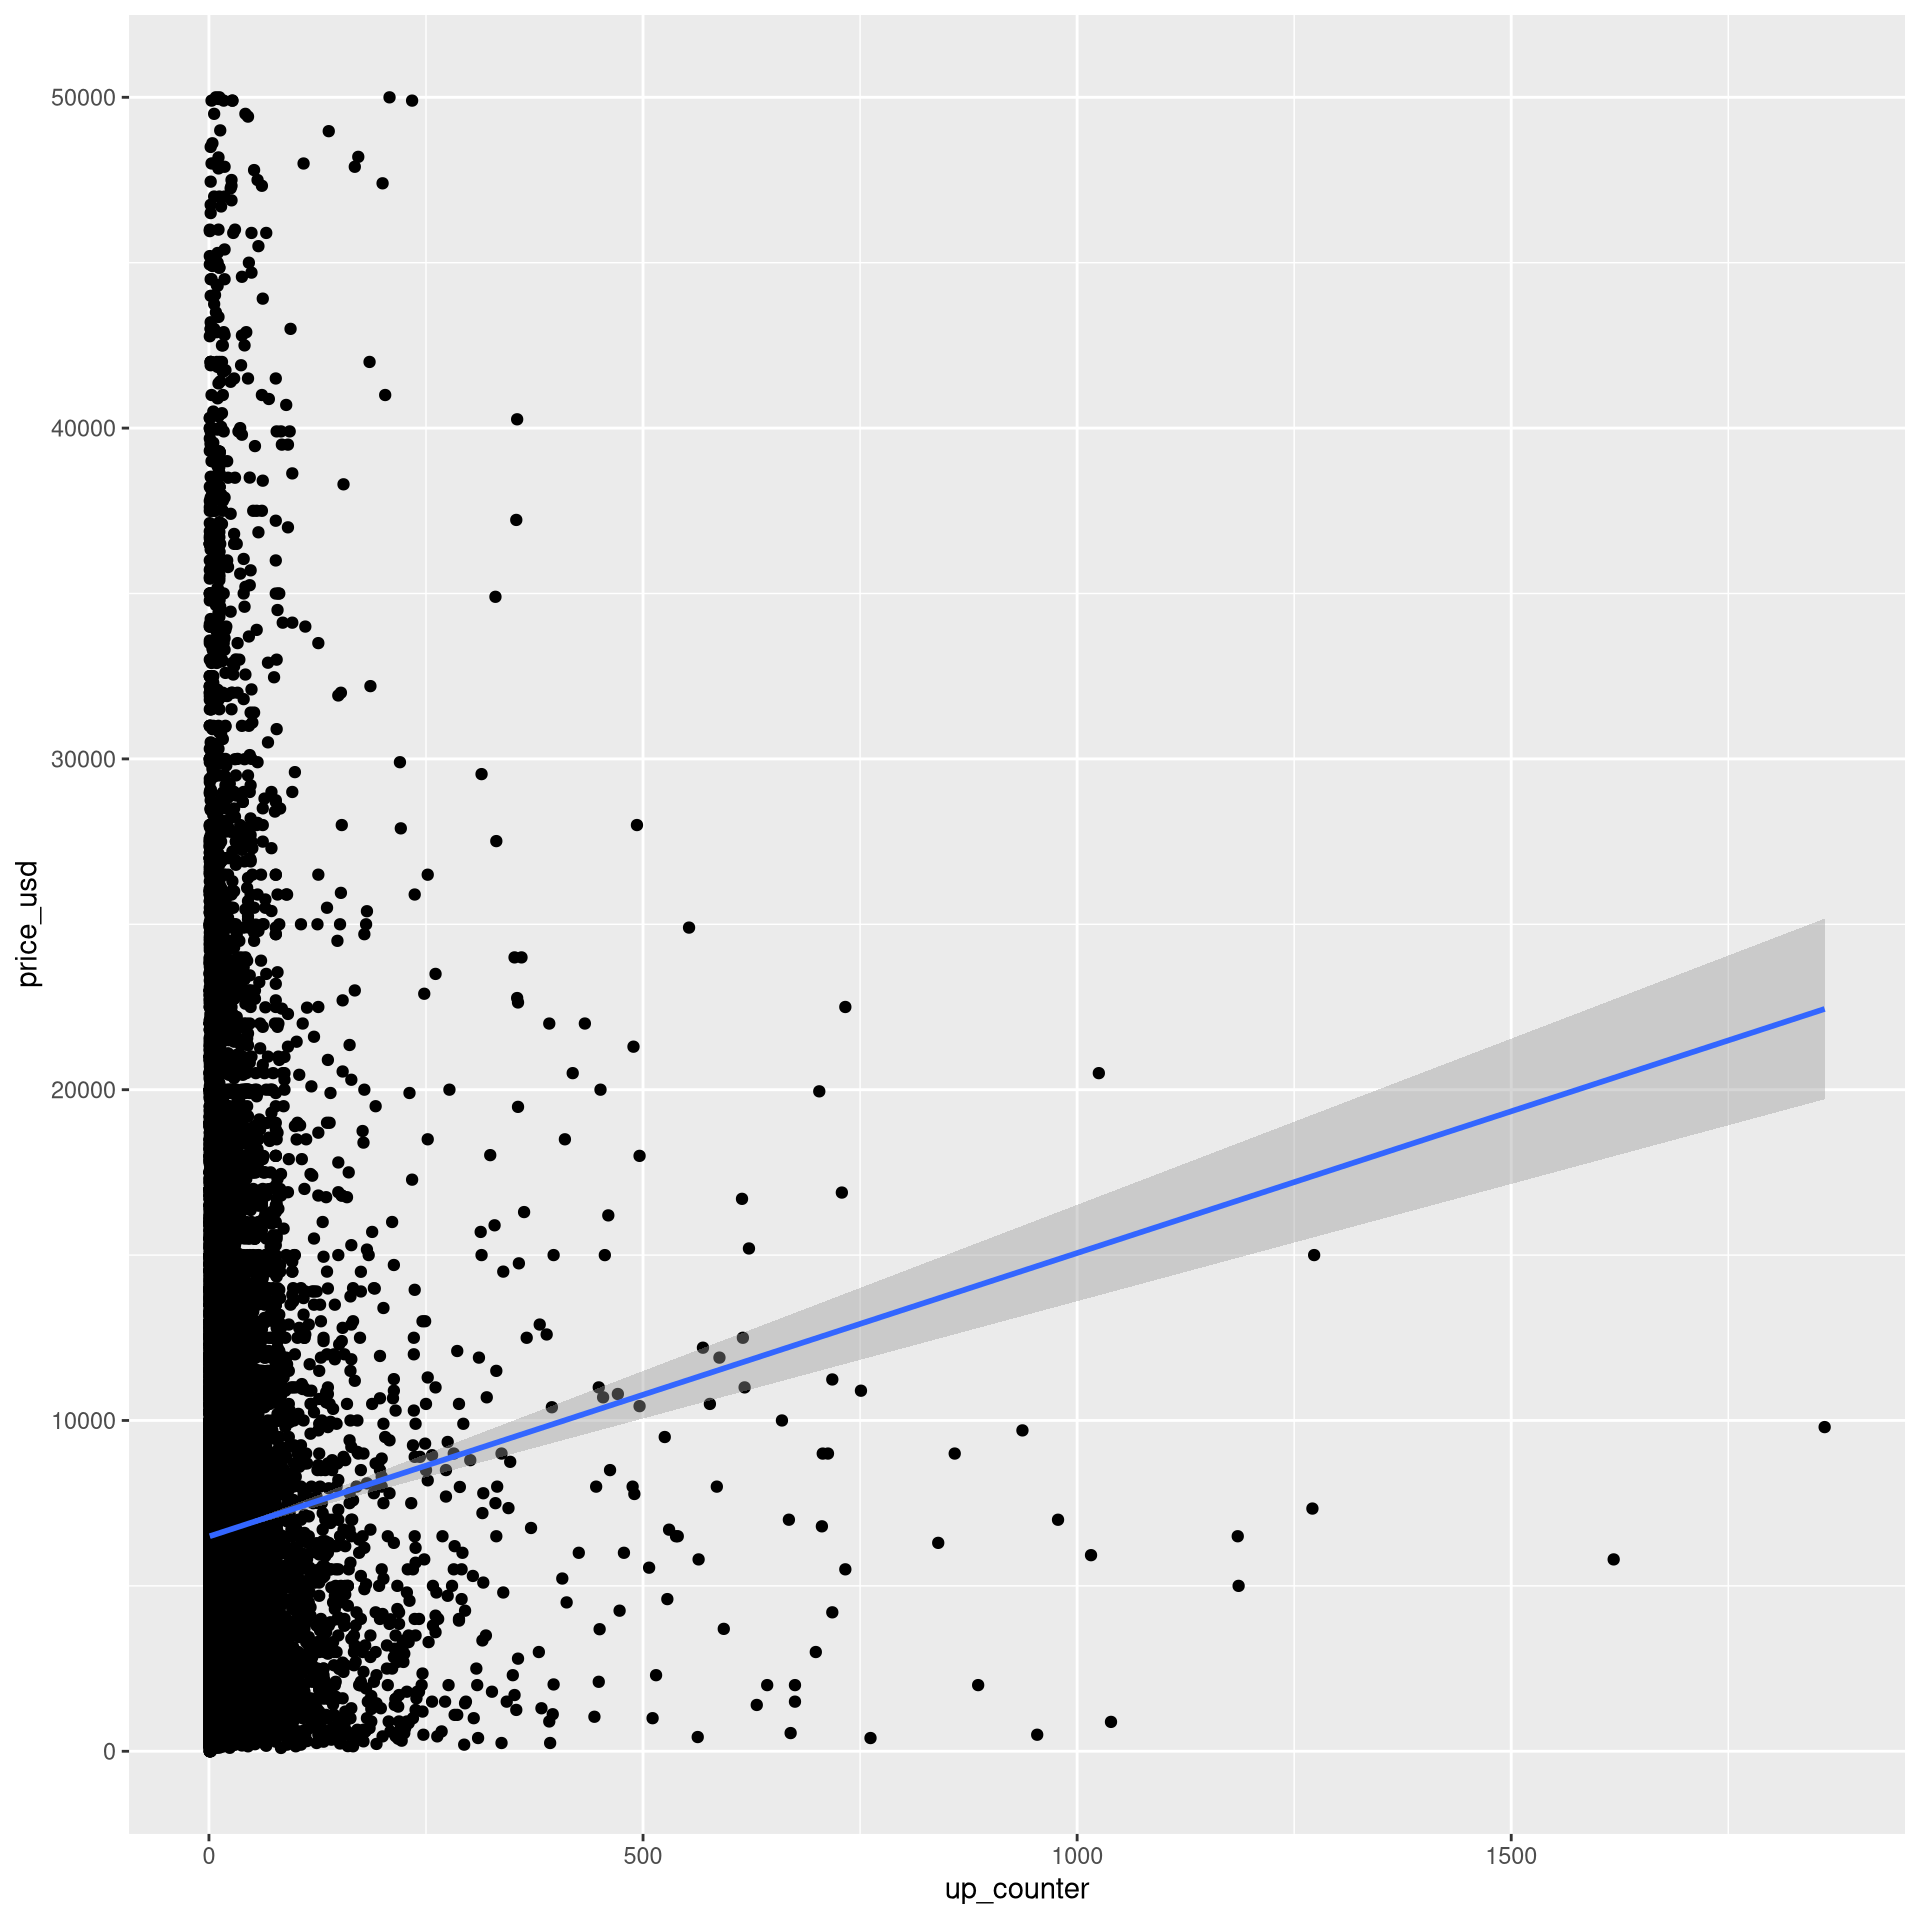
\includegraphics{Group1Report_files/figure-latex/UpCounterLM/Accuracy/Plot-1.pdf}

The R2 is 0.003311 which indicates that a low proportion of prices in
the data can be explained by the model. In other words, number of up
counts is a very poor indicator of price (we need more attributes in the
model). Also, the percentage error is 96.69137 which is ludicrously
high. This confirms how poor a model would be if it solely used number
of up counts to predict price.

\textbf{We can conclude there is a negligible positive correlation
between price and number of up counts.}

\begin{center}\rule{0.5\linewidth}{0.5pt}\end{center}

\hypertarget{q6-relationship-between-engine-type-and-body-type-what-is-the-impact-of-engine-type-and-body-type-on-the-selling-price}{%
\paragraph{\texorpdfstring{\textbf{Q6:} Relationship between Engine Type
and Body Type? What is the impact of Engine Type and Body Type on the
selling
price?}{Q6: Relationship between Engine Type and Body Type? What is the impact of Engine Type and Body Type on the selling price?}}\label{q6-relationship-between-engine-type-and-body-type-what-is-the-impact-of-engine-type-and-body-type-on-the-selling-price}}

\textbf{A: Sedan and Gasoline is the most common followed by Gasoline
and Hatchback. Engine Type and Body Type do have an impact on the
selling price, but the extend of this impact will need to be
investigated in our overall model.}

\textbf{Justification}:

To begin this question, it was important to have a working knowledge of
how body type and engine type related to one another. Initially a Mosaic
plot felt like the right graph to show relationships, but the quantity
of categories made a balloon plot much easy to read. The spacious nature
of the balloon plot greatly aided in gaining insights from the data and
pushed further investigation.

\begin{Shaded}
\begin{Highlighting}[]
\CommentTok{\# Balloon Plot}
\FunctionTok{ggplot}\NormalTok{(cars\_edited, }\FunctionTok{aes}\NormalTok{(body\_type, engine\_type)) }\SpecialCharTok{+} \FunctionTok{geom\_count}\NormalTok{()}
\end{Highlighting}
\end{Shaded}

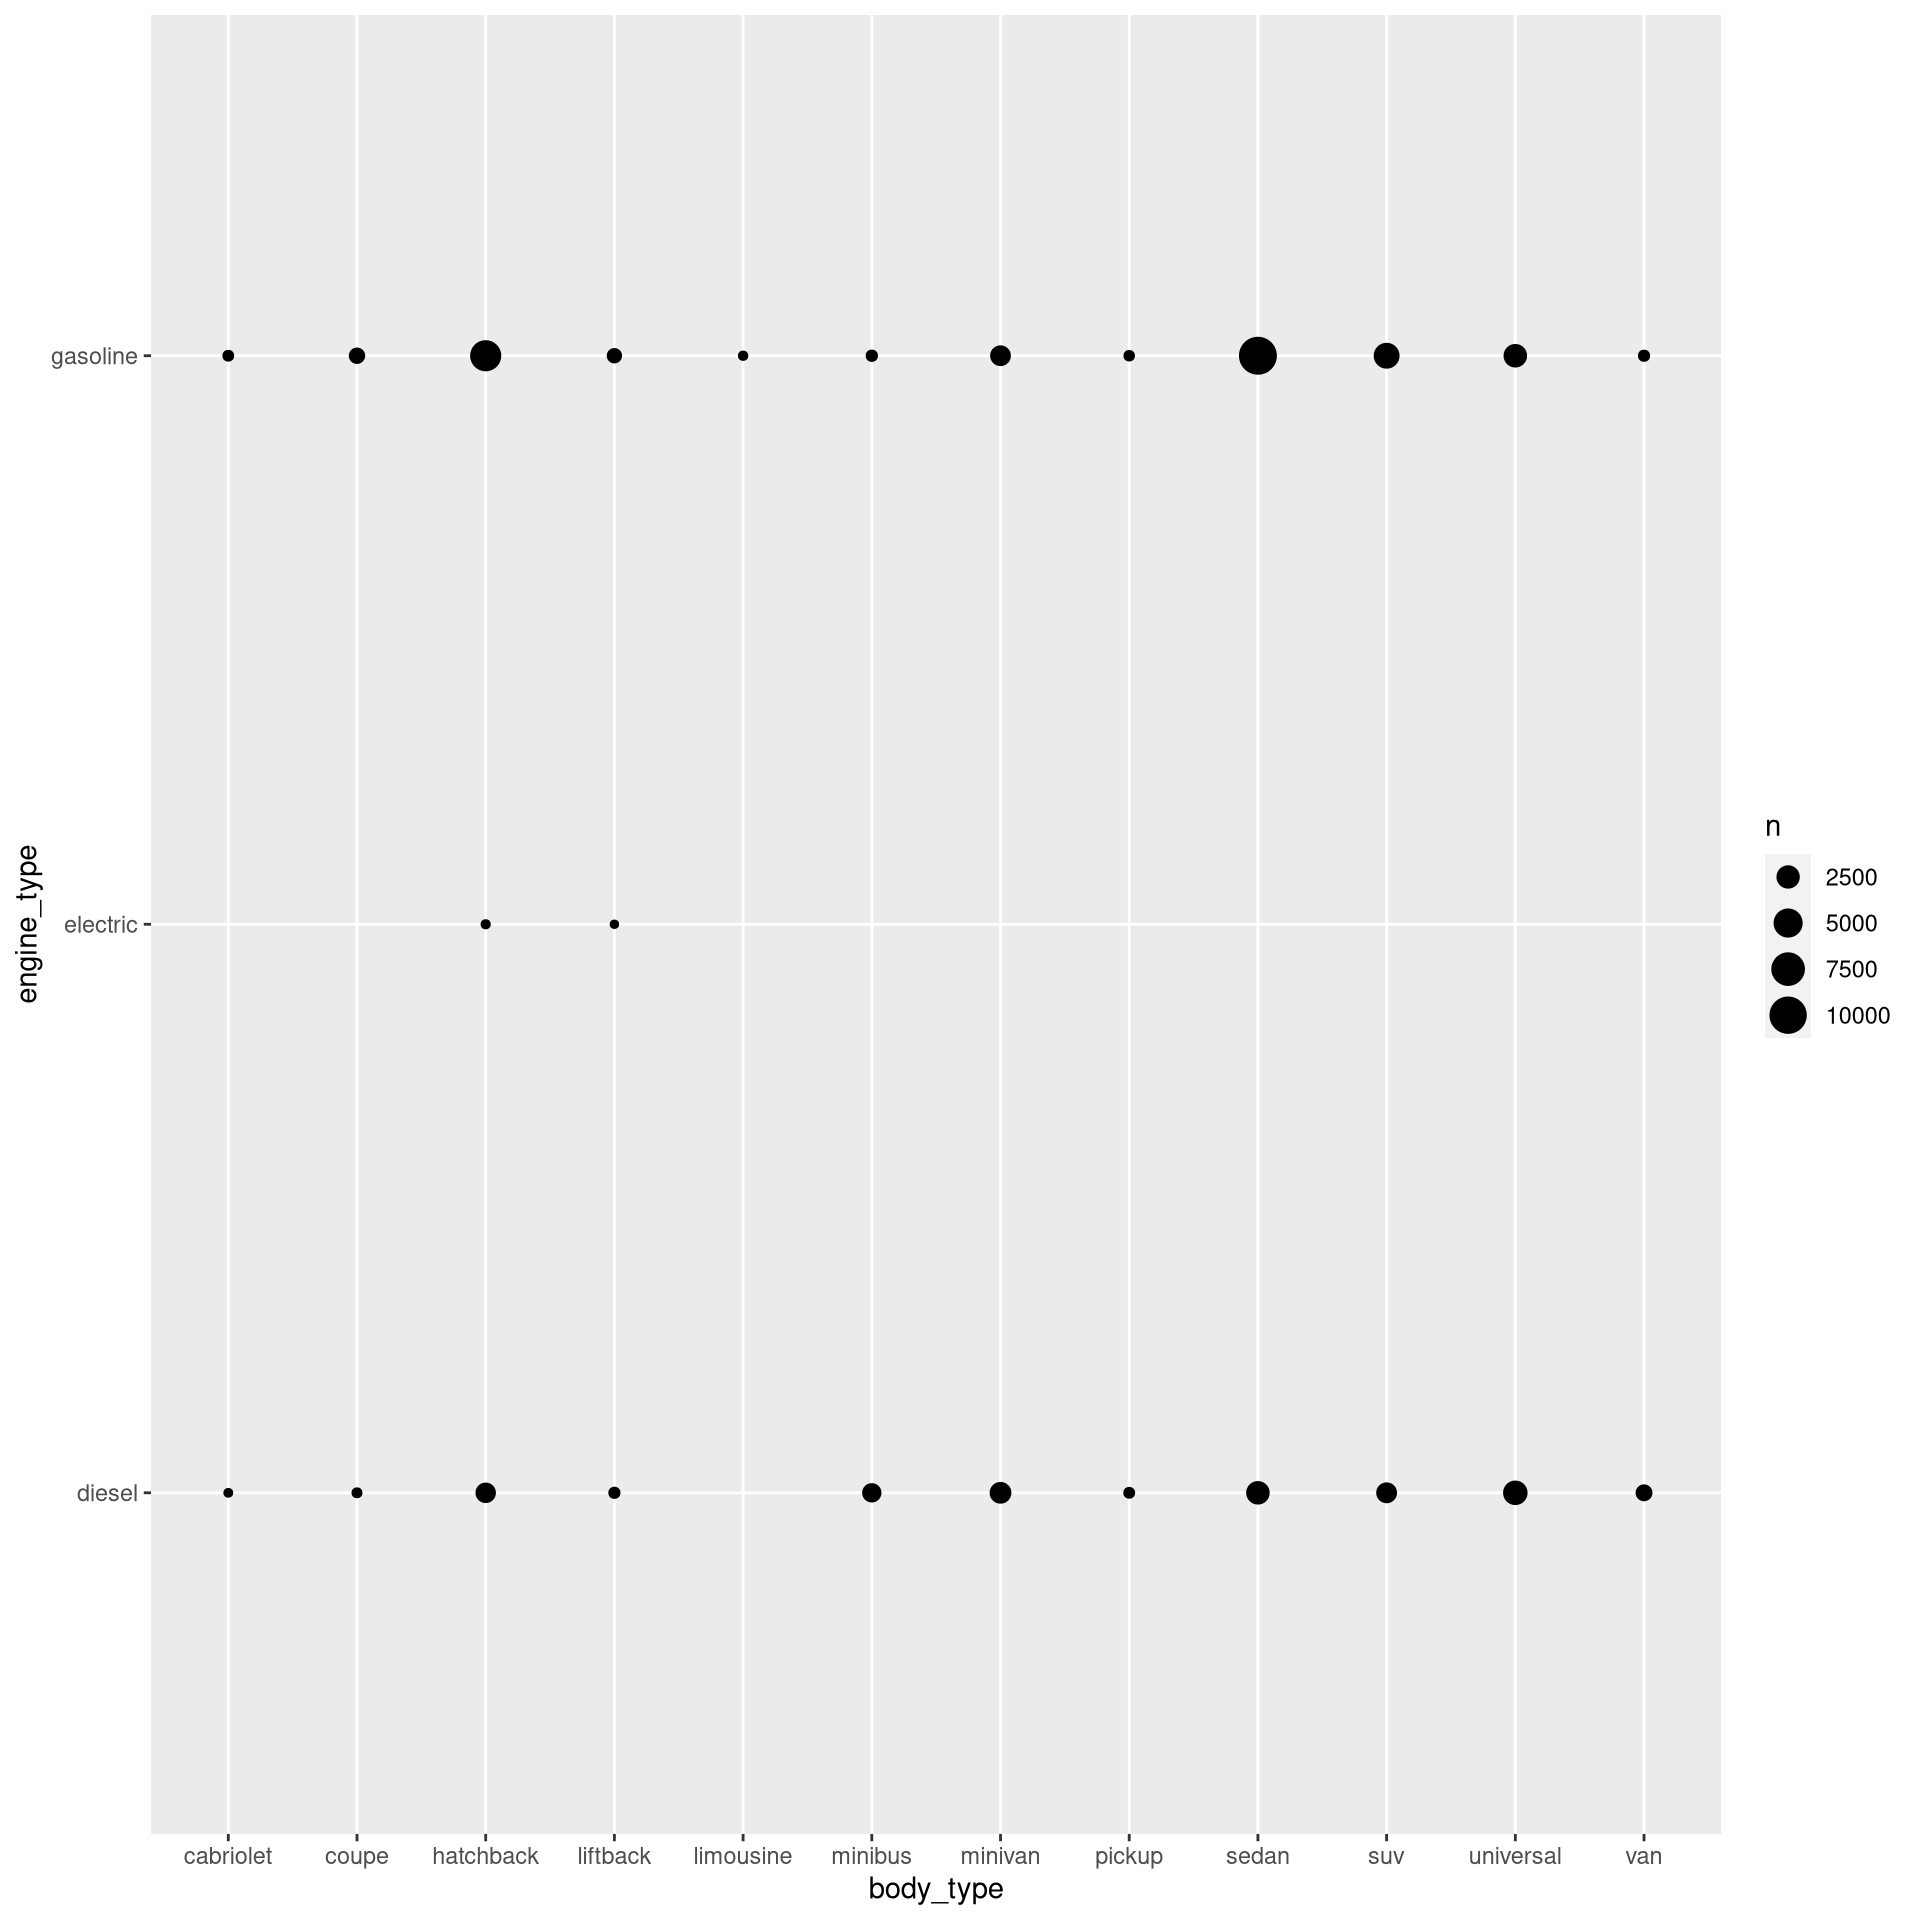
\includegraphics{Group1Report_files/figure-latex/EngBodyBalloonPlot-1.pdf}

Based on this Balloon plot we can see that several combinations of body
types and engine types do not exist. Furthermore, there seems to be
higher quantities of hatchbacks with gasoline engines and sedans with
gasoline engines. Nevertheless, visualization does not suffice in
proving any relationship. We shall proceed with a Chi-Square test for
more information. The reason for a Chi-Square test is that we are
attempting to analyze the frequency table of two categorical variables
(engine type and body type).

The hypotheses for the Chi-Square test are as follows:

H\textsubscript{0} = Engine Type and Body Type are independent

H\textsubscript{a} = Engine Type and Body Type are dependent

The test will be performed with 0.05 as our significance level. The
results are the following:

\begin{Shaded}
\begin{Highlighting}[]
\CommentTok{\#Chi{-}Square Test}
\NormalTok{engine\_body.data }\OtherTok{\textless{}{-}} \FunctionTok{table}\NormalTok{(cars\_edited}\SpecialCharTok{$}\NormalTok{body\_type, cars\_edited}\SpecialCharTok{$}\NormalTok{engine\_type)}
\FunctionTok{chisq.test}\NormalTok{(engine\_body.data)}
\end{Highlighting}
\end{Shaded}

\begin{verbatim}
## Warning in chisq.test(engine_body.data): Chi-squared approximation may be
## incorrect
\end{verbatim}

\begin{verbatim}
## 
##  Pearson's Chi-squared test
## 
## data:  engine_body.data
## X-squared = 6965.4, df = 22, p-value < 2.2e-16
\end{verbatim}

The result of the Chi-Square Test tells us that Engine Type and Body
Type are dependent.

We continue with a proportion table to give us an easy way of seeing the
distribution of engine type and body type.

\begin{Shaded}
\begin{Highlighting}[]
\CommentTok{\# Table}
\FunctionTok{prop.table}\NormalTok{(engine\_body.data)}\SpecialCharTok{*}\DecValTok{100}
\end{Highlighting}
\end{Shaded}

\begin{verbatim}
##            
##                   diesel     electric     gasoline
##   cabriolet  0.010392310  0.000000000  0.184463497
##   coupe      0.080540400  0.000000000  1.613406080
##   hatchback  4.081579631  0.020784619 15.757339569
##   liftback   0.249415433  0.005196155  1.176929072
##   limousine  0.000000000  0.000000000  0.031176929
##   minibus    3.273577553  0.000000000  0.280592362
##   minivan    5.081839439  0.000000000  4.292023902
##   pickup     0.192257729  0.000000000  0.142894258
##   sedan      6.635489738  0.000000000 27.079760977
##   suv        4.359573915  0.000000000  9.051701741
##   universal  7.622759158  0.000000000  6.677058976
##   van        1.847233048  0.000000000  0.252013510
\end{verbatim}

From the table we can clearly see that Hatchback and Gasoline as well as
Sedan and Gasoline are the most common combinations of the two variables
as we suspected from the balloon plot.

We continue by attempting to solve that second part of the question.
That is, what is the impact of Engine Type and Body Type on the selling
price?

The most effective method of solving this question is with the use of
the Two-Way Anova. The reason for the use of this test is because we are
attempting to evaluate the simultaneous effect of two grouping variables
(engine and body type) on a response variable(price).

The hypotheses for the Two-Way Anova test are:

H\textsubscript{o} = 1. There is no difference in the means of Engine
Type 2. There is no difference in the means of Body Type. 3. There is no
interaction between engine and body type

Ha = For cases 1 and 2 the means are not equal and for case 3 there is
an interaction between Engine and Body Type.

\begin{Shaded}
\begin{Highlighting}[]
\NormalTok{body\_engine\_type\_on\_price.aov }\OtherTok{\textless{}{-}} \FunctionTok{aov}\NormalTok{(price\_usd }\SpecialCharTok{\textasciitilde{}}\NormalTok{ engine\_type }\SpecialCharTok{*}\NormalTok{ body\_type, }\AttributeTok{data =}\NormalTok{ cars\_edited)}
\FunctionTok{summary}\NormalTok{(body\_engine\_type\_on\_price.aov)}
\end{Highlighting}
\end{Shaded}

\begin{verbatim}
##                          Df    Sum Sq   Mean Sq F value Pr(>F)    
## engine_type               2 1.301e+10 6.503e+09  204.12 <2e-16 ***
## body_type                11 3.457e+11 3.142e+10  986.32 <2e-16 ***
## engine_type:body_type    11 4.280e+09 3.891e+08   12.21 <2e-16 ***
## Residuals             38465 1.225e+12 3.186e+07                   
## ---
## Signif. codes:  0 '***' 0.001 '**' 0.01 '*' 0.05 '.' 0.1 ' ' 1
\end{verbatim}

Since the p-value is less than 0.05 for all three cases we can confirm
that there is a difference in the means of Engine Type, the means of
Body Type, and there is an interaction between Engine and Body Type.

To conclude our investigation, we will run the Tukey Honest Significant
Differences to perform the multiple pairwise-comparisons between the
means of groups to determine which groups are different and how they
differ.

\begin{Shaded}
\begin{Highlighting}[]
\CommentTok{\# Result omitted for brevity\textquotesingle{}s sake\}}
\CommentTok{\#Tukey HSD}
\FunctionTok{TukeyHSD}\NormalTok{(body\_engine\_type\_on\_price.aov)}
\DocumentationTok{\#\# Fit: aov(formula = price\_usd \textasciitilde{} engine\_type * body\_type, data = cars\_edited)}
\DocumentationTok{\#\# }
\DocumentationTok{\#\# $engine\_type}
\DocumentationTok{\#\#                         diff        lwr       upr p adj}
\DocumentationTok{\#\# electric{-}diesel    10052.532   5867.612 14237.452 1e{-}07}
\DocumentationTok{\#\# gasoline{-}diesel    {-}1175.359  {-}1318.298 {-}1032.420 0e+00}
\DocumentationTok{\#\# gasoline{-}electric {-}11227.891 {-}15412.002 {-}7043.779 0e+00}
\end{Highlighting}
\end{Shaded}

The Tukey Test results can be evaluated to gain more detailed
information on the relationship between price and Engine/Body Type.

\textbf{These tests confirm our that Engine Type and Body Type
significantly impact the selling price of a vehicle.}

\begin{center}\rule{0.5\linewidth}{0.5pt}\end{center}

\hypertarget{q7-what-is-the-most-popular-model-and-whether-we-can-conclude-that-the-popularity-of-a-model-has-a-direct-impact-on-the-price-of-a-vehicle}{%
\paragraph{\texorpdfstring{\textbf{Q7:} What is the most popular model
and whether we can conclude that the popularity of a model has a direct
impact on the price of a
vehicle?}{Q7: What is the most popular model and whether we can conclude that the popularity of a model has a direct impact on the price of a vehicle?}}\label{q7-what-is-the-most-popular-model-and-whether-we-can-conclude-that-the-popularity-of-a-model-has-a-direct-impact-on-the-price-of-a-vehicle}}

\textbf{A}: \textbf{The most popular is the Passat. Furthermore, the
popularity of a vehicle does seem to have an impact on the
average\_price of a vehicle. However, more attributes would be needed to
predict price.}

\textbf{Justification:}

The nature of the first part of the question informs us that we can
figure out the most popular model without a graph. To find the most
popular model we performed a count on every model and printed out the
result.

\begin{Shaded}
\begin{Highlighting}[]
\CommentTok{\# Finding out model popularity}
\NormalTok{models\_counted }\OtherTok{\textless{}{-}}\NormalTok{ cars\_edited }\SpecialCharTok{\%\textgreater{}\%} \FunctionTok{count}\NormalTok{(model\_name)}
\NormalTok{models\_counted }\SpecialCharTok{\%\textgreater{}\%} \FunctionTok{arrange}\NormalTok{(}\FunctionTok{desc}\NormalTok{(n))}
\end{Highlighting}
\end{Shaded}

\begin{verbatim}
## # A tibble: 1,118 x 2
##    model_name     n
##    <chr>      <int>
##  1 Passat      1422
##  2 Astra        751
##  3 Golf         707
##  4 A6           687
##  5 Mondeo       636
##  6 Vectra       565
##  7 Laguna       548
##  8 A4           505
##  9 406          415
## 10 Omega        387
## # ... with 1,108 more rows
\end{verbatim}

\textbf{From the table, the most popular model is the Passat.}

Now we go on to solve the next part of the question: Whether we can
conclude that the popularity of a model has a direct impact on the price
of a vehicle?

Since we are using a categorical factor and attempting to find its
impact on a continuous response variable, we will deploy the One-Way
Anova Test.

The hypotheses for the One-Way Anova test are:

H\textsubscript{o} = The means of the different models are the same

H\textsubscript{a} = At least one sample mean is not equal to the
others.

Also, the level of significance to be used with this test is 0.05.

We proceed by running the following code:

\begin{Shaded}
\begin{Highlighting}[]
\CommentTok{\# Do an Anova test to see if model\_name significantly impacts price of a vehicle}
\NormalTok{model\_price }\OtherTok{\textless{}{-}} \FunctionTok{aov}\NormalTok{(price\_usd }\SpecialCharTok{\textasciitilde{}}\NormalTok{ model\_name, }\AttributeTok{data =}\NormalTok{ cars\_edited)}
\FunctionTok{summary}\NormalTok{(model\_price)}
\end{Highlighting}
\end{Shaded}

\begin{verbatim}
##                Df    Sum Sq   Mean Sq F value Pr(>F)    
## model_name   1117 9.775e+11 875117268   53.54 <2e-16 ***
## Residuals   37372 6.109e+11  16346307                   
## ---
## Signif. codes:  0 '***' 0.001 '**' 0.01 '*' 0.05 '.' 0.1 ' ' 1
\end{verbatim}

Since the p-value is less than 0.05 we can conclude that the model\_name
does have a significant impact on the price of a vehicle.

We continue our investigation by attempting to see how effective
model\_name is in predicting the price of a vehicle. To do this we will
use a Simple Linear Regression model as follows:

\begin{Shaded}
\begin{Highlighting}[]
\CommentTok{\#Taking the linear regression}
\NormalTok{modelPrice }\OtherTok{\textless{}{-}} \FunctionTok{lm}\NormalTok{ (price\_usd }\SpecialCharTok{\textasciitilde{}}\NormalTok{ model\_name, }\AttributeTok{data =}\NormalTok{ cars\_edited)}
\end{Highlighting}
\end{Shaded}

\begin{Shaded}
\begin{Highlighting}[]
\CommentTok{\# Result omitted for brevity\textquotesingle{}s sake}
\CommentTok{\# Making sure the linear regression line matches the model}
\FunctionTok{summary}\NormalTok{(modelPrice)}
\DocumentationTok{\#\# Residual standard error: 4043 on 37372 degrees of freedom}
\DocumentationTok{\#\# Multiple R{-}squared:  0.6154, Adjusted R{-}squared:  0.6039 }
\DocumentationTok{\#\# F{-}statistic: 53.54 on 1117 and 37372 DF,  p{-}value: \textless{} 2.2e{-}16}
\end{Highlighting}
\end{Shaded}

The R2 is 0.6039 which indicates that a relatively large proportion of
prices in the data can be explained by the model. Although more
attributes will aid in predicting prices, we can confirm that there is
significant usefulness in using the model\_name attribute in our future
models.

We continue by assessing the error of our model to get a better picture
of the model's accuracy.

\begin{Shaded}
\begin{Highlighting}[]
\CommentTok{\# Result omitted for brevity\textquotesingle{}s sake}
\FunctionTok{confint}\NormalTok{(modelPrice)}
\end{Highlighting}
\end{Shaded}

\begin{Shaded}
\begin{Highlighting}[]
\FunctionTok{sigma}\NormalTok{(modelPrice)}\SpecialCharTok{*}\DecValTok{100}\SpecialCharTok{/}\FunctionTok{mean}\NormalTok{(cars\_edited}\SpecialCharTok{$}\NormalTok{price\_usd)}
\end{Highlighting}
\end{Shaded}

\begin{verbatim}
## [1] 60.95455
\end{verbatim}

Our prediction error rate is lower than for other attributes
(60.95455\%) which confirms to us that model name is a better predictor
of price. Nevertheless, a prediction error of 60.95455\% tells us that
for prediction we will need more attributes.

\textbf{This analysis concludes that the popularity of a vehicle does
seem to have an impact on the average\_price of a vehicle. However, more
attributes would be needed to predict price.}

\begin{center}\rule{0.5\linewidth}{0.5pt}\end{center}

\hypertarget{q8-what-is-the-average-age-of-each-vehicle-manufacturer-and-whether-the-manufacturer-changes-how-the-production-year-impacts-the-price}{%
\paragraph{\texorpdfstring{\textbf{Q8:} What is the average age of each
vehicle manufacturer and whether the manufacturer changes how the
production year impacts the
price?}{Q8: What is the average age of each vehicle manufacturer and whether the manufacturer changes how the production year impacts the price?}}\label{q8-what-is-the-average-age-of-each-vehicle-manufacturer-and-whether-the-manufacturer-changes-how-the-production-year-impacts-the-price}}

\textbf{A: The average age of each manufacturer can be found using some
data transformation. Furthermore, the manufacturer does influence how
production year changes the price of a vehicle.}

\textbf{Justification:}

Prior to working on this question, it would be useful to have some sort
of visual understanding of our data. To accomplish this, we will use a
scatter plat with facet wrap to show the distribution of years for each
manufacturer.

\begin{Shaded}
\begin{Highlighting}[]
\CommentTok{\#Scatter plot: Year produced by price and colored by manufacturer name}
\FunctionTok{ggplot}\NormalTok{(cars\_edited, }\FunctionTok{aes}\NormalTok{(}\AttributeTok{x =}\NormalTok{ year\_produced, }\AttributeTok{y =}\NormalTok{ price\_usd)) }\SpecialCharTok{+} \FunctionTok{geom\_hex}\NormalTok{() }\SpecialCharTok{+} \FunctionTok{facet\_wrap}\NormalTok{(}\SpecialCharTok{\textasciitilde{}}\NormalTok{ manufacturer\_name)}
\end{Highlighting}
\end{Shaded}

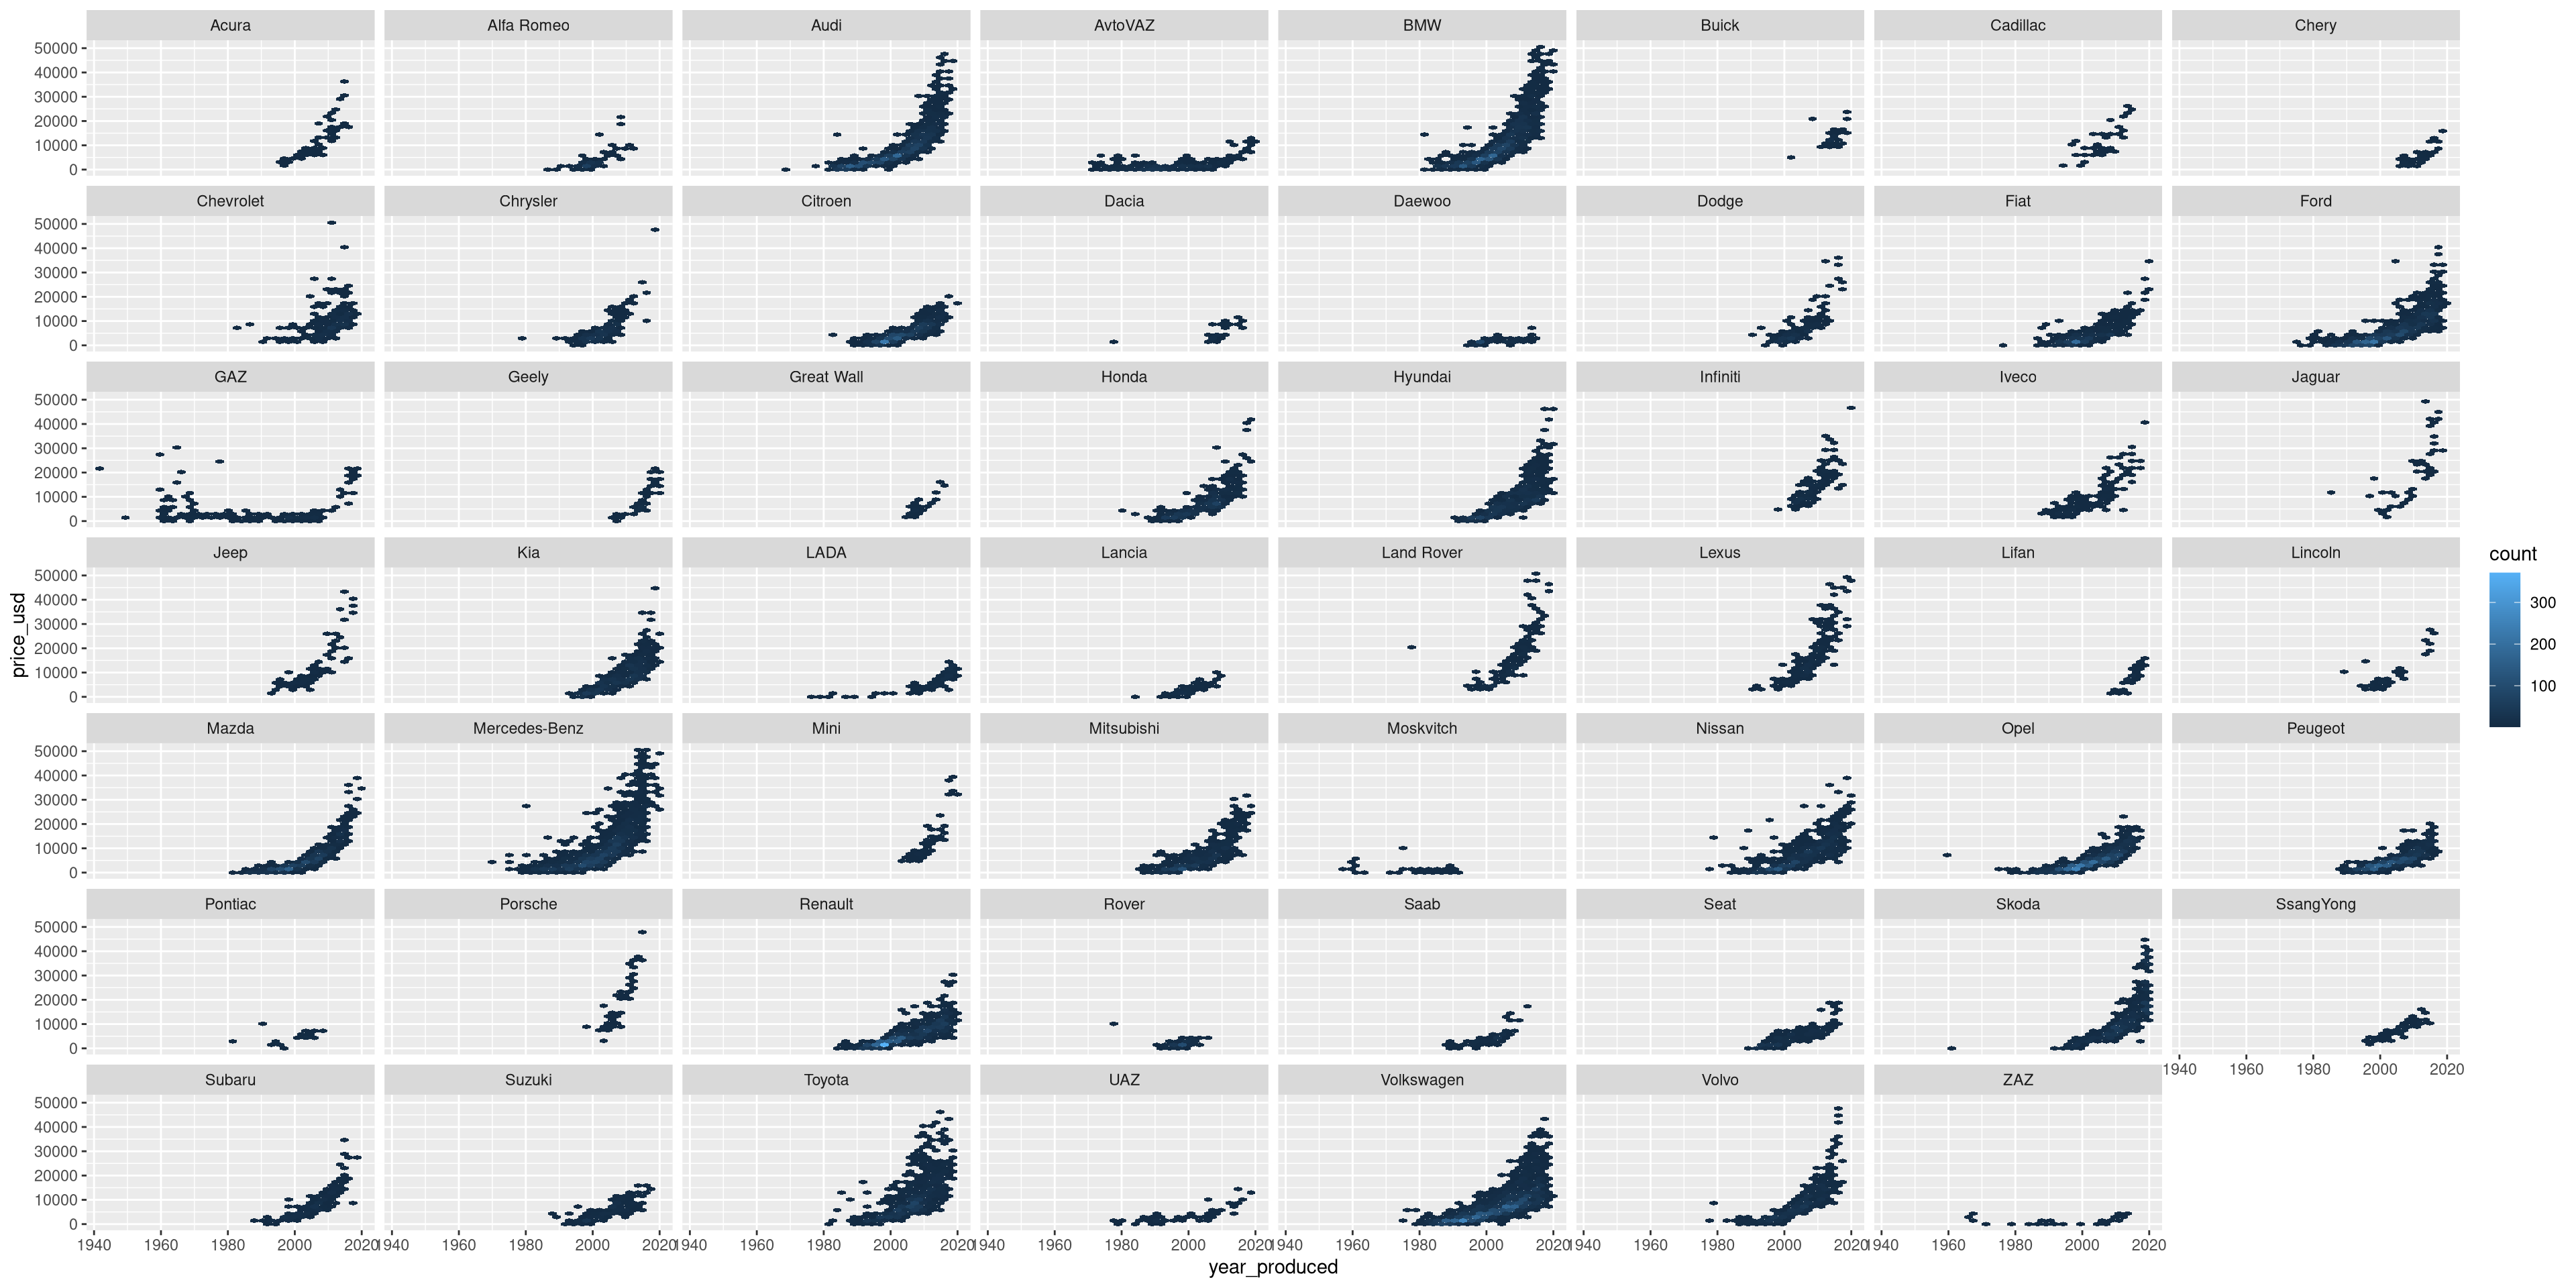
\includegraphics{Group1Report_files/figure-latex/ScatterPlotFacetHex-1.pdf}

Upon looking at the graph, visualization is not the way to solve this
question. Nevertheless, the graphs seem to follow a similar pattern;
more newer cars exist, and they are more expensive.

To solve for the average age of each manufacturer we will perform a data
transformation as follows:

\begin{Shaded}
\begin{Highlighting}[]
\CommentTok{\#Group cars by manufacturer name}
\NormalTok{manufacturer\_year }\OtherTok{\textless{}{-}} \FunctionTok{group\_by}\NormalTok{(cars\_edited, manufacturer\_name)}

\CommentTok{\#Summarize the manufacturer years average}
\NormalTok{manufacturer\_year\_averages }\OtherTok{\textless{}{-}} \FunctionTok{summarise}\NormalTok{(manufacturer\_year, }\AttributeTok{average =} \FunctionTok{mean}\NormalTok{(year\_produced, }\AttributeTok{na.rm =} \ConstantTok{TRUE}\NormalTok{))}
\CommentTok{\# 1) Average age of each vehicle manufacturer}
\NormalTok{manufacturer\_year\_averages }\SpecialCharTok{\%\textgreater{}\%} \FunctionTok{arrange}\NormalTok{(}\FunctionTok{desc}\NormalTok{(average))}
\end{Highlighting}
\end{Shaded}

\begin{verbatim}
## # A tibble: 55 x 2
##    manufacturer_name average
##    <chr>               <dbl>
##  1 Lifan               2015.
##  2 Buick               2014.
##  3 Geely               2014.
##  4 LADA                2014.
##  5 Skoda               2013.
##  6 Mini                2011.
##  7 Chevrolet           2011.
##  8 Chery               2011.
##  9 Great Wall          2009.
## 10 Dacia               2009.
## # ... with 45 more rows
\end{verbatim}

Observing the results of the summary the manufacturers with the newest
car averages are Lifan, Buick, Geely, and LADA.

Next, we continue with the second part of the question: Whether the
manufacturer changes how the production year impacts the price?

To solve this question, we will be using the Two-Way Anova. The Two-Way
Anova is used because we are attempting to evaluate the simultaneous
effect of Manufacturer and Year Produced on price.

The hypotheses for the Two-Way Anova test are:

H\textsubscript{o} = 1. There is no difference in the means of
Manufacturer. There is no difference in the means of Year Produced. 3.
There is no interaction between Manufacturer and Year Produced

Ha = For cases 1 and 2 the means are not equal and for case 3 there is
an interaction between Manufacturer and Year Produced.

For this test we will be using 0.05 as our level of significance. The
results are thus:

\begin{Shaded}
\begin{Highlighting}[]
\CommentTok{\# Do an Anova test to see if year produced significantly impacts price of a vehicle}
\NormalTok{manufacturer\_price }\OtherTok{\textless{}{-}} \FunctionTok{aov}\NormalTok{(price\_usd }\SpecialCharTok{\textasciitilde{}}\NormalTok{ manufacturer\_name }\SpecialCharTok{*}\NormalTok{ year\_produced, }\AttributeTok{data =}\NormalTok{ cars\_edited)}
\FunctionTok{summary}\NormalTok{(manufacturer\_price)}
\end{Highlighting}
\end{Shaded}

\begin{verbatim}
##                                    Df    Sum Sq   Mean Sq F value Pr(>F)    
## manufacturer_name                  54 2.917e+11 5.402e+09   428.4 <2e-16 ***
## year_produced                       1 6.854e+11 6.854e+11 54355.5 <2e-16 ***
## manufacturer_name:year_produced    54 1.273e+11 2.357e+09   186.9 <2e-16 ***
## Residuals                       38380 4.840e+11 1.261e+07                   
## ---
## Signif. codes:  0 '***' 0.001 '**' 0.01 '*' 0.05 '.' 0.1 ' ' 1
\end{verbatim}

In our results we can see that the p-value \textless{} 0.05 for each of
our 3 cases. In other words, there is a difference in the means of
Manufacturer, the means of Year Produced, and there is an interaction
between Manufacturer and Year Produced. \textbf{The manufacturer does
change how the production year affects the selling price.}

Now that we know that Manufacturer and Year Produced impact the price of
our vehicle, it important to see how well of a model we can produce
given these two attributes. To do this we will use the Multiple Linear
Regression Model.

\begin{Shaded}
\begin{Highlighting}[]
\CommentTok{\#Taking the linear regression}
\NormalTok{ManufyearPrice }\OtherTok{\textless{}{-}} \FunctionTok{lm}\NormalTok{ (price\_usd }\SpecialCharTok{\textasciitilde{}}\NormalTok{ manufacturer\_name }\SpecialCharTok{+}\NormalTok{ year\_produced, }\AttributeTok{data =}\NormalTok{ cars\_edited)}

\CommentTok{\#Making sure the linear regression line matches the model}
\FunctionTok{summary}\NormalTok{(ManufyearPrice)}
\end{Highlighting}
\end{Shaded}

\begin{verbatim}
## 
## Call:
## lm(formula = price_usd ~ manufacturer_name + year_produced, data = cars_edited)
## 
## Residuals:
##    Min     1Q Median     3Q    Max 
## -14133  -2147   -519   1134  44499 
## 
## Coefficients:
##                                  Estimate Std. Error  t value Pr(>|t|)    
## (Intercept)                    -1.140e+06  5.573e+03 -204.505  < 2e-16 ***
## manufacturer_nameAlfa Romeo    -5.591e+03  5.642e+02   -9.910  < 2e-16 ***
## manufacturer_nameAudi          -1.586e+03  4.978e+02   -3.187  0.00144 ** 
## manufacturer_nameAvtoVAZ       -3.893e+03  5.247e+02   -7.421 1.19e-13 ***
## manufacturer_nameBMW           -6.043e+02  4.972e+02   -1.215  0.22420    
## manufacturer_nameBuick         -4.103e+03  7.614e+02   -5.388 7.16e-08 ***
## manufacturer_nameCadillac      -1.036e+03  7.816e+02   -1.326  0.18499    
## manufacturer_nameChery         -1.024e+04  7.178e+02  -14.260  < 2e-16 ***
## manufacturer_nameChevrolet     -5.946e+03  5.268e+02  -11.287  < 2e-16 ***
## manufacturer_nameChrysler      -4.698e+03  5.291e+02   -8.879  < 2e-16 ***
## manufacturer_nameCitroen       -6.049e+03  5.013e+02  -12.068  < 2e-16 ***
## manufacturer_nameDacia         -8.635e+03  7.145e+02  -12.085  < 2e-16 ***
## manufacturer_nameDaewoo        -7.848e+03  5.596e+02  -14.023  < 2e-16 ***
## manufacturer_nameDodge         -5.002e+03  5.428e+02   -9.215  < 2e-16 ***
## manufacturer_nameFiat          -5.770e+03  5.105e+02  -11.301  < 2e-16 ***
## manufacturer_nameFord          -4.785e+03  4.974e+02   -9.621  < 2e-16 ***
## manufacturer_nameGAZ            2.130e+03  5.686e+02    3.746  0.00018 ***
## manufacturer_nameGeely         -8.969e+03  6.822e+02  -13.149  < 2e-16 ***
## manufacturer_nameGreat Wall    -7.699e+03  8.263e+02   -9.317  < 2e-16 ***
## manufacturer_nameHonda         -4.274e+03  5.109e+02   -8.366  < 2e-16 ***
## manufacturer_nameHyundai       -4.627e+03  5.052e+02   -9.159  < 2e-16 ***
## manufacturer_nameInfiniti       5.880e+02  5.824e+02    1.010  0.31262    
## manufacturer_nameIveco         -2.139e+02  5.963e+02   -0.359  0.71978    
## manufacturer_nameJaguar         4.243e+03  7.356e+02    5.768 8.06e-09 ***
## manufacturer_nameJeep          -4.869e+02  6.242e+02   -0.780  0.43541    
## manufacturer_nameKia           -4.973e+03  5.083e+02   -9.782  < 2e-16 ***
## manufacturer_nameLADA          -9.049e+03  5.918e+02  -15.290  < 2e-16 ***
## manufacturer_nameLancia        -5.546e+03  6.436e+02   -8.616  < 2e-16 ***
## manufacturer_nameLand Rover     2.458e+03  5.722e+02    4.295 1.75e-05 ***
## manufacturer_nameLexus          3.756e+03  5.618e+02    6.686 2.33e-11 ***
## manufacturer_nameLifan         -9.028e+03  7.615e+02  -11.856  < 2e-16 ***
## manufacturer_nameLincoln       -6.532e+02  8.264e+02   -0.791  0.42924    
## manufacturer_nameMazda         -4.846e+03  5.032e+02   -9.631  < 2e-16 ***
## manufacturer_nameMercedes-Benz -2.389e+02  4.983e+02   -0.479  0.63163    
## manufacturer_nameMini          -1.706e+03  6.892e+02   -2.475  0.01332 *  
## manufacturer_nameMitsubishi    -4.406e+03  5.090e+02   -8.655  < 2e-16 ***
## manufacturer_nameMoskvitch      4.373e+03  7.323e+02    5.972 2.37e-09 ***
## manufacturer_nameNissan        -4.452e+03  5.027e+02   -8.856  < 2e-16 ***
## manufacturer_nameOpel          -5.383e+03  4.969e+02  -10.832  < 2e-16 ***
## manufacturer_namePeugeot       -5.964e+03  4.994e+02  -11.942  < 2e-16 ***
## manufacturer_namePontiac       -4.690e+03  7.874e+02   -5.956 2.60e-09 ***
## manufacturer_namePorsche        5.437e+03  7.083e+02    7.676 1.68e-14 ***
## manufacturer_nameRenault       -5.894e+03  4.975e+02  -11.848  < 2e-16 ***
## manufacturer_nameRover         -5.704e+03  5.562e+02  -10.256  < 2e-16 ***
## manufacturer_nameSaab          -4.979e+03  6.233e+02   -7.988 1.41e-15 ***
## manufacturer_nameSeat          -5.163e+03  5.420e+02   -9.525  < 2e-16 ***
## manufacturer_nameSkoda         -2.145e+03  5.062e+02   -4.237 2.27e-05 ***
## manufacturer_nameSsangYong     -4.715e+03  6.650e+02   -7.090 1.37e-12 ***
## manufacturer_nameSubaru        -3.727e+03  5.438e+02   -6.854 7.28e-12 ***
## manufacturer_nameSuzuki        -5.732e+03  5.559e+02  -10.312  < 2e-16 ***
## manufacturer_nameToyota        -2.302e+03  5.037e+02   -4.570 4.90e-06 ***
## manufacturer_nameUAZ           -4.713e+03  6.756e+02   -6.977 3.06e-12 ***
## manufacturer_nameVolkswagen    -3.251e+03  4.949e+02   -6.570 5.10e-11 ***
## manufacturer_nameVolvo         -2.688e+03  5.129e+02   -5.240 1.61e-07 ***
## manufacturer_nameZAZ           -5.519e+03  7.877e+02   -7.007 2.47e-12 ***
## year_produced                   5.742e+02  2.766e+00  207.604  < 2e-16 ***
## ---
## Signif. codes:  0 '***' 0.001 '**' 0.01 '*' 0.05 '.' 0.1 ' ' 1
## 
## Residual standard error: 3988 on 38434 degrees of freedom
## Multiple R-squared:  0.6152, Adjusted R-squared:  0.6146 
## F-statistic:  1117 on 55 and 38434 DF,  p-value: < 2.2e-16
\end{verbatim}

The R2 is 0.6152 which indicates that a relatively large proportion of
prices in the data can be explained by the model. Although more
attributes will aid in predicting prices, we can confirm that there is
significant usefulness in using Manufacturer and Year Produced in our
future models.

To continue our investigation, we assess the prediction rate as follows:

\begin{Shaded}
\begin{Highlighting}[]
\FunctionTok{confint}\NormalTok{(ManufyearPrice)}
\end{Highlighting}
\end{Shaded}

\begin{verbatim}
##                                        2.5 %        97.5 %
## (Intercept)                    -1150550.3835 -1128705.4004
## manufacturer_nameAlfa Romeo       -6696.4389    -4484.9382
## manufacturer_nameAudi             -2562.1524     -610.8145
## manufacturer_nameAvtoVAZ          -4921.8093    -2865.0381
## manufacturer_nameBMW              -1578.8908      370.2152
## manufacturer_nameBuick            -5595.0018    -2610.2026
## manufacturer_nameCadillac         -2567.8861      495.8650
## manufacturer_nameChery           -11643.0998    -8829.2082
## manufacturer_nameChevrolet        -6978.9568    -4913.7873
## manufacturer_nameChrysler         -5735.4878    -3661.2753
## manufacturer_nameCitroen          -7031.8311    -5066.8047
## manufacturer_nameDacia           -10035.8648    -7234.8567
## manufacturer_nameDaewoo           -8944.9157    -6751.1196
## manufacturer_nameDodge            -6065.5282    -3937.7509
## manufacturer_nameFiat             -6770.2861    -4768.9920
## manufacturer_nameFord             -5759.9662    -3810.2375
## manufacturer_nameGAZ               1015.3929     3244.3169
## manufacturer_nameGeely           -10306.3586    -7632.2903
## manufacturer_nameGreat Wall       -9318.5557    -6079.3889
## manufacturer_nameHonda            -5275.4681    -3272.7342
## manufacturer_nameHyundai          -5617.0639    -3636.6834
## manufacturer_nameInfiniti          -553.4006     1729.4829
## manufacturer_nameIveco            -1382.5997      954.7819
## manufacturer_nameJaguar            2801.3329     5684.7834
## manufacturer_nameJeep             -1710.3565      736.6019
## manufacturer_nameKia              -5969.1345    -3976.4180
## manufacturer_nameLADA            -10208.9582    -7889.0083
## manufacturer_nameLancia           -6807.0860    -4283.9923
## manufacturer_nameLand Rover        1336.1772     3579.1920
## manufacturer_nameLexus             2654.8911     4857.2551
## manufacturer_nameLifan           -10520.7052    -7535.7338
## manufacturer_nameLincoln          -2272.9355      966.4434
## manufacturer_nameMazda            -5832.1261    -3859.6730
## manufacturer_nameMercedes-Benz    -1215.5909      737.7845
## manufacturer_nameMini             -3056.5676     -355.0096
## manufacturer_nameMitsubishi       -5403.6473    -3408.1937
## manufacturer_nameMoskvitch         2937.6360     5808.1012
## manufacturer_nameNissan           -5437.3948    -3466.6670
## manufacturer_nameOpel             -6356.7827    -4408.8060
## manufacturer_namePeugeot          -6943.2019    -4985.3917
## manufacturer_namePontiac          -6233.0210    -3146.4893
## manufacturer_namePorsche           4048.7994     6825.3766
## manufacturer_nameRenault          -6868.8037    -4918.7037
## manufacturer_nameRover            -6793.9860    -4613.8458
## manufacturer_nameSaab             -6200.6518    -3757.1769
## manufacturer_nameSeat             -6225.3147    -4100.5875
## manufacturer_nameSkoda            -3136.7430    -1152.4208
## manufacturer_nameSsangYong        -6018.5656    -3411.5550
## manufacturer_nameSubaru           -4792.8442    -2661.2810
## manufacturer_nameSuzuki           -6821.7444    -4642.6653
## manufacturer_nameToyota           -3289.2724    -1314.6324
## manufacturer_nameUAZ              -6037.5839    -3389.3607
## manufacturer_nameVolkswagen       -4221.5412    -2281.4538
## manufacturer_nameVolvo            -3693.2558    -1682.5705
## manufacturer_nameZAZ              -7063.3664    -3975.6282
## year_produced                       568.7353      579.5768
\end{verbatim}

\begin{Shaded}
\begin{Highlighting}[]
\FunctionTok{sigma}\NormalTok{(ManufyearPrice)}\SpecialCharTok{*}\DecValTok{100}\SpecialCharTok{/}\FunctionTok{mean}\NormalTok{(cars\_edited}\SpecialCharTok{$}\NormalTok{price\_usd)}
\end{Highlighting}
\end{Shaded}

\begin{verbatim}
## [1] 60.12396
\end{verbatim}

Our prediction error rate is lower than for other attributes
(60.12396\%) which confirms to us that year produced and Manufacturer
are decent predictors of price. A prediction error of 60.12396\% tells
us that for prediction we will need more attributes than just year
produced and Manufacturer. \textbf{We conclude that Manufacturer and
Year Produced do impact price and that the manufacturer does change how
the production year affects the selling price.}

\hypertarget{exchangeability-exploratory-and-predictive-model}{%
\subsection{Exchangeability Exploratory and Predictive
Model}\label{exchangeability-exploratory-and-predictive-model}}

\hypertarget{exploring-exchangeability-using-a-decision-tree}{%
\paragraph{Exploring Exchangeability using a Decision
Tree}\label{exploring-exchangeability-using-a-decision-tree}}

To create a good exploratory model for exchangeability we will deploy a
Decision tree. The model will be running the train function with 10-fold
cross-validation and a tune-length of 10(number of cp values to
evaluate). These settings should prune our tree and ensured an optimal
decision tree.

\begin{Shaded}
\begin{Highlighting}[]
\DocumentationTok{\#\# Using Decision Tree to create an exploratory model for exchangeability}
\NormalTok{model\_DT\_Exchangeable }\OtherTok{\textless{}{-}}  \FunctionTok{train}\NormalTok{(is\_exchangeable }\SpecialCharTok{\textasciitilde{}}\NormalTok{ . }\SpecialCharTok{{-}}\NormalTok{mod, }\AttributeTok{del\_nameata =}\NormalTok{ train.data, }\AttributeTok{method =} \StringTok{"rpart"}\NormalTok{,}
                                \AttributeTok{trControl =} \FunctionTok{trainControl}\NormalTok{(}\StringTok{"cv"}\NormalTok{,}\AttributeTok{number =} \DecValTok{10}\NormalTok{),}
                                \AttributeTok{preProcess =} \FunctionTok{c}\NormalTok{(}\StringTok{"center"}\NormalTok{,}\StringTok{"scale"}\NormalTok{),}
                                \AttributeTok{tuneLength =} \DecValTok{10}\NormalTok{)}
\CommentTok{\# Exploratory}
\NormalTok{predictionsDTExploratory }\OtherTok{\textless{}{-}} \FunctionTok{predict}\NormalTok{(model\_DT\_Exchangeable, train.data)}

\CommentTok{\# Check accuracy, error, and confusion matrix}
\NormalTok{accuracy }\OtherTok{\textless{}{-}} \FunctionTok{mean}\NormalTok{(train.data}\SpecialCharTok{$}\NormalTok{is\_exchangeable }\SpecialCharTok{==}\NormalTok{ predictionsDTExploratory)}
\NormalTok{accuracy}
\CommentTok{\# [1] 0.6939802}
\NormalTok{error }\OtherTok{\textless{}{-}} \FunctionTok{mean}\NormalTok{(train.data}\SpecialCharTok{$}\NormalTok{is\_exchangeable }\SpecialCharTok{!=}\NormalTok{ predictionsDTExploratory)}
\NormalTok{error}
\CommentTok{\# [1] 0.3060198}
\FunctionTok{confusionMatrix}\NormalTok{(train.data}\SpecialCharTok{$}\NormalTok{is\_exchangeable, predictionsDTExploratory)}
\end{Highlighting}
\end{Shaded}

The Decision Tree had an overall accuracy of around 69.4\%. Meaning that
the explanatory power is equal to 69.4\%. The misclassification rate was
30.6\%

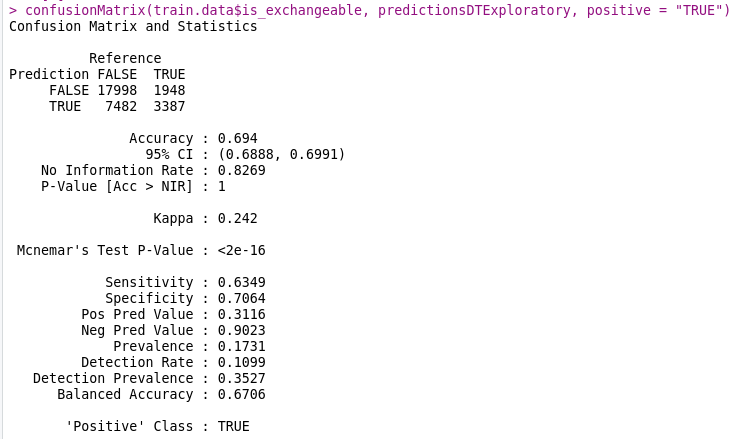
\includegraphics{images/Exchange QS/Decision Tree/DTCMExplorative.PNG}

The Accuracy for when we have an exchangeability of ``TRUE'' is
\textasciitilde63.5\%(sensitivity)

The Accuracy for when we have an exchangeability of ``False'' is
\textasciitilde70.6\%(sensitivity)

The model precision of the proportion of positive predicted value is
31.16\%.

\begin{Shaded}
\begin{Highlighting}[]
\CommentTok{\# Compute roc}
\NormalTok{predictionsDTExploratoryProb }\OtherTok{\textless{}{-}} \FunctionTok{predict}\NormalTok{(model\_DT\_Exchangeable, train.data, }\AttributeTok{type =} \StringTok{"prob"}\NormalTok{)}
\NormalTok{res.roc }\OtherTok{\textless{}{-}} \FunctionTok{roc}\NormalTok{(train.data}\SpecialCharTok{$}\NormalTok{is\_exchangeable }\SpecialCharTok{\textasciitilde{}}\NormalTok{ predictionsDTExploratoryProb[,}\DecValTok{2}\NormalTok{])}
\FunctionTok{plot.roc}\NormalTok{(res.roc, }\AttributeTok{print.auc =} \ConstantTok{TRUE}\NormalTok{)}
\FunctionTok{as.numeric}\NormalTok{(res.roc}\SpecialCharTok{$}\NormalTok{auc)}
\CommentTok{\# [1] 0.6571428}

\CommentTok{\# Get the probability threshold for specificity = 0.5}
\NormalTok{rocModelDT.data }\OtherTok{\textless{}{-}} \FunctionTok{data\_frame}\NormalTok{(}
  \AttributeTok{thresholds =}\NormalTok{ res.roc}\SpecialCharTok{$}\NormalTok{thresholds,}
  \AttributeTok{sensitivity =}\NormalTok{ res.roc}\SpecialCharTok{$}\NormalTok{sensitivities,}
  \AttributeTok{specificity =}\NormalTok{ res.roc}\SpecialCharTok{$}\NormalTok{specificities}
\NormalTok{)}
\NormalTok{rocModelDT.data }\SpecialCharTok{\%\textgreater{}\%} \FunctionTok{filter}\NormalTok{(specificity }\SpecialCharTok{\textgreater{}=} \FloatTok{0.5}\NormalTok{)}
\FunctionTok{plot.roc}\NormalTok{(res.roc, }\AttributeTok{print.auc =} \ConstantTok{TRUE}\NormalTok{, }\AttributeTok{print.thres =} \StringTok{"best"}\NormalTok{)}
\end{Highlighting}
\end{Shaded}

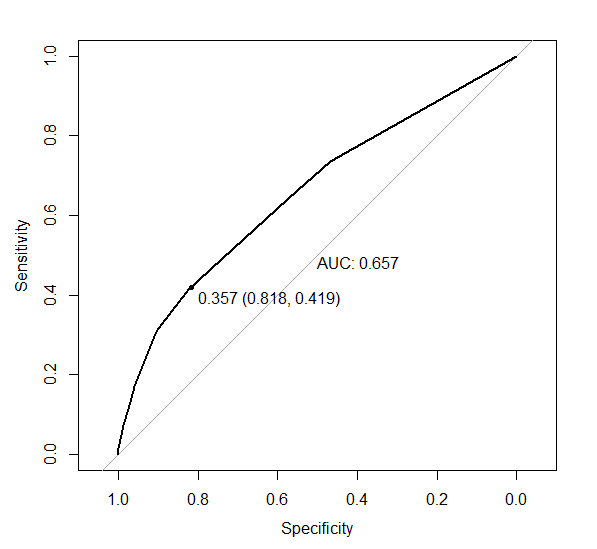
\includegraphics{images/Exchange QS/Decision Tree/DTExploratoryplot.Bestroc.png}

The AUC is above 0.5 which tells us that this is good exploratory model.
The best threshold with the highest sum sensitivity and specificity is
0.357 and we get a specificity of 0.818 and a sensitivity of 0.419.

\hypertarget{predicting-exchangeability-using-a-decision-tree}{%
\paragraph{Predicting Exchangeability using a Decision
Tree}\label{predicting-exchangeability-using-a-decision-tree}}

To analyze the predictive power of our model we used the testing
dataset.

\begin{Shaded}
\begin{Highlighting}[]
\CommentTok{\# Predictive Model}
\NormalTok{predictionsDT }\OtherTok{\textless{}{-}} \FunctionTok{predict}\NormalTok{(model\_DT\_Exchangeable, test.data)}

\CommentTok{\# Check accuracy, error, and confusion matrix}
\NormalTok{accuracy }\OtherTok{\textless{}{-}} \FunctionTok{mean}\NormalTok{(test.data}\SpecialCharTok{$}\NormalTok{is\_exchangeable }\SpecialCharTok{==}\NormalTok{ predictionsDT)}
\NormalTok{accuracy}
\CommentTok{\# [1] 0.6871661}
\NormalTok{error }\OtherTok{\textless{}{-}} \FunctionTok{mean}\NormalTok{(test.data}\SpecialCharTok{$}\NormalTok{is\_exchangeable }\SpecialCharTok{!=}\NormalTok{ predictionsDT)}
\NormalTok{error}
\CommentTok{\# [1] 0.3128339}
\FunctionTok{confusionMatrix}\NormalTok{(test.data}\SpecialCharTok{$}\NormalTok{is\_exchangeable, predictionsDT)}
\end{Highlighting}
\end{Shaded}

The accuracy above tells us that the Decision Tree correctly predicted
\textasciitilde69\% of the individuals who agreed to exchanging their
vehicles. This is better than random guessing. The misclassification
error rate is \textasciitilde31\%.

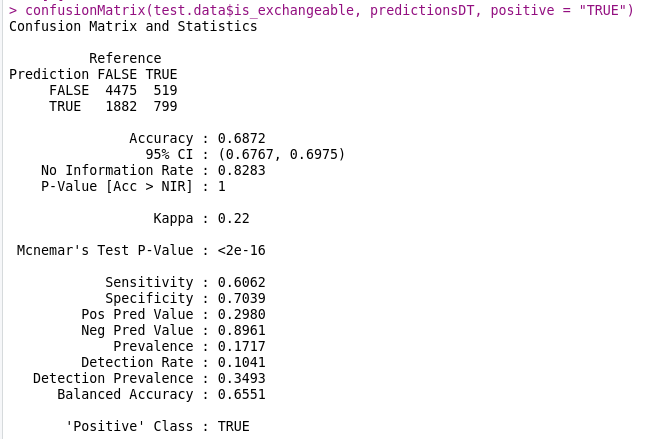
\includegraphics{images/Exchange QS/Decision Tree/DTCMPredictive.PNG}

Sensitivity is \textasciitilde60.6\%, that is the proportion of
individuals who were correctly identified to being willing to take part
in an exchange for their vehicle.

The specificity of the model is around 70.4\% which is the proportion of
individuals who were correctly identified to not being willing to take
part in an exchange for their vehicle.

The model precision or proportion of positive predicted value is
\textasciitilde{} 29.8\%

\begin{Shaded}
\begin{Highlighting}[]
\CommentTok{\#Compute roc}
\NormalTok{predictionsDTProb }\OtherTok{\textless{}{-}} \FunctionTok{predict}\NormalTok{(model\_DT\_Exchangeable, test.data, }\AttributeTok{type =} \StringTok{"prob"}\NormalTok{)}
\NormalTok{res.roc }\OtherTok{\textless{}{-}} \FunctionTok{roc}\NormalTok{(test.data}\SpecialCharTok{$}\NormalTok{is\_exchangeable }\SpecialCharTok{\textasciitilde{}}\NormalTok{ predictionsDTProb[,}\DecValTok{2}\NormalTok{])}
\FunctionTok{plot.roc}\NormalTok{(res.roc, }\AttributeTok{print.auc =} \ConstantTok{TRUE}\NormalTok{)}
\FunctionTok{as.numeric}\NormalTok{(res.roc}\SpecialCharTok{$}\NormalTok{auc)}
\CommentTok{\# [1] 0.6525616}

\CommentTok{\# Get the probability threshold for specificity = 0.5}
\NormalTok{rocModelDT.data }\OtherTok{\textless{}{-}} \FunctionTok{data\_frame}\NormalTok{(}
  \AttributeTok{thresholds =}\NormalTok{ res.roc}\SpecialCharTok{$}\NormalTok{thresholds,}
  \AttributeTok{sensitivity =}\NormalTok{ res.roc}\SpecialCharTok{$}\NormalTok{sensitivities,}
  \AttributeTok{specificity =}\NormalTok{ res.roc}\SpecialCharTok{$}\NormalTok{specificities}
\NormalTok{)}
\NormalTok{rocModelDT.data }\SpecialCharTok{\%\textgreater{}\%} \FunctionTok{filter}\NormalTok{(specificity }\SpecialCharTok{\textgreater{}=} \FloatTok{0.5}\NormalTok{)}
\FunctionTok{plot.roc}\NormalTok{(res.roc, }\AttributeTok{print.auc =} \ConstantTok{TRUE}\NormalTok{, }\AttributeTok{print.thres =} \StringTok{"best"}\NormalTok{)}
\end{Highlighting}
\end{Shaded}

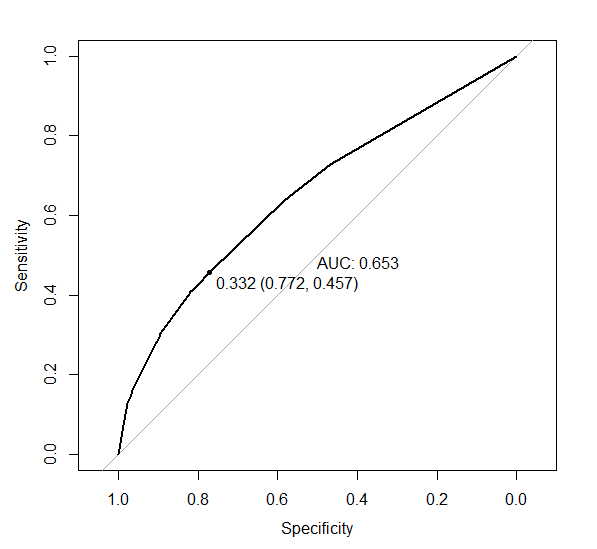
\includegraphics{images/Exchange QS/Decision Tree/DTPredictiveBestRoc.png}

In this graph the AUC is 0.653, which i relatively good. Remember that a
classifier that performs no better than chance is expected to have an
AUC of 0.5 when evaluated on an independent test set not used to train
the model. Meaning, that this model does in fact predict exchangeability
with some success. The best threshold with the highest sum sensitivity
and specificity is 0.332 and we get a specificity of 0.772 and a
sensitivity of 0.457. Ultimately, we learn that the Decision Tree
Classification produces a good predictive model for exchangeability of a
vehicle.

\hypertarget{exploring-exchangeability-using-logistic-classification}{%
\paragraph{Exploring Exchangeability using Logistic
Classification}\label{exploring-exchangeability-using-logistic-classification}}

We attempted to create a more accurate exploratory model for
exchangeability by using Logistic Classification. The model will be
running the train function with 10-fold cross-validation and a
tune-length of 10(number of cp values to evaluate). These settings
should produce an optimal model.

\begin{Shaded}
\begin{Highlighting}[]
\DocumentationTok{\#\# Using Logistic Classification to create an exploratory model for exchangeability}
\FunctionTok{set.seed}\NormalTok{(}\DecValTok{123}\NormalTok{)}
\NormalTok{model\_LR\_Exchangeable }\OtherTok{\textless{}{-}}  \FunctionTok{train}\NormalTok{( is\_exchangeable }\SpecialCharTok{\textasciitilde{}}\NormalTok{ . }\SpecialCharTok{{-}}\NormalTok{model\_name, }\AttributeTok{data =}\NormalTok{ train.data, }\AttributeTok{method =} \StringTok{"glm"}\NormalTok{, }\AttributeTok{family =} \StringTok{"binomial"}\NormalTok{,}
                                 \AttributeTok{trControl =} \FunctionTok{trainControl}\NormalTok{(}\StringTok{"cv"}\NormalTok{, }\AttributeTok{number =}\DecValTok{10}\NormalTok{),}
                                 \AttributeTok{preProcess =} \FunctionTok{c}\NormalTok{(}\StringTok{"center"}\NormalTok{, }\StringTok{"scale"}\NormalTok{),}
                                 \AttributeTok{tuneLength =} \DecValTok{10}
\NormalTok{)}

\CommentTok{\# Exploratory}
\NormalTok{predictionsLRExploratory }\OtherTok{\textless{}{-}} \FunctionTok{predict}\NormalTok{(model\_LR\_Exchangeable, train.data)}

\CommentTok{\# Check accuracy, error, and confusion matrix}
\NormalTok{accuracy }\OtherTok{\textless{}{-}} \FunctionTok{mean}\NormalTok{(train.data}\SpecialCharTok{$}\NormalTok{is\_exchangeable }\SpecialCharTok{==}\NormalTok{ predictionsLRExploratory)}
\NormalTok{accuracy}
\CommentTok{\# [1] 0.6624371       }
\NormalTok{error }\OtherTok{\textless{}{-}} \FunctionTok{mean}\NormalTok{(train.data}\SpecialCharTok{$}\NormalTok{is\_exchangeable }\SpecialCharTok{!=}\NormalTok{ predictionsLRExploratory)}
\NormalTok{error}
\CommentTok{\# [1] 0.3375629       }
\FunctionTok{confusionMatrix}\NormalTok{(train.data}\SpecialCharTok{$}\NormalTok{is\_exchangeable, predictionsLRExploratory)}
\end{Highlighting}
\end{Shaded}

The accuracy above tells us that the Logistic Classification correctly
predicted \textasciitilde66\% of the individuals who agreed to
exchanging their vehicles. This is better than random guessing. The
misclassification error rate is \textasciitilde33.76\%.

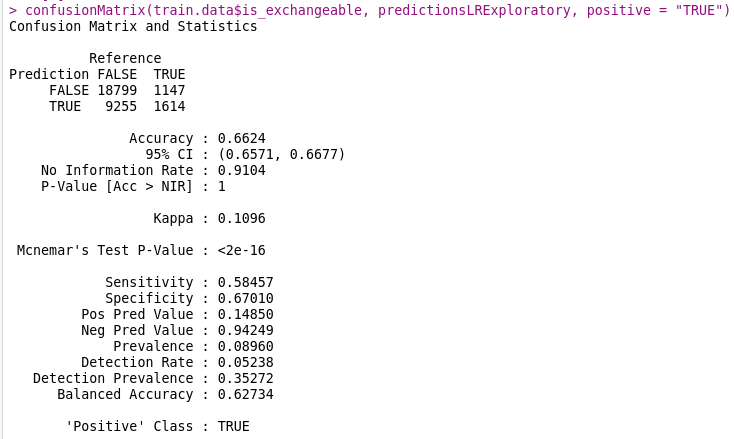
\includegraphics{images/Exchange QS/Logistic/LRCMExploratory.png}

Sensitivity is \textasciitilde58.46\%, that is the proportion of
individuals who were correctly identified to being willing to take part
in an exchange for their vehicle.

The specificity of the model is around 67\% which is the proportion of
individuals who were correctly identified to not being willing to take
part in an exchange for their vehicle.

The model precision or proportion of positive predicted value is
\textasciitilde{} 14.85\%

\begin{Shaded}
\begin{Highlighting}[]
\CommentTok{\# Compute roc}
\NormalTok{predictionsLRExploratoryProb }\OtherTok{\textless{}{-}} \FunctionTok{predict}\NormalTok{(model\_LR\_Exchangeable, train.data, }\AttributeTok{type =} \StringTok{"prob"}\NormalTok{)}
\NormalTok{res.roc }\OtherTok{\textless{}{-}} \FunctionTok{roc}\NormalTok{(train.data}\SpecialCharTok{$}\NormalTok{is\_exchangeable }\SpecialCharTok{\textasciitilde{}}\NormalTok{ predictionsLRExploratoryProb[,}\DecValTok{2}\NormalTok{])}
\FunctionTok{plot.roc}\NormalTok{(res.roc, }\AttributeTok{print.auc =} \ConstantTok{TRUE}\NormalTok{)}
\FunctionTok{as.numeric}\NormalTok{(res.roc}\SpecialCharTok{$}\NormalTok{auc)}
\CommentTok{\# [1] 0.6505955}

\CommentTok{\# Get the probability threshold for specificity = 0.5}
\NormalTok{rocModelLRExploratory.data }\OtherTok{\textless{}{-}} \FunctionTok{data\_frame}\NormalTok{(}
  \AttributeTok{thresholds =}\NormalTok{ res.roc}\SpecialCharTok{$}\NormalTok{thresholds,}
  \AttributeTok{sensitivity =}\NormalTok{ res.roc}\SpecialCharTok{$}\NormalTok{sensitivities,}
  \AttributeTok{specificity =}\NormalTok{ res.roc}\SpecialCharTok{$}\NormalTok{specificities}
\NormalTok{)}
\NormalTok{rocModelLRExploratory.data }\SpecialCharTok{\%\textgreater{}\%} \FunctionTok{filter}\NormalTok{(specificity }\SpecialCharTok{\textgreater{}=} \FloatTok{0.5}\NormalTok{)}
\FunctionTok{plot.roc}\NormalTok{(res.roc, }\AttributeTok{print.auc =} \ConstantTok{TRUE}\NormalTok{, }\AttributeTok{print.thres =} \StringTok{"best"}\NormalTok{)}
\end{Highlighting}
\end{Shaded}

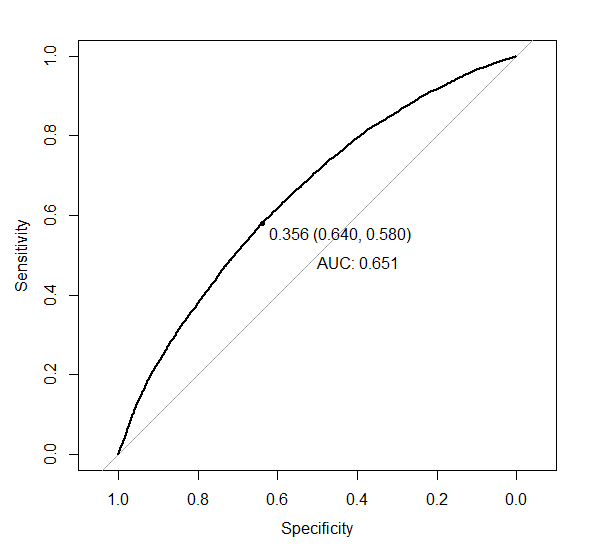
\includegraphics{images/Exchange QS/Logistic/LRExplorataryBestRoc.png}

In this graph the AUC is 0.651, which i relatively good and quite like
the AUC from the Decision Tree model. Since the classifier is better
that 0.5, we can comfortably say that this is a good exploratory model.
The best threshold with the highest sum sensitivity and specificity is
0.356 and we get a specificity of 0.640 and a sensitivity of 0.580. The
Logistic Regression Model also produces a good exploratory model.

\hypertarget{predicting-exchangeability-using-logistic-regression}{%
\paragraph{Predicting Exchangeability using Logistic
Regression}\label{predicting-exchangeability-using-logistic-regression}}

\begin{Shaded}
\begin{Highlighting}[]
\DocumentationTok{\#\# Using Logistic Regression to predict exchangeability}
\FunctionTok{set.seed}\NormalTok{(}\DecValTok{123}\NormalTok{)}
\NormalTok{model\_LR\_Exchangeable }\OtherTok{\textless{}{-}}  \FunctionTok{train}\NormalTok{( is\_exchangeable }\SpecialCharTok{\textasciitilde{}}\NormalTok{ ., }\AttributeTok{data =}\NormalTok{ train.data, }\AttributeTok{method =} \StringTok{"glm"}\NormalTok{, }\AttributeTok{family =} \StringTok{"binomial"}\NormalTok{,}
                                 \AttributeTok{trControl =} \FunctionTok{trainControl}\NormalTok{(}\StringTok{"cv"}\NormalTok{, }\AttributeTok{number =}\DecValTok{10}\NormalTok{),}
                                 \AttributeTok{preProcess =} \FunctionTok{c}\NormalTok{(}\StringTok{"center"}\NormalTok{, }\StringTok{"scale"}\NormalTok{),}
                                 \AttributeTok{tuneLength =} \DecValTok{10}
\NormalTok{)}

\NormalTok{predictionsLR }\OtherTok{\textless{}{-}} \FunctionTok{predict}\NormalTok{(model\_LR\_Exchangeable, test.data)}
\CommentTok{\# Check accuracy, error, and confusion matrix}
\NormalTok{accuracy }\OtherTok{\textless{}{-}} \FunctionTok{mean}\NormalTok{(test.data}\SpecialCharTok{$}\NormalTok{is\_exchangeable }\SpecialCharTok{==}\NormalTok{ predictionsLR)}
\NormalTok{accuracy}
\CommentTok{\# [1] 0.6650163}
\NormalTok{error }\OtherTok{\textless{}{-}} \FunctionTok{mean}\NormalTok{(test.data}\SpecialCharTok{$}\NormalTok{is\_exchangeable }\SpecialCharTok{!=}\NormalTok{ predictionsLR)}
\NormalTok{error}
\CommentTok{\# [1] 0.3349837}
\FunctionTok{confusionMatrix}\NormalTok{(test.data}\SpecialCharTok{$}\NormalTok{is\_exchangeable, predictionsLR)}
\end{Highlighting}
\end{Shaded}

The accuracy above tells us that the Logistic Classification correctly
predicted \textasciitilde66.5\% of the individuals who agreed to
exchanging their vehicles. This is a good accuracy for a predictive
model. The misclassification error rate is \textasciitilde33.5\%.

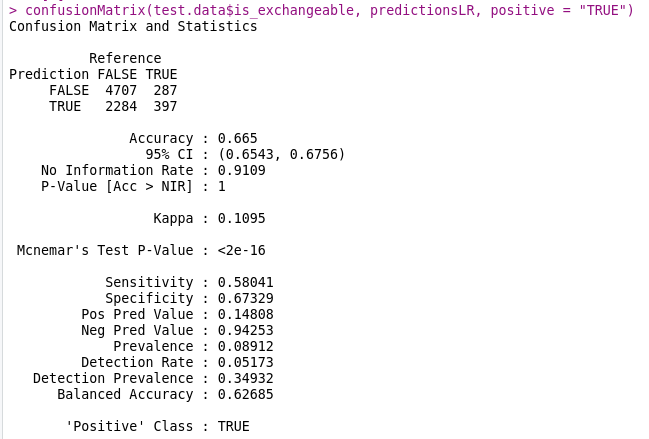
\includegraphics{images/Exchange QS/Logistic/LRCMPredictive.png}

Sensitivity is \textasciitilde58\% , that is the proportion of
individuals who were correctly identified to being willing to take part
in an exchange for their vehicle.

The specificity of the model is around 67.3\% which is the proportion of
individuals who were correctly identified to not being willing to take
part in an exchange for their vehicle.

The model precision or proportion of positive predicted value is
\textasciitilde14.8\%

\begin{Shaded}
\begin{Highlighting}[]
\CommentTok{\#Compute roc}
\NormalTok{predictionsLRProb }\OtherTok{\textless{}{-}} \FunctionTok{predict}\NormalTok{(model\_LR\_Exchangeable, test.data, }\AttributeTok{type =} \StringTok{"prob"}\NormalTok{)}
\NormalTok{res.rocLR }\OtherTok{\textless{}{-}} \FunctionTok{roc}\NormalTok{(test.data}\SpecialCharTok{$}\NormalTok{is\_exchangeable }\SpecialCharTok{\textasciitilde{}}\NormalTok{ predictionsLRProb[,}\DecValTok{2}\NormalTok{])}
\FunctionTok{plot.roc}\NormalTok{(res.rocLR, }\AttributeTok{print.auc =} \ConstantTok{TRUE}\NormalTok{)}
\FunctionTok{as.numeric}\NormalTok{(res.rocLR}\SpecialCharTok{$}\NormalTok{auc)}
\CommentTok{\# [1] 0.6480223}


\CommentTok{\# Get the probability threshold for specificity = 0.5}
\NormalTok{rocModelLR.data }\OtherTok{\textless{}{-}} \FunctionTok{data\_frame}\NormalTok{(}
  \AttributeTok{thresholds =}\NormalTok{ res.rocLR}\SpecialCharTok{$}\NormalTok{thresholds,}
  \AttributeTok{sensitivity =}\NormalTok{ res.rocLR}\SpecialCharTok{$}\NormalTok{sensitivities,}
  \AttributeTok{specificity =}\NormalTok{ res.rocLR}\SpecialCharTok{$}\NormalTok{specificities}
\NormalTok{)}
\NormalTok{rocModelLR.data }\SpecialCharTok{\%\textgreater{}\%} \FunctionTok{filter}\NormalTok{(specificity }\SpecialCharTok{\textgreater{}=} \FloatTok{0.5}\NormalTok{)}
\FunctionTok{plot.roc}\NormalTok{(res.rocLR, }\AttributeTok{print.auc =} \ConstantTok{TRUE}\NormalTok{, }\AttributeTok{print.thres =} \StringTok{"best"}\NormalTok{)}
\end{Highlighting}
\end{Shaded}

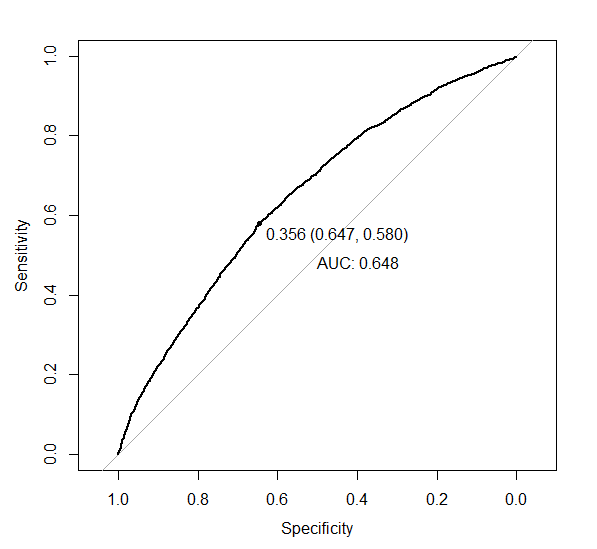
\includegraphics{images/Exchange QS/Logistic/LRPredictiveBestRoc.png}

In this graph the AUC is 0.648 is a good AUC from a model. This model
does predict exchangeability with success. The best threshold with the
highest sum sensitivity and specificity is 0.356 and we get a
specificity of 0.647 and a sensitivity of 0.580. The Logistic Regression
Model also produces a good predictive model.

\begin{longtable}[]{@{}lllllll@{}}
\toprule
\begin{minipage}[b]{(\columnwidth - 6\tabcolsep) * \real{0.35}}\raggedright
Models\strut
\end{minipage} &
\begin{minipage}[b]{(\columnwidth - 6\tabcolsep) * \real{0.08}}\raggedright
Accuracy\strut
\end{minipage} &
\begin{minipage}[b]{(\columnwidth - 6\tabcolsep) * \real{0.08}}\raggedright
Error\strut
\end{minipage} &
\begin{minipage}[b]{(\columnwidth - 6\tabcolsep) * \real{0.10}}\raggedright
Sensitivity\strut
\end{minipage} &
\begin{minipage}[b]{(\columnwidth - 6\tabcolsep) * \real{0.10}}\raggedright
Specificity\strut
\end{minipage} &
\begin{minipage}[b]{(\columnwidth - 6\tabcolsep) * \real{0.20}}\raggedright
Positive Prediction Value\strut
\end{minipage} &
\begin{minipage}[b]{(\columnwidth - 6\tabcolsep) * \real{0.08}}\raggedright
AUC\strut
\end{minipage}\tabularnewline
\midrule
\endhead
\begin{minipage}[t]{(\columnwidth - 6\tabcolsep) * \real{0.35}}\raggedright
Decision Tree Classification: Exploratory Model\strut
\end{minipage} &
\begin{minipage}[t]{(\columnwidth - 6\tabcolsep) * \real{0.08}}\raggedright
0.6939802\strut
\end{minipage} &
\begin{minipage}[t]{(\columnwidth - 6\tabcolsep) * \real{0.08}}\raggedright
0.3060198\strut
\end{minipage} &
\begin{minipage}[t]{(\columnwidth - 6\tabcolsep) * \real{0.10}}\raggedright
0.6349\strut
\end{minipage} &
\begin{minipage}[t]{(\columnwidth - 6\tabcolsep) * \real{0.10}}\raggedright
0.7064\strut
\end{minipage} &
\begin{minipage}[t]{(\columnwidth - 6\tabcolsep) * \real{0.20}}\raggedright
0.3116\strut
\end{minipage} &
\begin{minipage}[t]{(\columnwidth - 6\tabcolsep) * \real{0.08}}\raggedright
0.6571428\strut
\end{minipage}\tabularnewline
\begin{minipage}[t]{(\columnwidth - 6\tabcolsep) * \real{0.35}}\raggedright
Logistic Classification: Exploratory Model\strut
\end{minipage} &
\begin{minipage}[t]{(\columnwidth - 6\tabcolsep) * \real{0.08}}\raggedright
0.6624371\strut
\end{minipage} &
\begin{minipage}[t]{(\columnwidth - 6\tabcolsep) * \real{0.08}}\raggedright
0.3375629\strut
\end{minipage} &
\begin{minipage}[t]{(\columnwidth - 6\tabcolsep) * \real{0.10}}\raggedright
0.58457\strut
\end{minipage} &
\begin{minipage}[t]{(\columnwidth - 6\tabcolsep) * \real{0.10}}\raggedright
0.67010\strut
\end{minipage} &
\begin{minipage}[t]{(\columnwidth - 6\tabcolsep) * \real{0.20}}\raggedright
0.14850\strut
\end{minipage} &
\begin{minipage}[t]{(\columnwidth - 6\tabcolsep) * \real{0.08}}\raggedright
0.6505955\strut
\end{minipage}\tabularnewline
\begin{minipage}[t]{(\columnwidth - 6\tabcolsep) * \real{0.35}}\raggedright
Decision Tree Classification: Prediction Model\strut
\end{minipage} &
\begin{minipage}[t]{(\columnwidth - 6\tabcolsep) * \real{0.08}}\raggedright
0.6871661\strut
\end{minipage} &
\begin{minipage}[t]{(\columnwidth - 6\tabcolsep) * \real{0.08}}\raggedright
0.3128339\strut
\end{minipage} &
\begin{minipage}[t]{(\columnwidth - 6\tabcolsep) * \real{0.10}}\raggedright
0.6062\strut
\end{minipage} &
\begin{minipage}[t]{(\columnwidth - 6\tabcolsep) * \real{0.10}}\raggedright
0.7039\strut
\end{minipage} &
\begin{minipage}[t]{(\columnwidth - 6\tabcolsep) * \real{0.20}}\raggedright
0.2980\strut
\end{minipage} &
\begin{minipage}[t]{(\columnwidth - 6\tabcolsep) * \real{0.08}}\raggedright
0.6525616\strut
\end{minipage}\tabularnewline
\begin{minipage}[t]{(\columnwidth - 6\tabcolsep) * \real{0.35}}\raggedright
Logistic Classification: Prediction Model\strut
\end{minipage} &
\begin{minipage}[t]{(\columnwidth - 6\tabcolsep) * \real{0.08}}\raggedright
0.6650163\strut
\end{minipage} &
\begin{minipage}[t]{(\columnwidth - 6\tabcolsep) * \real{0.08}}\raggedright
0.3349837\strut
\end{minipage} &
\begin{minipage}[t]{(\columnwidth - 6\tabcolsep) * \real{0.10}}\raggedright
0.58041\strut
\end{minipage} &
\begin{minipage}[t]{(\columnwidth - 6\tabcolsep) * \real{0.10}}\raggedright
0.67329\strut
\end{minipage} &
\begin{minipage}[t]{(\columnwidth - 6\tabcolsep) * \real{0.20}}\raggedright
0.14808\strut
\end{minipage} &
\begin{minipage}[t]{(\columnwidth - 6\tabcolsep) * \real{0.08}}\raggedright
0.6480223\strut
\end{minipage}\tabularnewline
\bottomrule
\end{longtable}

\hypertarget{model-results-and-comparisons}{%
\subsection{Model Results and
Comparisons}\label{model-results-and-comparisons}}

To create the most accurate and significant predictive model we created
6 different models which had a wide range of accuracy.

\hypertarget{linear-regression-model}{%
\subsubsection{Linear Regression Model}\label{linear-regression-model}}

Firstly, we created a Multiple Linear Regression Model which utilized
the attributes in our dataset (except model\_names) and optimized the
model. The code for this looks as follows:

\begin{Shaded}
\begin{Highlighting}[]
\FunctionTok{set.seed}\NormalTok{(}\DecValTok{123}\NormalTok{)}
\NormalTok{LM }\OtherTok{\textless{}{-}} \FunctionTok{lm}\NormalTok{(price\_usd }\SpecialCharTok{\textasciitilde{}}\NormalTok{ odometer\_value}
         \SpecialCharTok{+}\NormalTok{ year\_produced}
         \SpecialCharTok{+}\NormalTok{ number\_of\_photos}
         \SpecialCharTok{+}\NormalTok{ duration\_listed}
         \SpecialCharTok{+}\NormalTok{ up\_counter, }\AttributeTok{data =}\NormalTok{ train.data)}
\NormalTok{step.LM }\OtherTok{\textless{}{-}}\NormalTok{ LM }\SpecialCharTok{\%\textgreater{}\%} \FunctionTok{stepAIC}\NormalTok{(}\AttributeTok{trace =} \ConstantTok{FALSE}\NormalTok{)}
\end{Highlighting}
\end{Shaded}

\begin{Shaded}
\begin{Highlighting}[]
\FunctionTok{vif}\NormalTok{(step.LM)}
\end{Highlighting}
\end{Shaded}

\begin{verbatim}
##   odometer_value    year_produced number_of_photos  duration_listed 
##         1.311552         1.375432         1.088560         1.985559 
##       up_counter 
##         1.995992
\end{verbatim}

The VIF tells us that there is not significant multi-collinearity
between any of the continuous attributes.

Now that the model is created and optimized it is vital to check the
accuracy of the model. To do this we will employ our test.data to test
how accurately the Linear Regression model can predict the price of a
vehicle.

\begin{Shaded}
\begin{Highlighting}[]
\FunctionTok{summary}\NormalTok{(step.LM)}
\end{Highlighting}
\end{Shaded}

\begin{verbatim}
## 
## Call:
## lm(formula = price_usd ~ odometer_value + year_produced + number_of_photos + 
##     duration_listed + up_counter, data = train.data)
## 
## Residuals:
##    Min     1Q Median     3Q    Max 
## -15620  -2427   -834   1352  46600 
## 
## Coefficients:
##                    Estimate Std. Error  t value Pr(>|t|)    
## (Intercept)      -9.916e+05  7.305e+03 -135.756  < 2e-16 ***
## odometer_value   -4.419e-03  2.113e-04  -20.919  < 2e-16 ***
## year_produced     4.981e+02  3.639e+00  136.895  < 2e-16 ***
## number_of_photos  1.482e+02  4.251e+00   34.854  < 2e-16 ***
## duration_listed   2.242e+00  3.143e-01    7.134 9.98e-13 ***
## up_counter        2.253e+00  8.082e-01    2.787  0.00532 ** 
## ---
## Signif. codes:  0 '***' 0.001 '**' 0.01 '*' 0.05 '.' 0.1 ' ' 1
## 
## Residual standard error: 4385 on 30809 degrees of freedom
## Multiple R-squared:  0.5304, Adjusted R-squared:  0.5303 
## F-statistic:  6959 on 5 and 30809 DF,  p-value: < 2.2e-16
\end{verbatim}

\begin{Shaded}
\begin{Highlighting}[]
\FunctionTok{coef}\NormalTok{(step.LM)}
\end{Highlighting}
\end{Shaded}

\begin{verbatim}
##      (Intercept)   odometer_value    year_produced number_of_photos 
##    -9.916423e+05    -4.419525e-03     4.981272e+02     1.481601e+02 
##  duration_listed       up_counter 
##     2.241819e+00     2.252599e+00
\end{verbatim}

\begin{Shaded}
\begin{Highlighting}[]
\FunctionTok{confint}\NormalTok{(step.LM)}
\end{Highlighting}
\end{Shaded}

\begin{verbatim}
##                          2.5 %        97.5 %
## (Intercept)      -1.005960e+06 -9.773249e+05
## odometer_value   -4.833614e-03 -4.005436e-03
## year_produced     4.909951e+02  5.052594e+02
## number_of_photos  1.398282e+02  1.564919e+02
## duration_listed   1.625863e+00  2.857775e+00
## up_counter        6.685618e-01  3.836636e+00
\end{verbatim}

The information above is crucial for calculating values and having a
general idea for the stability of our coefficients.

\begin{Shaded}
\begin{Highlighting}[]
\NormalTok{LMPrediction }\OtherTok{\textless{}{-}} \FunctionTok{predict}\NormalTok{(step.LM, test.data)}

\CommentTok{\# Prediction error, rmse}
\FunctionTok{RMSE}\NormalTok{(LMPrediction,test.data}\SpecialCharTok{$}\NormalTok{price\_usd)}
\end{Highlighting}
\end{Shaded}

\begin{verbatim}
## [1] 4573.511
\end{verbatim}

\begin{Shaded}
\begin{Highlighting}[]
\CommentTok{\# Compute R{-}square}
\FunctionTok{R2}\NormalTok{(LMPrediction,test.data}\SpecialCharTok{$}\NormalTok{price\_usd)}
\end{Highlighting}
\end{Shaded}

\begin{verbatim}
## [1] 0.5095891
\end{verbatim}

From the code above we see that our \textbf{rmse is 4470.274 which
represents an error rate of 4470.274/mean(test.data\$price\_usd) =
67.57975} which is not good. Meanwhile, the \textbf{R-Squared is
0.5190641}, meaning that the observed and predicted outcome values are
not very correlated, which is not good. These results are not surprising
and inform us that the price of a vehicle in Belarus is dependent on
more attributes than simply our continuous attributes. We shall proceed
with more robust models to achieve a better result.

note: A logarithmic transformation was done on the price and achieved an
even worse result. Given the poor quality of this model we continued
with SVR to get a more robust and accurate predictive model.

\hypertarget{svr-model}{%
\subsubsection{SVR Model}\label{svr-model}}

SVR is an extremely robust model which would be able to handle our
categorical data. These models would almost certainly achieve a better
result that the Linear Regression Model. 3 SVR models were calculated
with varying accuracies. The different methods used with SVR were
linear, polynomial, and radial.

Linear was the first SVR model to be run and the code was as follows:

\begin{Shaded}
\begin{Highlighting}[]
\CommentTok{\# Create SVR Model using Linear Method}
\FunctionTok{set.seed}\NormalTok{(}\DecValTok{123}\NormalTok{)}
\NormalTok{modelSVRLinTrain }\OtherTok{\textless{}{-}} \FunctionTok{train}\NormalTok{( price\_usd }\SpecialCharTok{\textasciitilde{}}\NormalTok{ ., }\AttributeTok{data =}\NormalTok{ train.data, }\AttributeTok{method =} \StringTok{"svmLinear"}\NormalTok{,}
                           \AttributeTok{trControl =} \FunctionTok{trainControl}\NormalTok{(}\StringTok{"cv"}\NormalTok{, }\AttributeTok{number =}\DecValTok{10}\NormalTok{),}
                           \AttributeTok{preProcess =} \FunctionTok{c}\NormalTok{(}\StringTok{"center"}\NormalTok{, }\StringTok{"scale"}\NormalTok{),}
                           \AttributeTok{tuneLength =} \DecValTok{10}
\NormalTok{)}

\FunctionTok{summary}\NormalTok{(modelSVRLinTrain)}
\CommentTok{\#Length  Class   Mode }
\CommentTok{\#1   ksvm     S4 }
\NormalTok{modelSVRLinTrain}\SpecialCharTok{$}\NormalTok{bestTune}
\CommentTok{\#C}
\CommentTok{\#1 1}
\end{Highlighting}
\end{Shaded}

We were able to find that the \textbf{bestTune was 1} which informs us
what the best tuning parameter C that maximizes our accuracy. We proceed
with using the model to predict our prices and comparing them to the
actual testing prices to gauge accuracy of the model.

\begin{Shaded}
\begin{Highlighting}[]
\CommentTok{\# Predict using SVR Model with Linear Method}
\NormalTok{modelSVRLinTrainPrediction }\OtherTok{\textless{}{-}} \FunctionTok{predict}\NormalTok{(modelSVRLinTrain, test.data)}

\CommentTok{\# Prediction error, rmse}
\FunctionTok{RMSE}\NormalTok{(modelSVRLinTrainPrediction,test.data}\SpecialCharTok{$}\NormalTok{price\_usd)}
\CommentTok{\#[1] 3257.453}

\CommentTok{\# Compute R{-}square}
\FunctionTok{R2}\NormalTok{(modelSVRLinTrainPrediction,test.data}\SpecialCharTok{$}\NormalTok{price\_usd)}
\CommentTok{\#[1] 0.777241}
\end{Highlighting}
\end{Shaded}

Observing RMSE(\textbf{3257.453}) we can see how concentrated the data
is around our model. \textbf{Calculating our error rate, we see
3257.453/mean(test.data\$price\_usd) *100 = 48.86270} is not great, but
significantly better than our Linear Regression Model. Also, a
\textbf{R-Squared of 0.7772410} is a significant increase in accuracy as
well. We know that around 77.7\% of our prices can be explained by our
model. Nevertheless, we continue to find better models:

The next model to be computed is the SVR model using the polynomial
method: This model was not able to compute in time and would be a
wonderful model to check given more time.

\begin{Shaded}
\begin{Highlighting}[]
\CommentTok{\# Create SVR Model using Polynomial Method}
\FunctionTok{set.seed}\NormalTok{(}\DecValTok{123}\NormalTok{)}
\NormalTok{modelSVRPolyTrain }\OtherTok{\textless{}{-}} \FunctionTok{train}\NormalTok{(price\_usd }\SpecialCharTok{\textasciitilde{}}\NormalTok{ ., }\AttributeTok{data =}\NormalTok{ train.data, }\AttributeTok{method =} \StringTok{"svmPoly"}\NormalTok{,}
                           \AttributeTok{trControl =} \FunctionTok{trainControl}\NormalTok{(}\StringTok{"cv"}\NormalTok{, }\AttributeTok{number =}\DecValTok{10}\NormalTok{),}
                           \AttributeTok{preProcess =} \FunctionTok{c}\NormalTok{(}\StringTok{"center"}\NormalTok{, }\StringTok{"scale"}\NormalTok{),}
                           \AttributeTok{tuneLength =} \DecValTok{10}
\NormalTok{)}

\FunctionTok{summary}\NormalTok{(modelSVRPolyTrain)}
\NormalTok{modelSVRPolyTrain}\SpecialCharTok{$}\NormalTok{bestTune}
\end{Highlighting}
\end{Shaded}

\begin{Shaded}
\begin{Highlighting}[]
\CommentTok{\# Predict using SVR Model with Linear Method}
\NormalTok{modelSVRPolyTrainPrediction }\OtherTok{\textless{}{-}} \FunctionTok{predict}\NormalTok{(modelSVRPolyTrain, test.data)}

\CommentTok{\# Prediction error, rmse}
\FunctionTok{RMSE}\NormalTok{(modelSVRPolyTrainPrediction,test.data}\SpecialCharTok{$}\NormalTok{price\_usd)}

\CommentTok{\# Compute R{-}square}
\FunctionTok{R2}\NormalTok{(modelSVRPolyTrainPrediction,test.data}\SpecialCharTok{$}\NormalTok{price\_usd)}
\end{Highlighting}
\end{Shaded}

Lastly, the radial method was used with the SVR model:

\begin{Shaded}
\begin{Highlighting}[]
\CommentTok{\# Create SVR Model using Radial Method}
\FunctionTok{set.seed}\NormalTok{(}\DecValTok{123}\NormalTok{)}
\NormalTok{modelSVRRadialTrain }\OtherTok{\textless{}{-}} \FunctionTok{train}\NormalTok{(price\_usd }\SpecialCharTok{\textasciitilde{}}\NormalTok{ ., }\AttributeTok{data =}\NormalTok{ train.data, }\AttributeTok{method =} \StringTok{"svmRadial"}\NormalTok{,}
                             \AttributeTok{trControl =} \FunctionTok{trainControl}\NormalTok{(}\StringTok{"cv"}\NormalTok{, }\AttributeTok{number =}\DecValTok{10}\NormalTok{),}
                             \AttributeTok{preProcess =} \FunctionTok{c}\NormalTok{(}\StringTok{"center"}\NormalTok{, }\StringTok{"scale"}\NormalTok{),}
                             \AttributeTok{tuneLength =} \DecValTok{10}
\NormalTok{)}

\FunctionTok{summary}\NormalTok{(modelSVRRadialTrain)}
\CommentTok{\#Length  Class   Mode}
\CommentTok{\#1   ksvm     S4                     }
\NormalTok{modelSVRRadialTrain}\SpecialCharTok{$}\NormalTok{bestTune}
\CommentTok{\#sigma   C}
\CommentTok{\#10 0.001556481 128 }
\end{Highlighting}
\end{Shaded}

\textbf{BestTune was 128} which tells us what the best tuning parameter
C that maximizes our accuracy is 128. We then used our model to predict
prices of vehicles and compared those prices to the actual testing
prices to assess the accuracy of the model.

\begin{Shaded}
\begin{Highlighting}[]
\CommentTok{\# Predict using SVR Model with Radial Method}
\NormalTok{modelSVRRadialTrainPrediction }\OtherTok{\textless{}{-}} \FunctionTok{predict}\NormalTok{(modelSVRRadialTrain, test.data)}

\CommentTok{\# Prediction error, rmse}
\FunctionTok{RMSE}\NormalTok{(modelSVRRadialTrainPrediction,test.data}\SpecialCharTok{$}\NormalTok{price\_usd)}
\CommentTok{\#[1] 4752.231}

\CommentTok{\# Compute R{-}square}
\FunctionTok{R2}\NormalTok{(modelSVRRadialTrainPrediction,test.data}\SpecialCharTok{$}\NormalTok{price\_usd)}
\CommentTok{\#[1] 0.5937837}
\end{Highlighting}
\end{Shaded}

\textbf{From the RMSE(4752.231) we calculated our error rate as
4752.231/mean(test.data\$price\_usd) *100 = 71.28478.} This is even
worse than the results we had from the Linear Regression Model. Not
surprisingly our R2 was also quite poor. \textbf{The R-Squared was
0.5937837} which again is not a good value. We know that around 59.4\%
of our prices can be explained by our model. These results convince us
that radial basis functions are not the optimal function to be used with
SVR for our model.

Given the result one can conclude that the data may have to be scaled to
optimize the results of the model. Given more time it may be beneficial
rerun the model with the scaled dataset to see if a better result could
be achieved.

Even though the SVR model did much better as a whole than the Linear
Regression Model it was vital to investigate more models to create an
even more accurate model. The Decision Tree was a perfect candidate
since it is incredibly robust and relies on very few assumptions. Its
simpler nature also makes it a model that would be preferred over other
models (such as Random Forest Regression).

\hypertarget{decision-tree-regression-model}{%
\subsubsection{Decision Tree Regression
Model}\label{decision-tree-regression-model}}

We began our Decision Tree model by running train with 10-fold
cross-validation and a tune-length of 10(number of cp values to
evaluate) as with our SVR model. These settings pruned our tree and
ensured an optimal decision tree.

\begin{Shaded}
\begin{Highlighting}[]
\FunctionTok{set.seed}\NormalTok{(}\DecValTok{123}\NormalTok{)}
\NormalTok{model\_DT\_Train }\OtherTok{\textless{}{-}} \FunctionTok{train}\NormalTok{(price\_usd }\SpecialCharTok{\textasciitilde{}}\NormalTok{ ., }\AttributeTok{data =}\NormalTok{ train.data, }\AttributeTok{method =} \StringTok{"rpart"}\NormalTok{,}
                        \AttributeTok{trControl =} \FunctionTok{trainControl}\NormalTok{(}\StringTok{"cv"}\NormalTok{,}\AttributeTok{number =} \DecValTok{10}\NormalTok{),}
                        \AttributeTok{preProcess =} \FunctionTok{c}\NormalTok{(}\StringTok{"center"}\NormalTok{,}\StringTok{"scale"}\NormalTok{),}
                        \AttributeTok{tuneLength =} \DecValTok{10}\NormalTok{)}

\FunctionTok{summary}\NormalTok{(model\_DT\_Train)}
\CommentTok{\#See summary(model\_DT\_Train)(2nd Run).txt}
\CommentTok{\#For results}
\NormalTok{model\_DT\_Train}\SpecialCharTok{$}\NormalTok{bestTune}
\CommentTok{\#          cp}
\CommentTok{\#1 0.01032955}
\FunctionTok{plot}\NormalTok{(model\_DT\_Train)}
\end{Highlighting}
\end{Shaded}

\textbf{Our value for bestTune was 0.01032955} which tells us what the
best tuning parameter C that maximizes our accuracy is 0.01032955. The
plot below shows the relationship between RMSE and the cp values. One
can easily see that the cp value was chosen to minimize the value of the
RMSE.

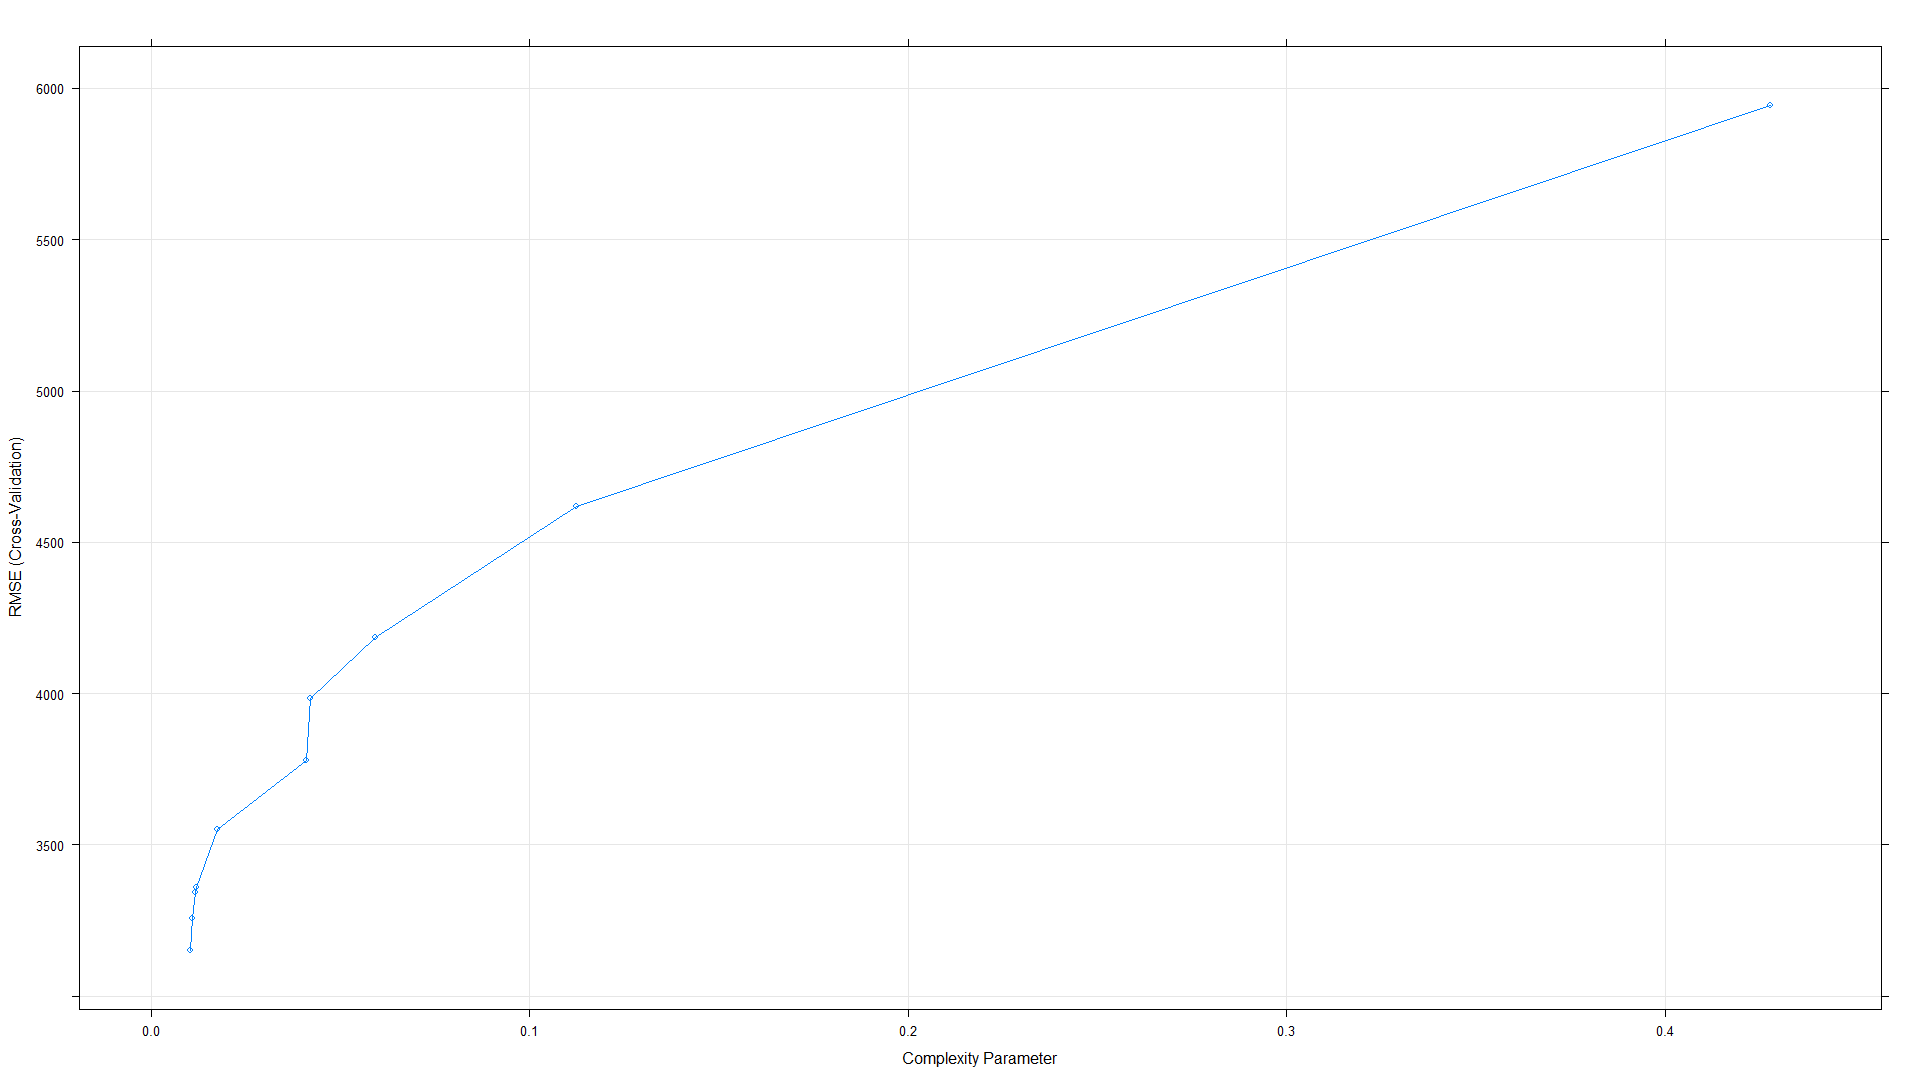
\includegraphics{images/Main Goal/Decision Tree/plot(model_DT_Train)_1920_1080.png}

Next, we will plot the final model for the decision tree as well as the
decision rules for our final model.

\begin{Shaded}
\begin{Highlighting}[]
\CommentTok{\# Plot the final tree model}
\FunctionTok{par}\NormalTok{(}\AttributeTok{xpd =} \ConstantTok{NA}\NormalTok{) }\CommentTok{\# Avoid clipping the text in some device}
\FunctionTok{plot}\NormalTok{(model\_DT\_Train}\SpecialCharTok{$}\NormalTok{finalModel)}
\FunctionTok{text}\NormalTok{(model\_DT\_Train}\SpecialCharTok{$}\NormalTok{finalModel, }\AttributeTok{digits =} \DecValTok{3}\NormalTok{)}

\CommentTok{\#Decision rules in the model}
\NormalTok{model\_DT\_Train}\SpecialCharTok{$}\NormalTok{finalModel}
\CommentTok{\# See model\_DT\_TrainfinalModel{-}1.txt}
\end{Highlighting}
\end{Shaded}

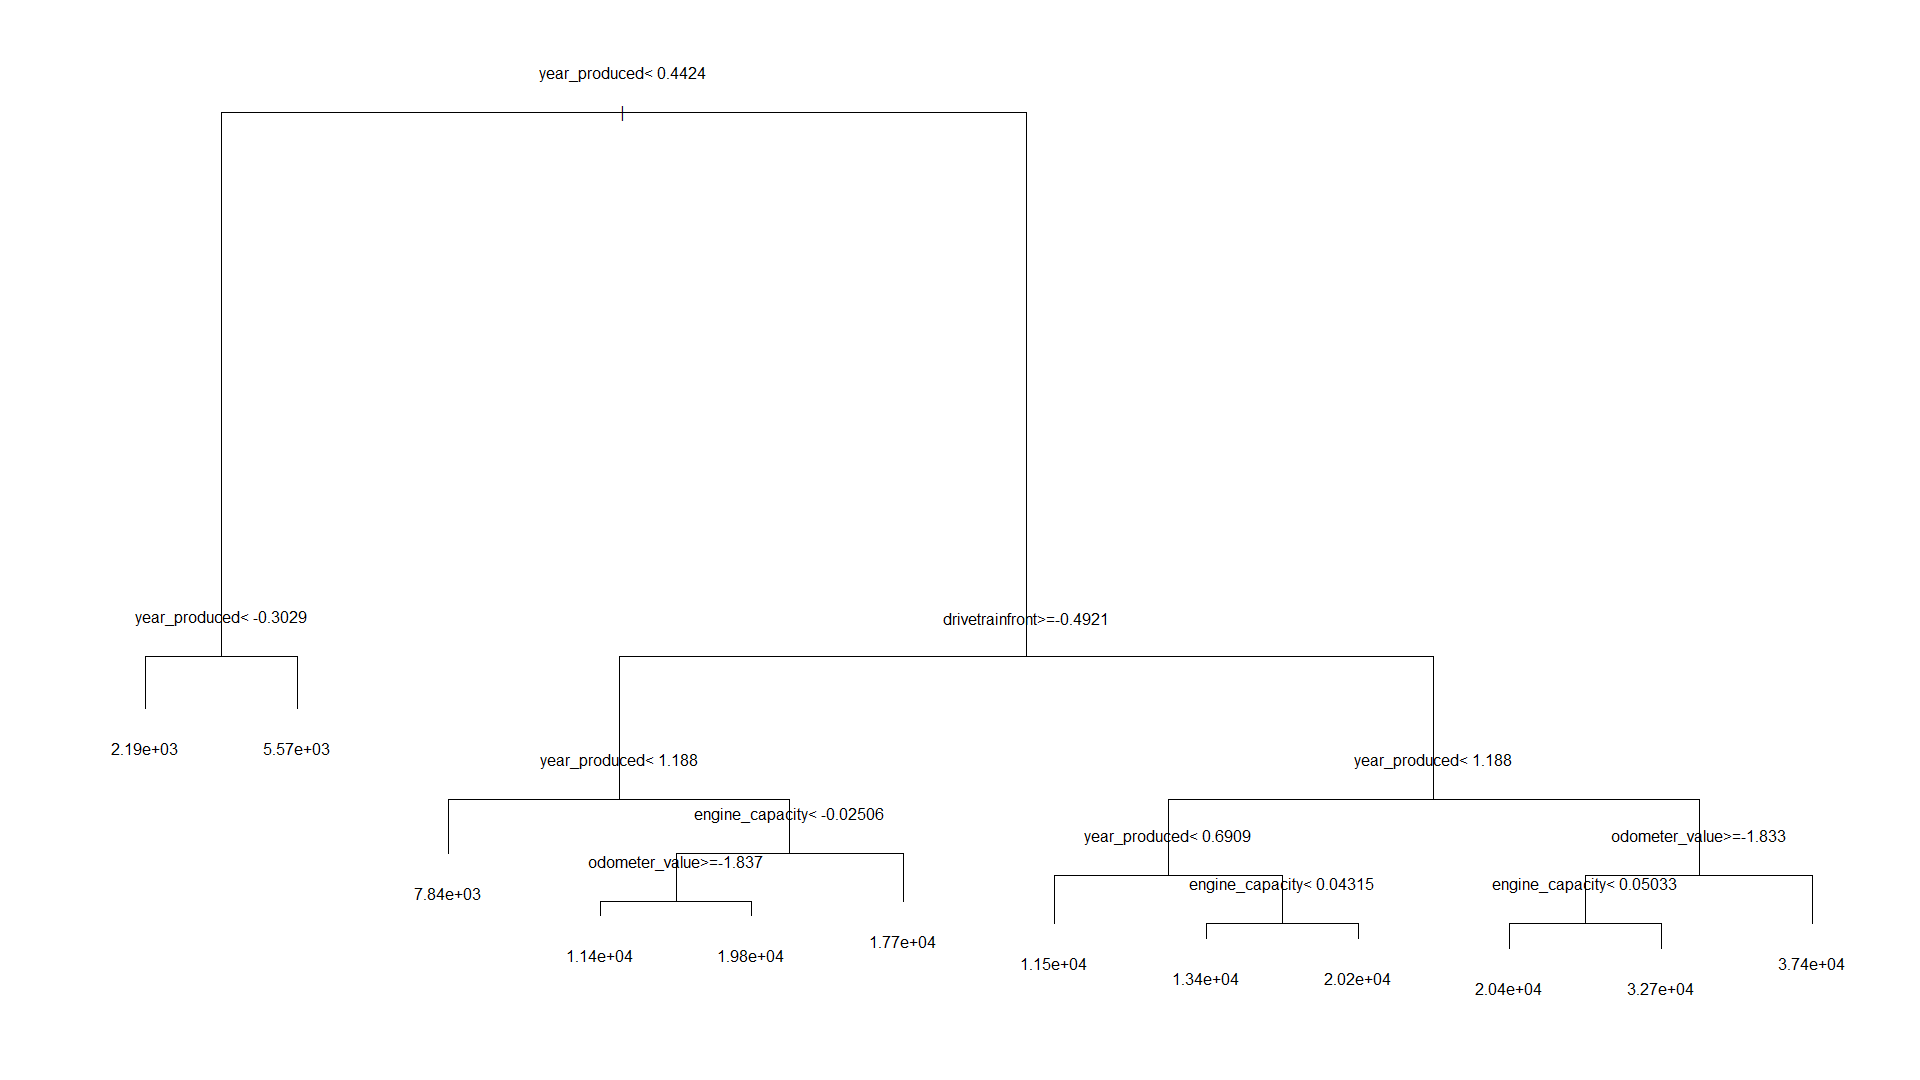
\includegraphics{images/Main Goal/Decision Tree/plot(model_DT_Train$finalModel)Text.png}

Once the Decision Tree is created and pruned, we will then use it to
predict values of our vehicle prices and analyze the accuracy of the
model.

\begin{Shaded}
\begin{Highlighting}[]
\CommentTok{\#Decision rules in the model model\_DT\_Train$finalModel}

\CommentTok{\# Make predictions on the test data }
\NormalTok{prediction\_DT\_Train }\OtherTok{\textless{}{-}}\NormalTok{ model\_DT\_Train }\SpecialCharTok{\%\textgreater{}\%} \FunctionTok{predict}\NormalTok{(test.data)}

\CommentTok{\# Prediction error, rmse}
\FunctionTok{RMSE}\NormalTok{(prediction\_DT\_Train,test.data}\SpecialCharTok{$}\NormalTok{price\_usd)}
\CommentTok{\#[1] 3245.413}

\CommentTok{\# Compute R{-}square }
\FunctionTok{R2}\NormalTok{(prediction\_DT\_Train,test.data}\SpecialCharTok{$}\NormalTok{price\_usd) }
\CommentTok{\#[1] 0.7529956}
\end{Highlighting}
\end{Shaded}

\textbf{Given the RMSE being 3245.413 we calculated our error rate as
3245.413/mean(test.data\$price\_usd) *100 = 48.68209.} This is better
than the Linear Regression Model, as well as SVR with Linear and Radial
Kernels. Not surprisingly we have a relatively good \textbf{R-Squared at
0.7529956} which is better than all but SVR with Linear Kernel and
Linear Regression. The R-Squared tells us that around 75.3\% of our
prices can be explained by our model. These results are good, but at
this point more models could not hurt. There is no guarantee that other
models would perform better, but experimentation is optimal in a search
for a better model.

Given how well the Decision Tree model operated it would make sense to
try the Random Forest Tree Model given that the Random Forest Regression
is a more complicated application of the Decision Tree since it
leverages multiple decision trees. In essence, one can expect a better
result from the Random Forest Tree (the question lies in whether the
improvement is worth the complexity in calculation)

\hypertarget{random-forest-tree-model}{%
\subsubsection{Random Forest Tree
Model}\label{random-forest-tree-model}}

The Random Forest Tree model was run with 10-fold cross-validation and a
tune-length of 10(number of cp values to evaluate for optimization) as
with SVR and the Decision tree. These settings should ensure an optimal
Random Forest Tree Model.

\begin{Shaded}
\begin{Highlighting}[]
\FunctionTok{set.seed}\NormalTok{(}\DecValTok{123}\NormalTok{)}
\NormalTok{random\_forest\_ranger }\OtherTok{\textless{}{-}} \FunctionTok{train}\NormalTok{(price\_usd }\SpecialCharTok{\textasciitilde{}}\NormalTok{ . ,}
                              \AttributeTok{data =}\NormalTok{ train.data,}
                              \AttributeTok{method =} \StringTok{"ranger"}\NormalTok{,}
                              \AttributeTok{trControl =} \FunctionTok{trainControl}\NormalTok{(}\StringTok{"cv"}\NormalTok{, }\AttributeTok{number =} \DecValTok{10}\NormalTok{),}
                              \AttributeTok{preProcess =} \FunctionTok{c}\NormalTok{(}\StringTok{"center"}\NormalTok{,}\StringTok{"scale"}\NormalTok{),}
                              \AttributeTok{tuneLength =} \DecValTok{10}
\NormalTok{)}

\FunctionTok{summary}\NormalTok{(random\_forest\_ranger)}
\CommentTok{\#                          Length Class         Mode     }
\CommentTok{\#predictions               30815  {-}none{-}        numeric  }
\CommentTok{\#num.trees                     1  {-}none{-}        numeric  }
\CommentTok{\#num.independent.variables     1  {-}none{-}        numeric  }
\CommentTok{\#mtry                          1  {-}none{-}        numeric  }
\CommentTok{\#min.node.size                 1  {-}none{-}        numeric  }
\CommentTok{\#prediction.error              1  {-}none{-}        numeric  }
\CommentTok{\#forest                        7  ranger.forest list     }
\CommentTok{\#splitrule                     1  {-}none{-}        character}
\CommentTok{\#num.random.splits             1  {-}none{-}        numeric  }
\CommentTok{\#treetype                      1  {-}none{-}        character}
\CommentTok{\#r.squared                     1  {-}none{-}        numeric  }
\CommentTok{\#call                          9  {-}none{-}        call     }
\CommentTok{\#importance.mode               1  {-}none{-}        character}
\CommentTok{\#num.samples                   1  {-}none{-}        numeric  }
\CommentTok{\#replace                       1  {-}none{-}        logical  }
\CommentTok{\#xNames                     1215  {-}none{-}        character}
\CommentTok{\#problemType                   1  {-}none{-}        character}
\CommentTok{\#tuneValue                     3  data.frame    list     }
\CommentTok{\#obsLevels                     1  {-}none{-}        logical  }
\CommentTok{\#param                         0  {-}none{-}        list }

\NormalTok{random\_forest\_ranger}\SpecialCharTok{$}\NormalTok{finalModel}
\CommentTok{\#Ranger result}
\CommentTok{\#}
\CommentTok{\#Call:}
\CommentTok{\#  ranger::ranger(dependent.variable.name = ".outcome", data = x,      mtry = min(param$mtry, ncol(x)), min.node.size = param$min.node.size,      splitrule = as.character(param$splitrule), write.forest = TRUE,      probability = classProbs, ...) }
\CommentTok{\#}
\CommentTok{\#Type:                             Regression }
\CommentTok{\#Number of trees:                  500 }
\CommentTok{\#Sample size:                      30815 }
\CommentTok{\#Number of independent variables:  1215 }
\CommentTok{\#Mtry:                             1215 }
\CommentTok{\#Target node size:                 5 }
\CommentTok{\#Variable importance mode:         none }
\CommentTok{\#Splitrule:                        extratrees }
\CommentTok{\#Number of random splits:          1 }
\CommentTok{\#OOB prediction error (MSE):       3137444 }
\CommentTok{\#R squared (OOB):                  0.9233405 }
\end{Highlighting}
\end{Shaded}

\textbf{Below is the plot for the random forest Tree. This plot shows
the values for the model accuracy vs different values of the complexity
parameter.}

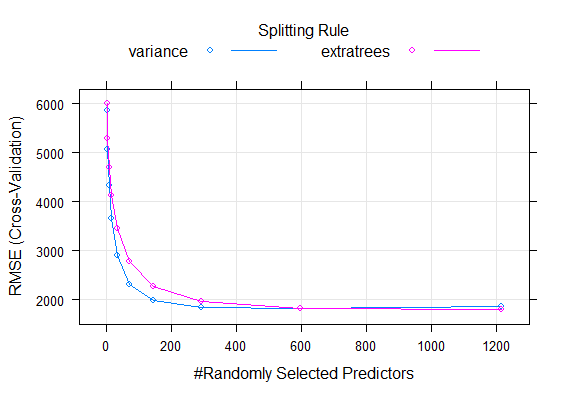
\includegraphics{images/Main Goal/Random Forest/plot(random_forest_ranger)_568_395.png}

Once the Random Forest Tree is made, we wish to gauge the accuracy of
the model. To accomplish this, we use the predict function to predict
values of our vehicle prices. Afterwards, we will compare these values
to the actual prices of the test dataset to find the accuracy of the
model.

\begin{Shaded}
\begin{Highlighting}[]
\CommentTok{\# Make predictions on the test data}
\NormalTok{rf\_predict\_ranger }\OtherTok{\textless{}{-}} \FunctionTok{predict}\NormalTok{(random\_forest\_ranger, test.data)}

\CommentTok{\# Prediction error, rmse}
\FunctionTok{RMSE}\NormalTok{(rf\_predict\_ranger,test.data}\SpecialCharTok{$}\NormalTok{price\_usd)}
\CommentTok{\#[1] 1879.884}

\CommentTok{\# Compute R{-}square}
\FunctionTok{R2}\NormalTok{(rf\_predict\_ranger,test.data}\SpecialCharTok{$}\NormalTok{price\_usd)}
\CommentTok{\#[1] 0.9184761}
\end{Highlighting}
\end{Shaded}

\textbf{The RMSE is 1879.884 we calculated our error rate as
1879.884/mean(test.data\$price\_usd) *100 = 28.19878.} This is the best
error rate so far. Not surprisingly we have a great \textbf{R-Squared at
0.9184761}. The R2 tells us that around 91.8\% of our prices can be
explained by our model. These results are the best we have so far, but
improvement may still be possible. We continue with KNN to achieve a
better result (if possible).

\hypertarget{knn-model}{%
\subsubsection{KNN Model}\label{knn-model}}

\begin{Shaded}
\begin{Highlighting}[]
\FunctionTok{set.seed}\NormalTok{(}\DecValTok{123}\NormalTok{)}
\NormalTok{model\_knn }\OtherTok{\textless{}{-}} \FunctionTok{train}\NormalTok{(}
\NormalTok{  price\_usd }\SpecialCharTok{\textasciitilde{}}\NormalTok{., }\AttributeTok{data =}\NormalTok{ train.data, }\AttributeTok{method =} \StringTok{"knn"}\NormalTok{,}
  \AttributeTok{trControl =} \FunctionTok{trainControl}\NormalTok{(}\StringTok{"cv"}\NormalTok{, }\AttributeTok{number =} \DecValTok{10}\NormalTok{),}
  \AttributeTok{preProcess =} \FunctionTok{c}\NormalTok{(}\StringTok{"center"}\NormalTok{,}\StringTok{"scale"}\NormalTok{),}
  \AttributeTok{tuneLength =} \DecValTok{20}
\NormalTok{)}

\FunctionTok{summary}\NormalTok{(model\_knn}\SpecialCharTok{$}\NormalTok{finalModel)}
\CommentTok{\#Length Class      Mode     }
\CommentTok{\#learn          2   {-}none{-}     list     }
\CommentTok{\#k              1   {-}none{-}     numeric  }
\CommentTok{\#theDots        0   {-}none{-}     list     }
\CommentTok{\#xNames      1215   {-}none{-}     character}
\CommentTok{\#problemType    1   {-}none{-}     character}
\CommentTok{\#tuneValue      1   data.frame list     }
\CommentTok{\#obsLevels      1   {-}none{-}     logical  }
\CommentTok{\#param          0   {-}none{-}     list}

\CommentTok{\# Print the best tuning parameter k that maximizes model accuracy}
\NormalTok{model\_knn}\SpecialCharTok{$}\NormalTok{bestTune}
\CommentTok{\#k}
\CommentTok{\#1 5}
\end{Highlighting}
\end{Shaded}

\textbf{A best k value was 5} tells us what the best tuning parameter K
that maximizes our accuracy is 5.

We continue our investigation of KNN by plotting the model accuracy of
KNN relative to different values of k.

\begin{Shaded}
\begin{Highlighting}[]
\CommentTok{\# Plot model accuracy vs different values of k}
\FunctionTok{plot}\NormalTok{(model\_knn)}
\end{Highlighting}
\end{Shaded}

The plot below illustrates the relationship between RMSE and cp values.
The cp value is chosen to minimize the RMSE and thus optimize the
accuracy of the graph.

{[}{]}(images/Main\%20Goal/KNN/plot(model\_knn\_seed(123)\_1920\_1080.png)

With optimization for our KNN model complete we now direct our attention
to evaluating the accuracy of the model. This is done by using the model
to predict prices from our test dataset. This ensures the model is
tested on data that is not in the training and allows us to test the
accuracy of the predictions against known values.

\begin{Shaded}
\begin{Highlighting}[]
\CommentTok{\# Make predictions on the test data}
\NormalTok{knn\_predictions }\OtherTok{\textless{}{-}}\NormalTok{ model\_knn }\SpecialCharTok{\%\textgreater{}\%} \FunctionTok{predict}\NormalTok{(test.data)}
\FunctionTok{head}\NormalTok{(knn\_predictions)}
\CommentTok{\#[1] 9560.000 8540.000 3210.000 5648.494 8575.200 7720.000}

\CommentTok{\# Compute the prediction error RMSE}
\FunctionTok{RMSE}\NormalTok{(knn\_predictions,test.data}\SpecialCharTok{$}\NormalTok{price\_usd)}
\CommentTok{\#[1] 3693.939}

\CommentTok{\# Compute R{-}square}
\FunctionTok{R2}\NormalTok{(knn\_predictions,test.data}\SpecialCharTok{$}\NormalTok{price\_usd)}
\CommentTok{\#[1] 0.680185}
\end{Highlighting}
\end{Shaded}

Given the RMSE being 3693.939 we calculated our error rate as
3693.939/mean(test.data\$price\_usd) *100 = 55.41011. \textbf{This is
better than SVR with Radial Kernel and puts it at our second lowest
performing model. The R-Squared at 0.680185} tells us that around
68.02\% of our prices can be explained by our model.

Given the result of the KNN model one can conclude that more may have to
be done to optimize the results of the model. Given more time it may be
beneficial to scale the data and rerun the model to see if a better
result could be achieved.

\hypertarget{results-obtained}{%
\subsection{Results Obtained}\label{results-obtained}}

\begin{longtable}[]{@{}lccr@{}}
\toprule
Machine-Learning Methods & RMSE & Error Rate & R-Square\tabularnewline
\midrule
\endhead
Multiple Linear Regression (Continuous) & \textbf{4470.274} &
\textbf{67.57975} & \textbf{0.5190641}\tabularnewline
SVR Linear & \textbf{3257.453} & \textbf{48.86270} &
\textbf{0.7772410}\tabularnewline
SVR Radial & \textbf{4752.231} & \textbf{71.28478} &
\textbf{0.5937837}\tabularnewline
Decision Tree Regression & \textbf{3245.413} & \textbf{48.68209} &
\textbf{0.7529956}\tabularnewline
Random Forest Tree Regression & \textbf{1879.884} & \textbf{28.19878} &
\textbf{0.9184761}\tabularnewline
KNN(K Nearest Neighbor) & \textbf{3693.939} & \textbf{55.41011} &
\textbf{0.680185}\tabularnewline
\bottomrule
\end{longtable}

\hypertarget{conclusion}{%
\subsection{Conclusion}\label{conclusion}}

We have thoroughly and exhaustively analyzed our data set with the tools
that we have learned to use through our Data Analytics course. We can
conclude that the asking price of a vehicle depends on many variables.
There are several correlations and trends that we have been able to
identify. Some vehicles do not occur often due to a limit in the data
collected and for that reason prediction made on vehicles (specifically
models) that are not common ought to be taken with the limitations of
the models in mind. More testing is needed to delve further into our
questions and optimize our models. As is the case with data science, the
process of managing data, finding new insights through analytics, and
making conclusions will continue to occur. As we find answers, we find
new questions to ask, and that is the core of data science.

\end{document}
